\section{Model Validation} \label{sec:model_validation}
In this section, the models presented in~Sections \ref{sec:power_model} and~\ref{sec:performance_model} were validated with a benchmark specific for multi-core architectures. Additionally, in order to assess the modeling overhead and accuracy, our proposal was then compared to machine learning approaches. We compared against support vector regression (SVR)~\cite{Smola2004ARegression}, decision tree \cite{Kitts2006RegressionLecture}, k-nearest neighbors \cite{Altman1992AnRegression}, multilayer perceptron \cite{Murtagh1991MultilayerRegression}, and some new methods, such as Gao et al. \cite{Gao2019DendriticPrediction}. However, SVR was chosen as the most representative because it performed best in our tests without aggressive fine-tuning, as shown in \cref{fig:ml_models}.

\begin{figure}[H]
	\centering
	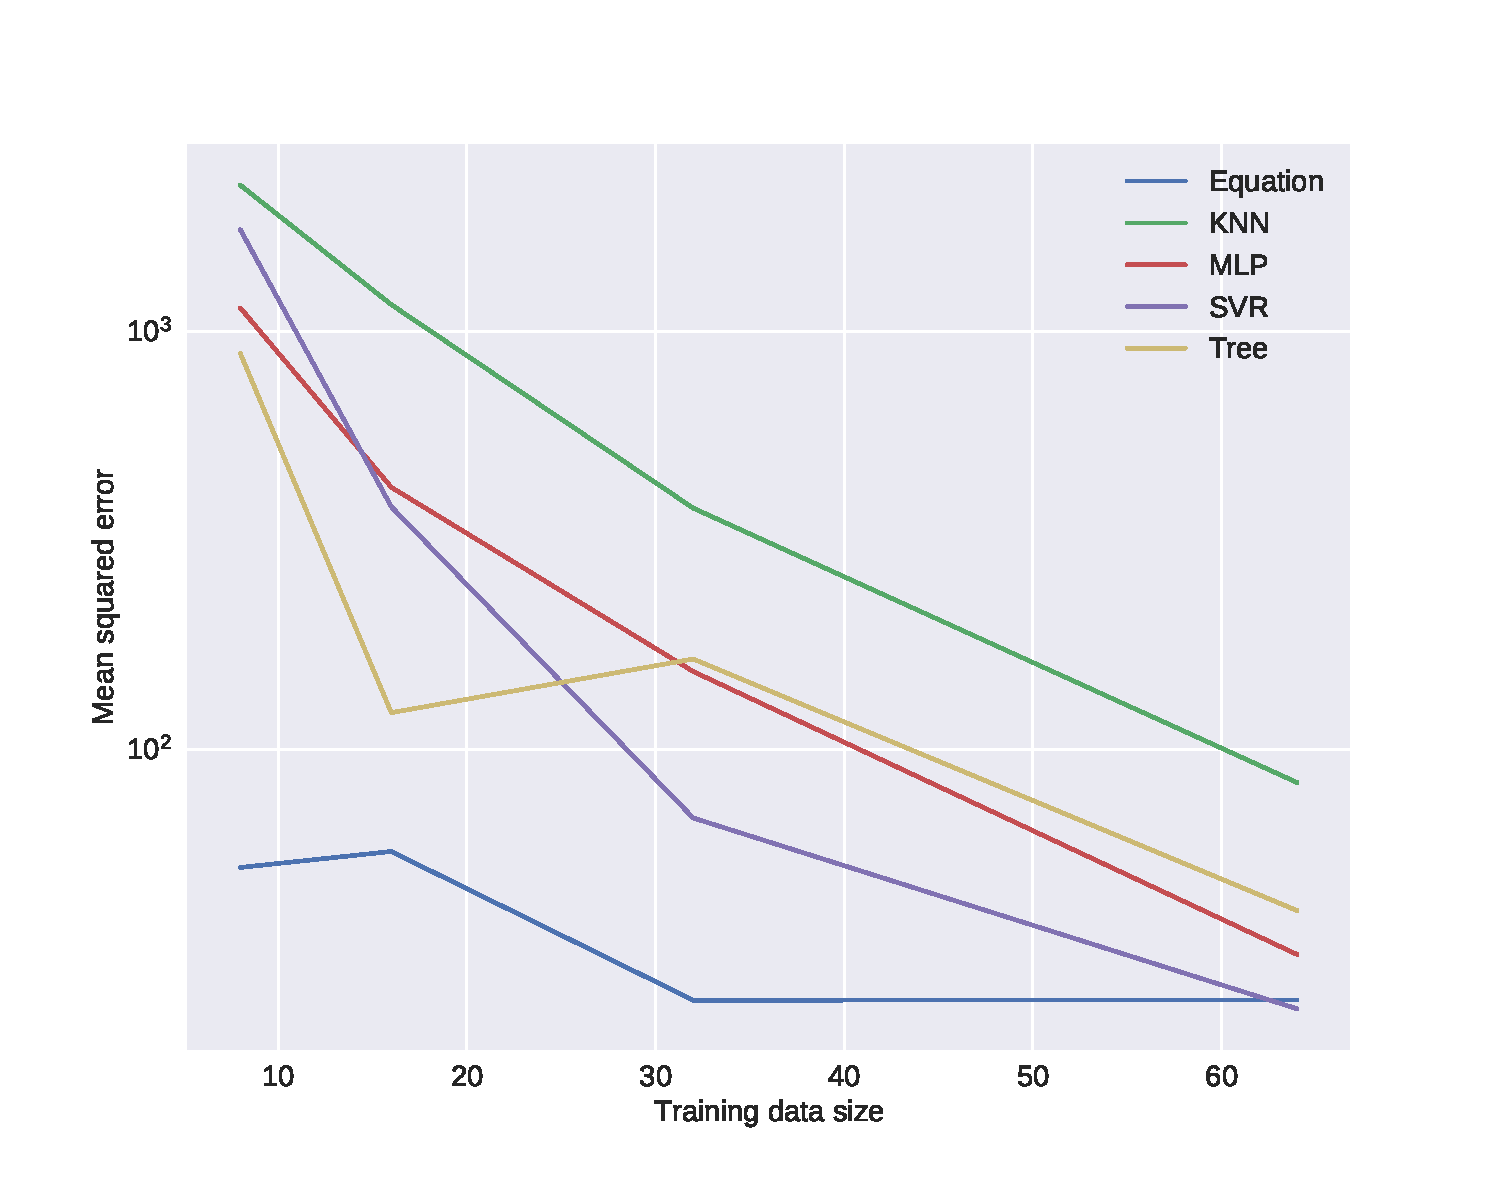
\includegraphics[width=\columnwidth]{experiments/figures/ml_models.pdf}
	\caption{Average of the mean squared error for all applications of our study case Section \ref{sec:casestudyapplication}.}
	\label{fig:ml_models}
\end{figure}

\subsection{Verifying Hypothesis} \label{subsec:ev_verifying_hypothesis}

In this section, we validate whether the assumptions of our model are valid for the system used.

\subsection{Frequency and Voltage Relation} \label{subsec:ev_frequency_and_voltage Relation}
One of the assumptions was that the frequency and the voltage have a linear relationship, as indicated by ~\cref{eq:f_v}. To verify that, we build an experiment that sets the frequency to a specific value while sampling the voltage using the APERF and MPERF registers that provide feedback on the current CPU frequency. The average result of the sampling voltages is shown in  \cref{fig:freq_volt_rel}, where we can observe a near-perfect linear relation. This is because manufacturers implement this curve in the processors, using tables that relate ranges of frequencies to voltages so that they can precisely define any curve that will better suit their design.

\begin{figure}[H]
	\centering
	\captionsetup[subfigure]{justification=centering}
	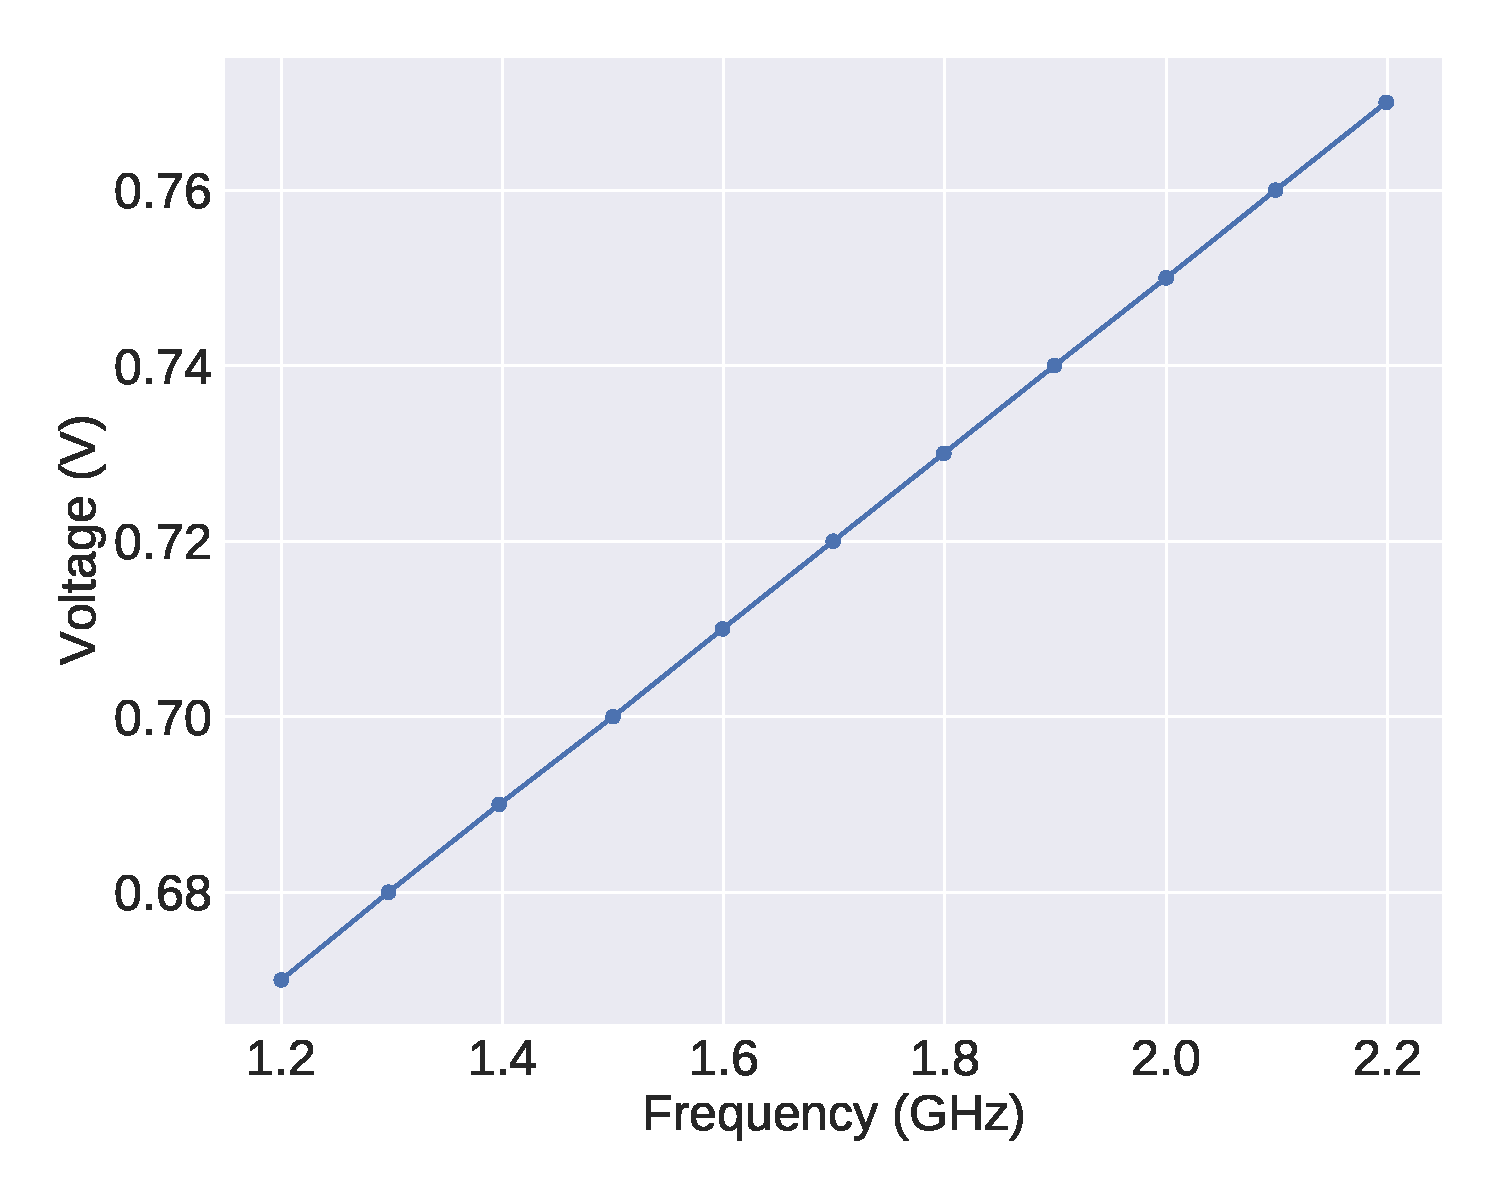
\includegraphics[width=\columnwidth]{experiments/figures/freq_volt_rel.pdf}
	\caption{Frequency voltage relation.}
	\label{fig:freq_volt_rel}
\end{figure}

\subsection{Input Size and Instructions} \label{subsec:ev_input_size_and_instructions}
We ran the applications with different inputs assuming  linear growth in the amount of work for one input to the other when building our model. However, measuring and controlling the amount of work would require much instrumentation and tuning to find an input corresponding to a certain amount of work. Therefore, to build our models, we use the time to reference the amount of work, assuming that the work is proportional to the executing time. \cref{fig:time_input} corresponds to the verification of this supposition.


\cref{tab:corr_in_time} shows that the assumption was reasonable since the average correlation was 0.96 for all applications, indicating that growth in the number of instructions  will follow the time. This was the case for all applications that we ran in our benchmark and should hold for any data parallelism type of application.
\begin{figure}[H]
	\centering
	\captionsetup[subfigure]{justification=centering}
	\begin{subfigure}[b]{0.45\textwidth}
		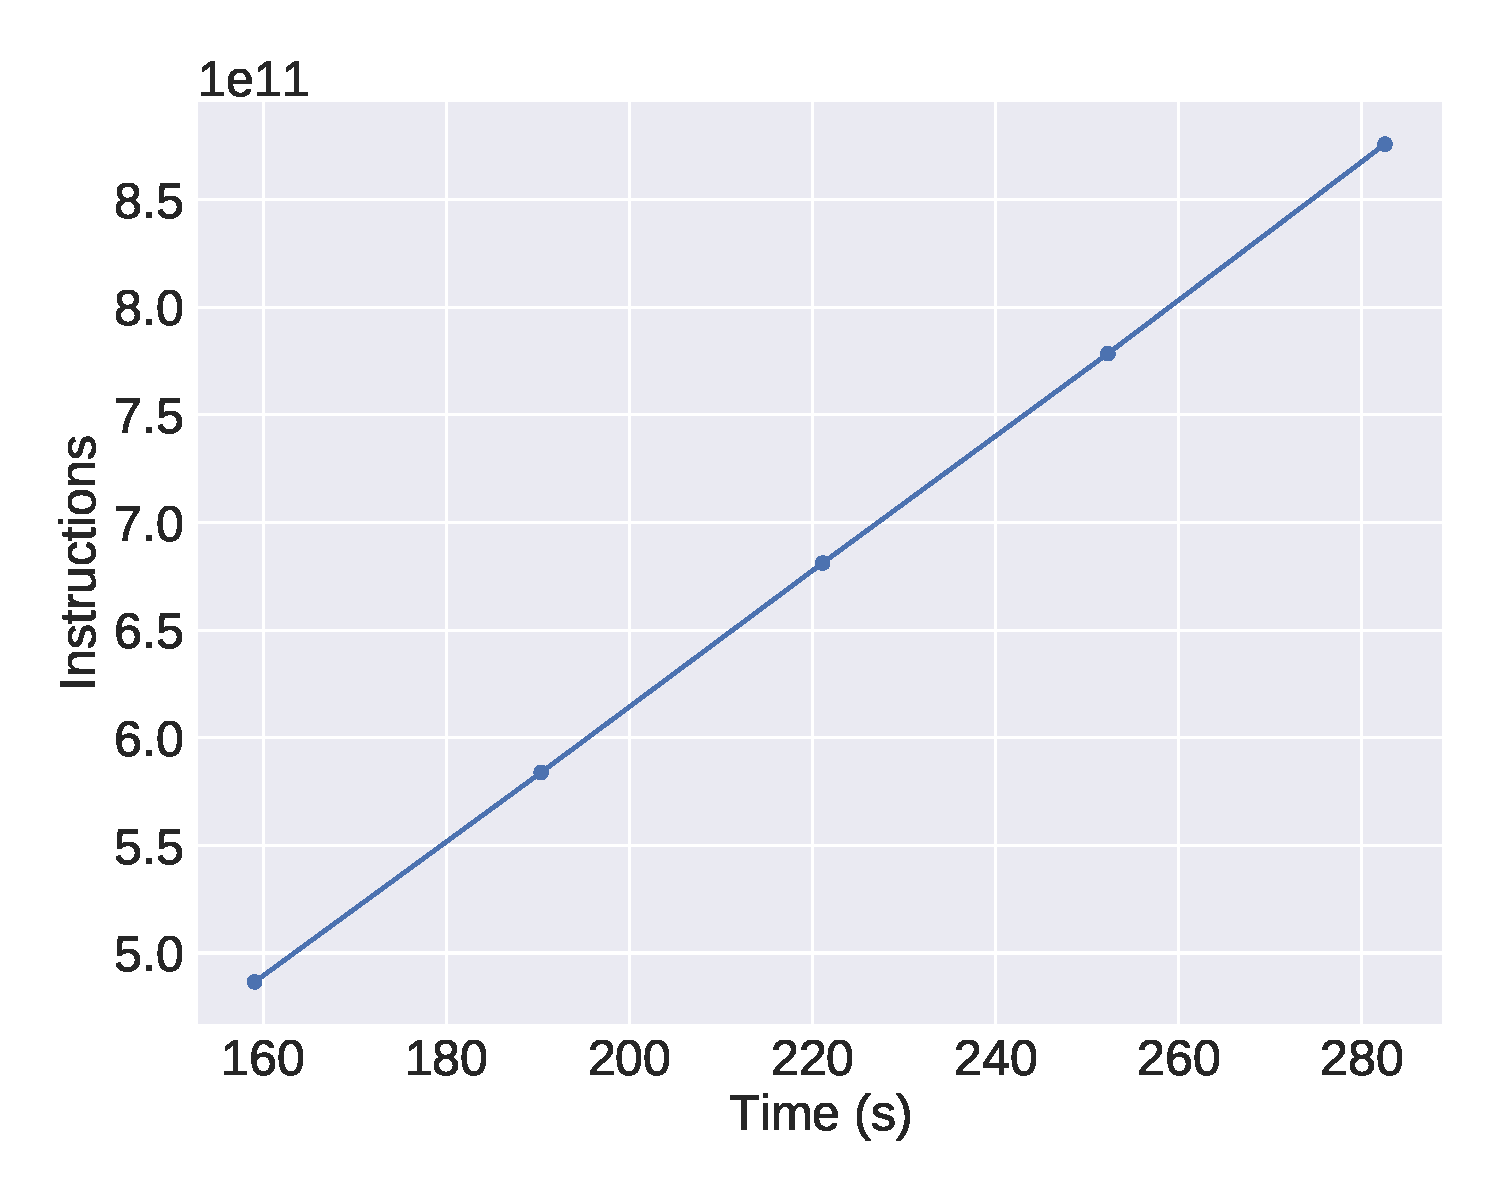
\includegraphics[width=\columnwidth]{models/figures/hypothesis/input_instructions/input_time/blackscholes.pdf}
		\caption{Blackscholes.}
		\label{fig:time_input_blackshoels}
	\end{subfigure}
	%
	\begin{subfigure}[b]{0.45\textwidth}
		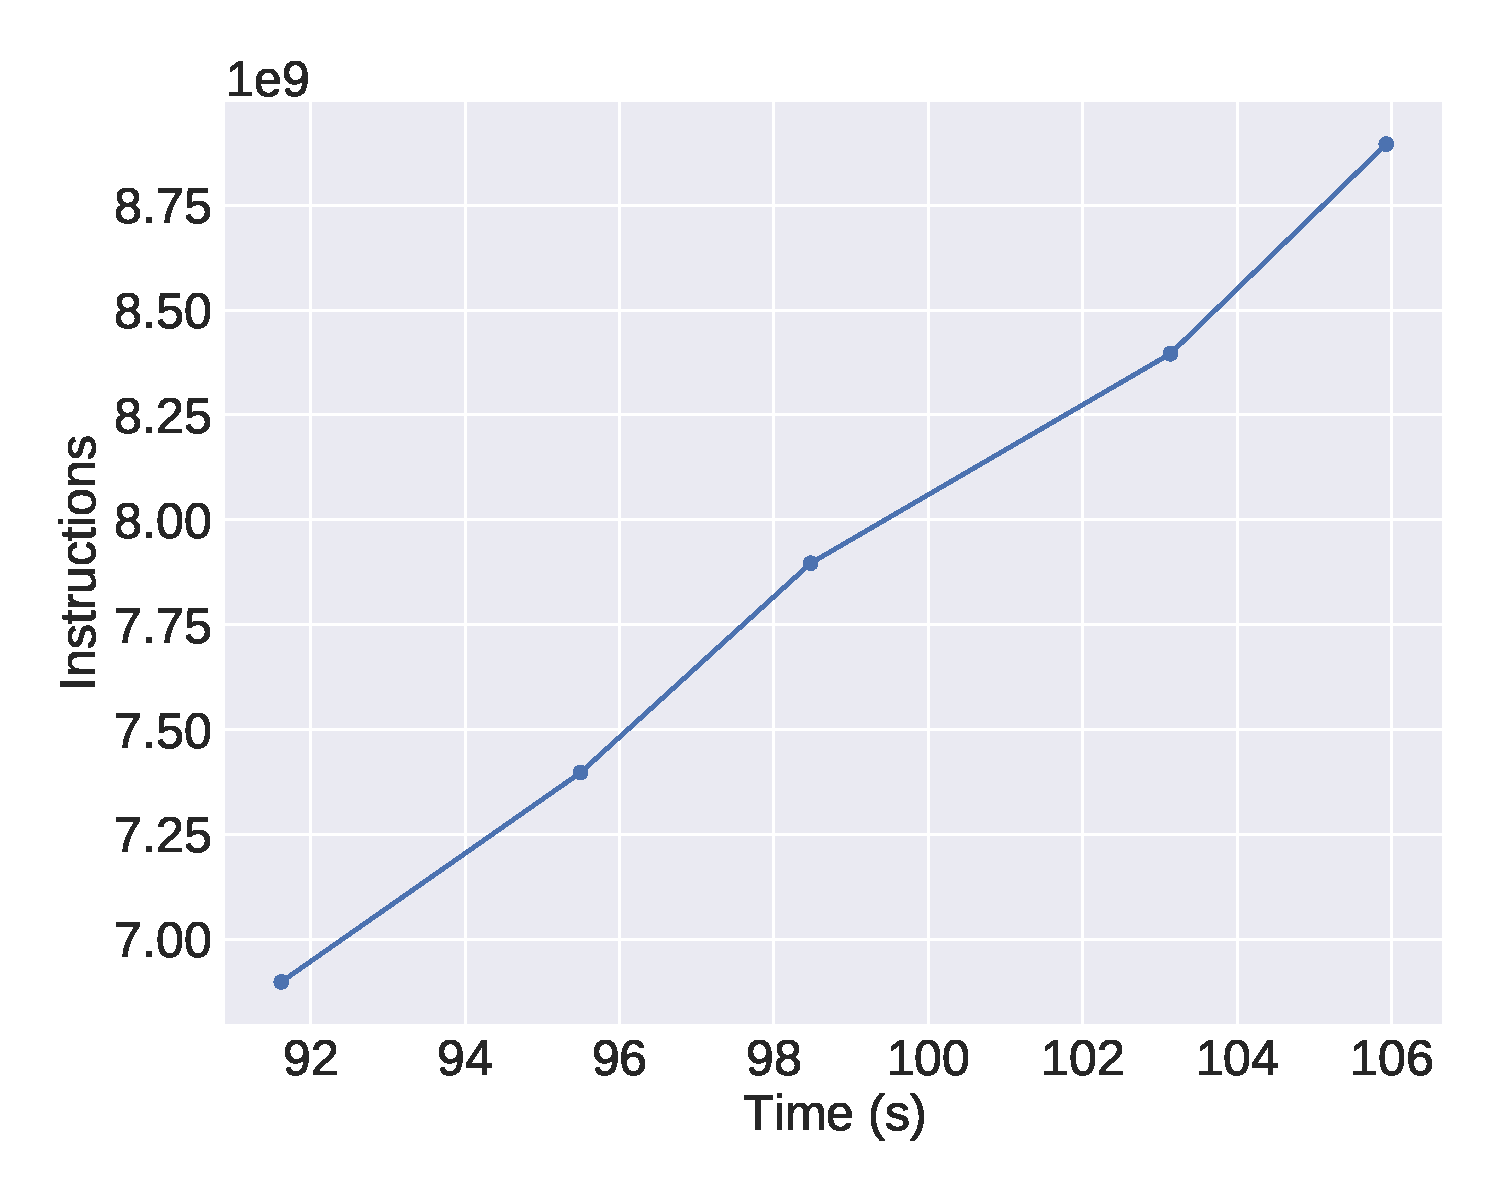
\includegraphics[width=\columnwidth]{models/figures/hypothesis/input_instructions/input_time/canneal.pdf}
		\caption{Canneal.}
		\label{fig:time_input_canneal}
	\end{subfigure}
	
	\hfill
	\caption{Relation between time and instructions for each input size. }
	\label{fig:time_input}
\end{figure}
\vspace{-6pt}

\begin{table}[H]
	\centering
	\caption{Correlation of time and instructions for all applications.}
	\begin{tabular}{ll}
		\multicolumn{1}{l|}{\textbf{Application}} & \textbf{Correlation} \\ \hline
		Blackscholes                                               & 0.99                                  \\
		Bodytrack                                                  & 0.99                                  \\
		Canneal                                                    & 0.99                                  \\
		Dedup                                                      & 0.99                                  \\
		Ferret                                                     & 0.96                                  \\
		Fluidanimate                                               & 0.99                                  \\
		Freqmineq                                                  & 0.99                                  \\
		Openmc                                                     & 0.94                                  \\
		Raytrace                                                   & 0.99                                  \\
		Swaptions                                                  & 0.99                                  \\
		Vips                                                       & 0.98                                  \\
		x264                                                       & 0.99                                  \\
		HPL                                                        & 0.79                                  \\ \hline
	\end{tabular}
	\label{tab:corr_in_time}
\end{table}

The next assumption was that the application's behavior was the same when varying the workload. This condition is necessary for using the model with an unknown input size because, if the behavior is the same, we can interpolate the known inputs. One way to verify this is to measure the rate of instructions per second normalized by the frequency, as shown in \cref{fig:fingerpritns}.
\begin{figure}[H]
	\centering
	\captionsetup[subfigure]{justification=centering}
	
	\begin{subfigure}[b]{0.45\textwidth}
		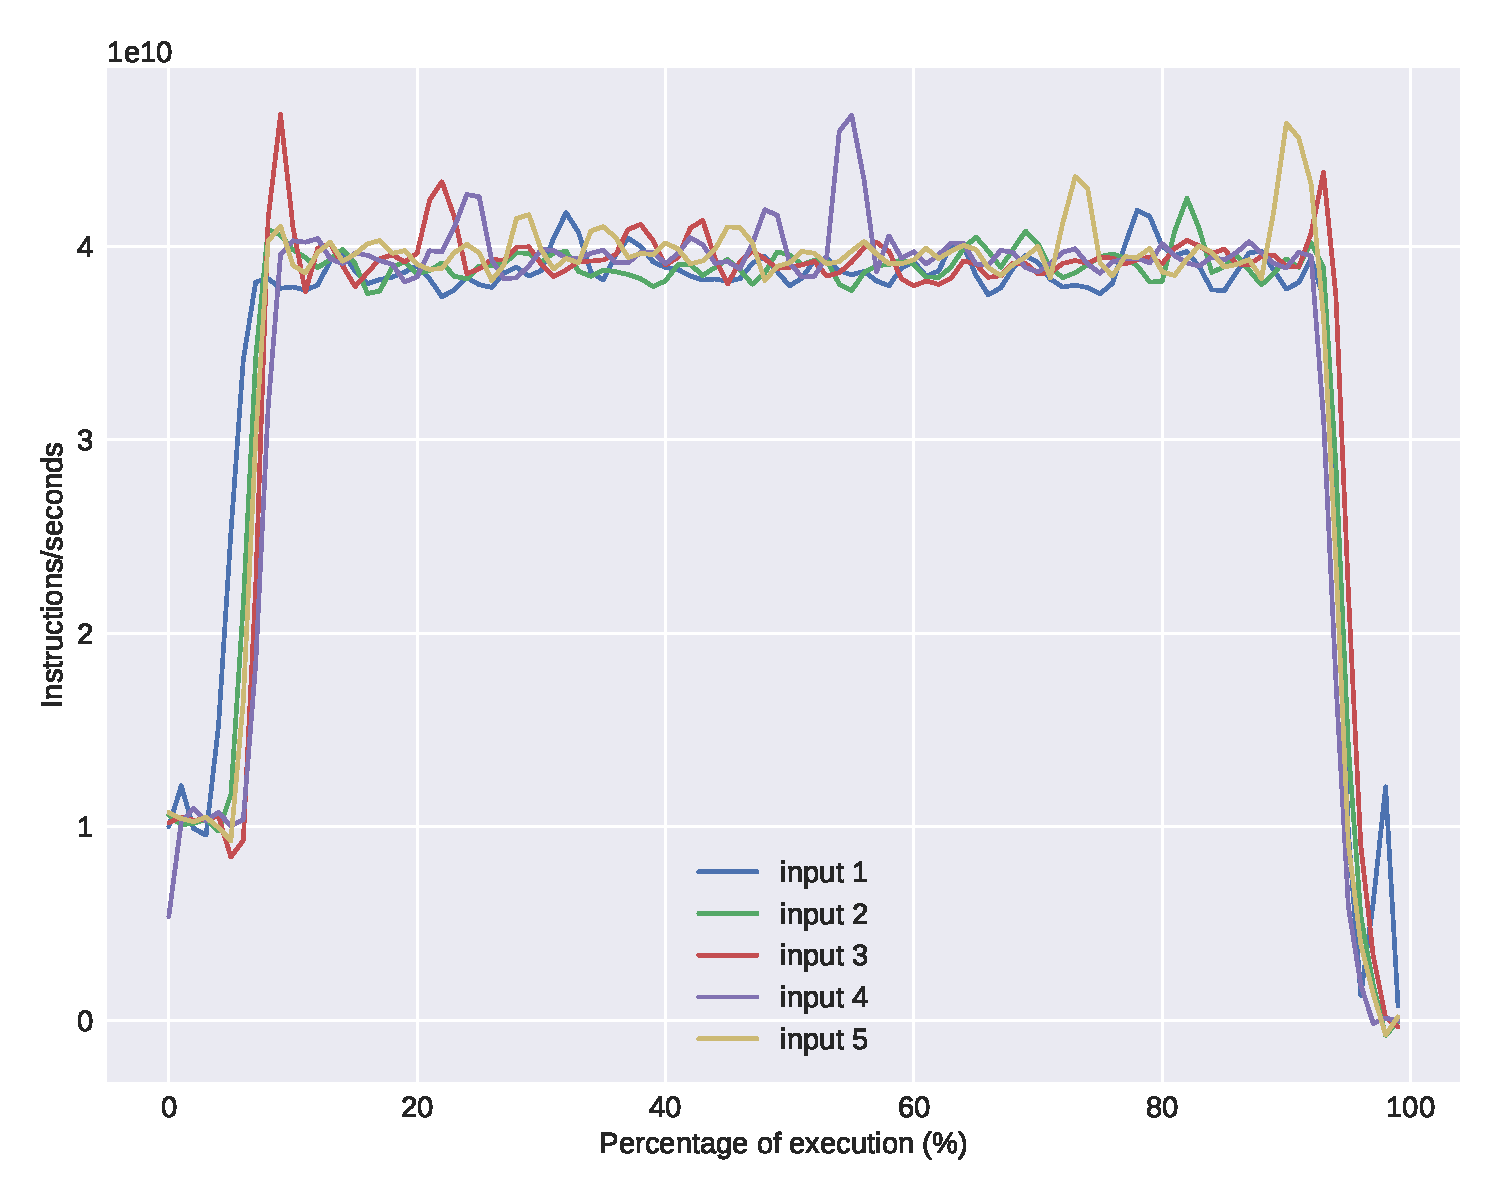
\includegraphics[width=\columnwidth]{models/figures/hypothesis/input_instructions/fp/blackscholes.pdf}
		\caption{Blacksholes.}
		\label{fig:fp_baclscholes}
	\end{subfigure}
	%
	\begin{subfigure}[b]{0.45\textwidth}
		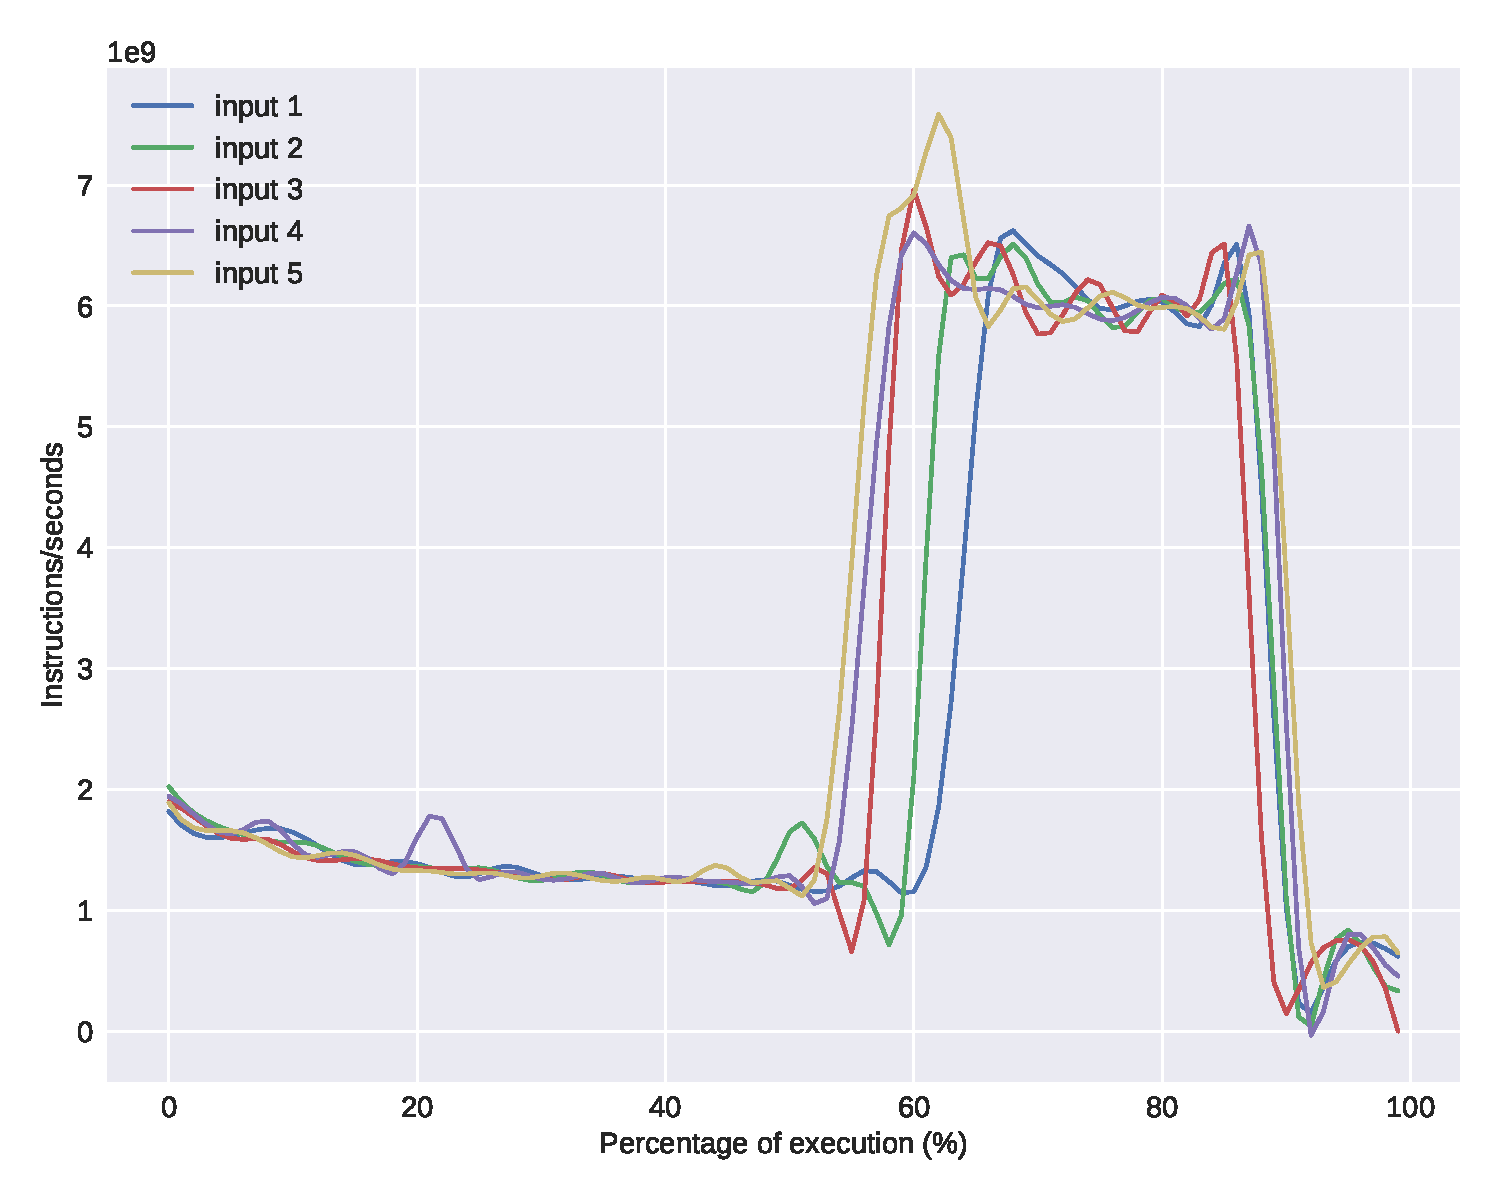
\includegraphics[width=\columnwidth]{models/figures/hypothesis/input_instructions/fp/canneal.pdf}
		\caption{Canneal.}
		\label{fig:fp_canneal}
	\end{subfigure}
	
	\hfill
	\caption{Rate of instructions per second varying the input size normalized by the frequency.}
	\label{fig:fingerpritns}
\end{figure}

\cref{fig:fingerpritns} shows that the applications have roughly the same curve when normalized; this also happens for all other applications in our benchmark.

The final assumption is that the workload should also not vary depending on the number of cores or frequency. To verify, we measure the total number of executed instructions while varying the cores from 1 to 32. \cref{tab:cores_variation} shows the results.

\begin{table}[H]
	\centering
	\caption{Variation of the number of instructions when changing the number of cores for the same input.}
	%\begin{tabular}{c|c|c|c}
	\begin{tabular*}{\hsize}{@{\extracolsep{\fill}}cccc}
		\toprule
		& \textbf{Average} & \textbf{Standard}     & \textbf{Standard}\\
		\multirow{-2}{*}{\textbf{Application}}& \textbf{Number of Instructions} & \textbf{Deviation}     & \textbf{Deviation} \textbf{(\%) }\\ \midrule
		Vip          & $7.97 \times 10^{11}$     & $7.16 \times 10^{6}$  & 0.00 \\ %Please use Scientific notation. For example, “1.65e+04” should be changed to “1.65× 104”. Please confirm `%` whether to remove.
		Openmc       & $8.17 \times 10^{7}$     & $ 1.65 \times 10^{4}$ & 0.02    \\ 
		Rtview       & $9.91 \times 10^{12}$     & $ 1.55 \times 10^{9}$ & 0.02    \\ 
		X264         & $4.52 \times 10^{11}$     & $ 5.81 \times 10^{7}$ & 0.01    \\ 
		Bodytrack    & $1.86 \times 10^{12}$     & $ 3.95 \times 10^{10}$ & 2.13    \\ 
		Fluidanimate & $2.09 \times 10^{12}$     & $ 8.44 \times 10^{10}$ & 4.04    \\ 
		HPL          & $1.14 \times 10^{8}$      & $ 1.24 \times 10^{5}$ & 0.11    \\ 
		Blackschole  & $3.75 \times 10^{12}$     & $ 1.40 \times 10^{9}$ & 0.04     \\ 
		Dedup        & $1.02 \times 10^{11}$     & $ 5.74 \times 10^{7}$ & 0.06     \\ 
		Swapti       & $2.43 \times 10^{12}$     & $ 8.87 \times 10^{8}$ & 0.04     \\ 
		Canneal      & $1.19 \times 10^{11}$     & $ 4.46 \times 10^{7}$ & 0.04     \\ 
		Freqmine     & $1.27 \times 10^{12}$     & $ 4.78 \times 10^{8}$ & 0.04     \\ 
		Ferret       & $4.76 \times 10^{11}$     & $ 7.04 \times 10^{7}$ & 0.01     \\ \bottomrule
	\end{tabular*}
	\label{tab:cores_variation}
\end{table}
% Corrected

\cref{tab:cores_variation} shows the standard deviation and what that corresponds to in terms of the total number of instructions as a percentage. 

The same test was performed for the frequency, varying from 1.2 to 2.2 GHz with 100~MHz steps. The results are shown in \cref{tab:freq_variation}.

These results show that all the assumptions were reasonable, and we can safely move to the validation of the model's prediction.
\begin{table}[H]
	\caption{Variation of the number of instructions when changing the frequency for the same input.}
	\centering
	%\begin{tabular}{c|c|c|c}{\hsize}{@{\extracolsep{\fill}}cccc}
	\begin{tabular*}{\hsize}{@{\extracolsep{\fill}}cccc}
		\toprule
		& \textbf{Average} & \textbf{Standard}     & \textbf{Standard}\\
		\multirow{-2}{*}{\textbf{Application}}& \textbf{Number of Instructions} & \textbf{Deviation}     & \textbf{Deviation} \textbf{(\%)} \\ \midrule
		Vip          & $7.97 \times 10^{11}$      & $ 1.16 \times 10^{6}$  & 0.00      \\ 
		Openmc       & $8.17 \times 10^{7}$       & $ 4.52 \times 10^{3}$  & 0.01      \\ 
		Rtview       & $9.91 \times 10^{12}$      & $ 6.64 \times 10^{5}$  & 0.00      \\ 
		X264         & $4.52 \times 10^{11}$      & $ 1.54 \times 10^{5}$  & 0.00      \\ 
		Bodytrack    & $1.84 \times 10^{12}$      & $ 2.54 \times 10^{5}$  & 0.00      \\ 
		Fluidanimate & $2.38 \times 10^{12}$      & $ 1.70 \times 10^{9}$  & 0.07      \\ 
		HPL          & $1.14 \times 10^{8}$       & $ 5.95 \times 10^{3}$  & 0.01      \\ 
		Blackschole  & $3.75 \times 10^{12}$      & $ 4.36 \times 10^{5}$  & 0.00      \\ 
		Dedup        & $1.02 \times 10^{11}$      & $ 8.32 \times 10^{7}$  & 0.08      \\ 
		Swapti       & $2.43 \times 10^{12}$      & $ 1.48 \times 10^{5}$  & 0.00      \\ 
		Canneal      & $1.19 \times 10^{11}$      & $ 3.01 \times 10^{5}$  & 0.00      \\ 
		Freqmine     & $1.27 \times 10^{12}$      & $ 3.70 \times 10^{8}$  & 0.03      \\ 
		Ferret       & $4.76 \times 10^{11}$      & $ 5.63 \times 10^{7}$  & 0.01      \\\bottomrule
	\end{tabular*}
	\label{tab:freq_variation}
\end{table}


\section{Fitting the Models} \label{subsec:fitting_the_models}
To find the parameters of  \cref{eq:en_final}, 10 uniformly random configurations of frequencies ($f$), cores ($p$) and inputs ($N$) were chosen from the range $1<=p<=32$, $1.2<=f<=2.2$ and $1<=N<=5$, respectively. The application was executed for each chosen configuration, and the measured energy and time values were collected. For the input size, if we assume that all CPU instructions take approximately the same time to execute, the number of basic operations will be directly correlated with the time. Thus, we can estimate the input size by looking at the execution time, allowing us to divide a large input size into several smaller ones, knowing their relationship, as performed in the work of Oliveira ~\cite{Oliveira2018ApplicationCharacterization}. The unity can also vary depending on the definition. For simplicity, we assign numbers from 1 to 10, increasing the problem linearly, so it is also possible to interpolate any input in between these values.

For each configuration, samples of the power were collected using IPMI every 1 second. This sampling rate was chosen based on the magnitude of the mean run time of the applications, which is in the order of minutes. Therefore, this rate provides enough samples to measure average power. Additionally, timestamps and the total run time were collected. The total energy spent on each configuration is estimated by first interpolating the power samples using the first-order method and then integrating this function in the time.

The model's parameters are calculated by solving an optimization problem of finding the values that minimize the squared error of the prediction to the measured values using the non-linear least-squares method.

The Python library Scikit-Learn was used to build the SVR model~\cite{Pedregosa2011Scikit-learn:Python}. The SVR was trained using the same data used for parameter estimation of Equation (\ref{eq:en_final}) %\cref{eq:en_final}
with a grid search used to find the best kernel function and the best values for the hyper-parameters penalty for the wrong ($C$) and ($\gamma$). For this data, the best function was the radial base function (RBF), and the hyper-parameters were $C=10^4$ and $\gamma=0.5$.


\section{Measured versus Modeled Energy} \label{sec:measured_versus_modeled_energy}

To validate the model, we ran all possible configurations in the tested machine, varying the cores in a range of $1<=p<=32$, the frequency in $1.2<=f<=2.2$, and the input in $1<=N<=5$. The total number of configurations varies from 400 to over 1000 depending on the application, as some applications have restrictions on the number of cores that they can run. Once the data was collected, we computed the mean percentage error (MPE) according to the following equation:
\begin{equation}
	MPE = \frac{1}{N} \sum_i^N \frac{|y_{\rm estimated}-y_{\rm measured}|}{y_{\rm measured}}.
	\label{eq:mpe}
\end{equation}

\subsection{Frequency $\times$ Cores} \label{subsec:mvme_frequency_x_cores}
\cref{fig:en_eq_freq_cores_fc} plots the measured and modeled energy consumption for some of the applications modeled. In addition,  some of the possible shapes that the model can take while varying the number of active cores, and operating frequency, are shown.%please confirm that the intended meaning has been retained.
% yes its the same

\begin{figure}[H]
	\centering
	\captionsetup[subfigure]{justification=centering}
	\begin{subfigure}[b]{0.45\textwidth}
		\centerline{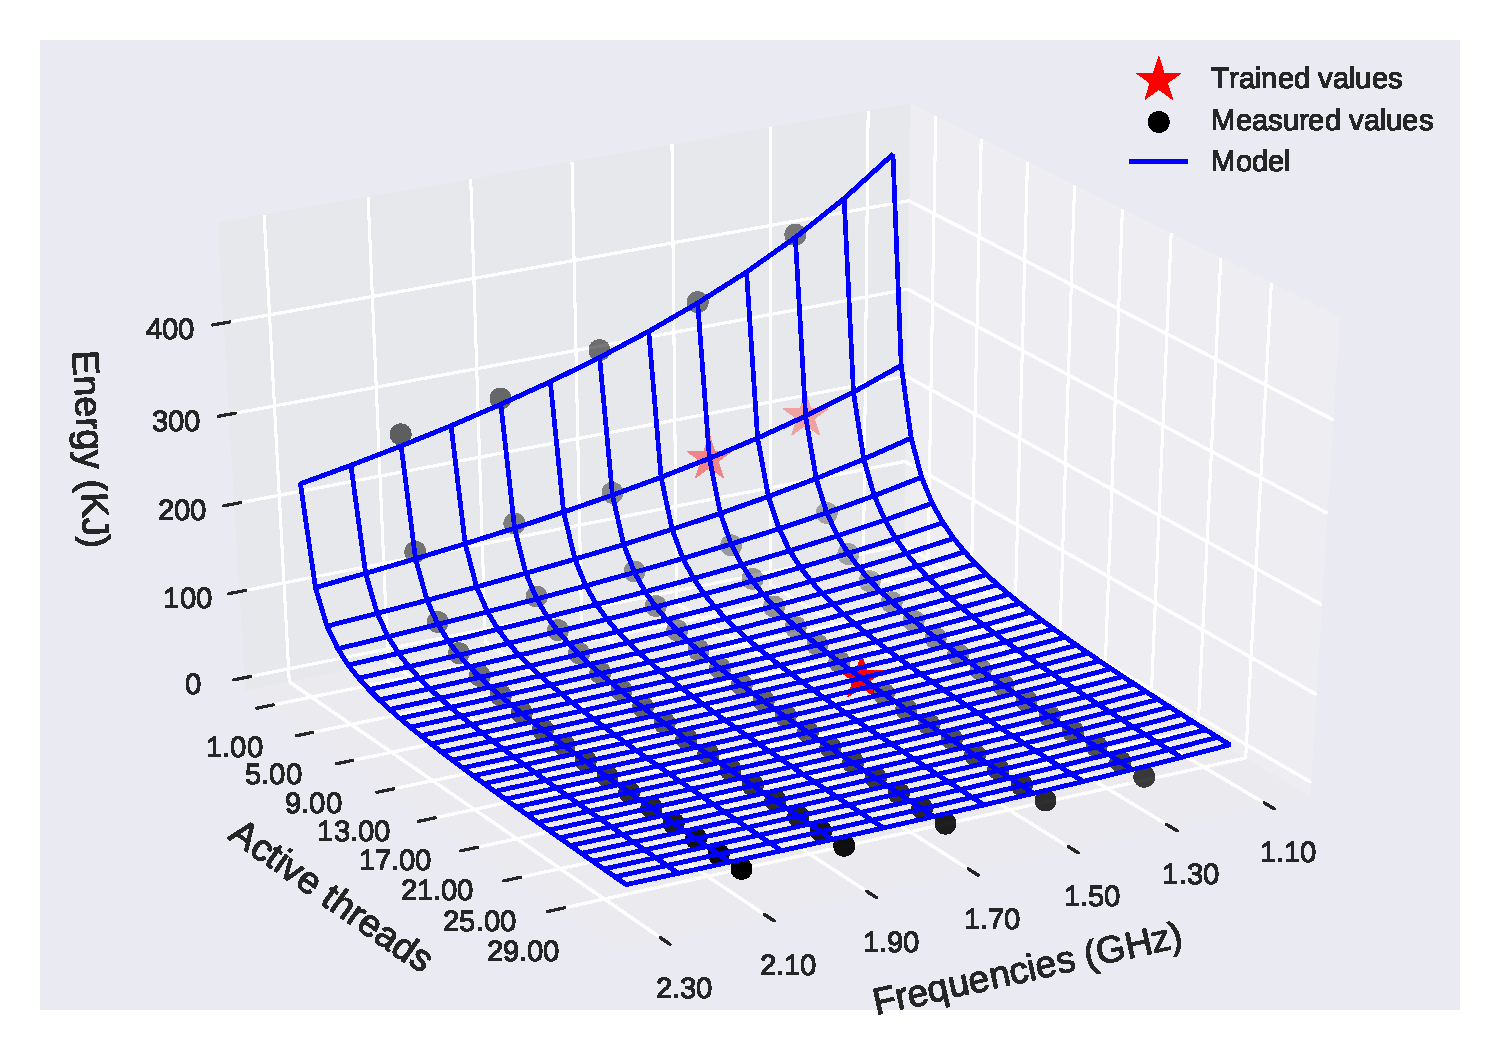
\includegraphics[width=\columnwidth]{models/figures/energy/freq_cores/completo_black_5.pdf}}
		\caption{}
		\label{fig:en_eq_black_fc}
	\end{subfigure}
	%
	\begin{subfigure}[b]{0.45\textwidth}
		\centerline{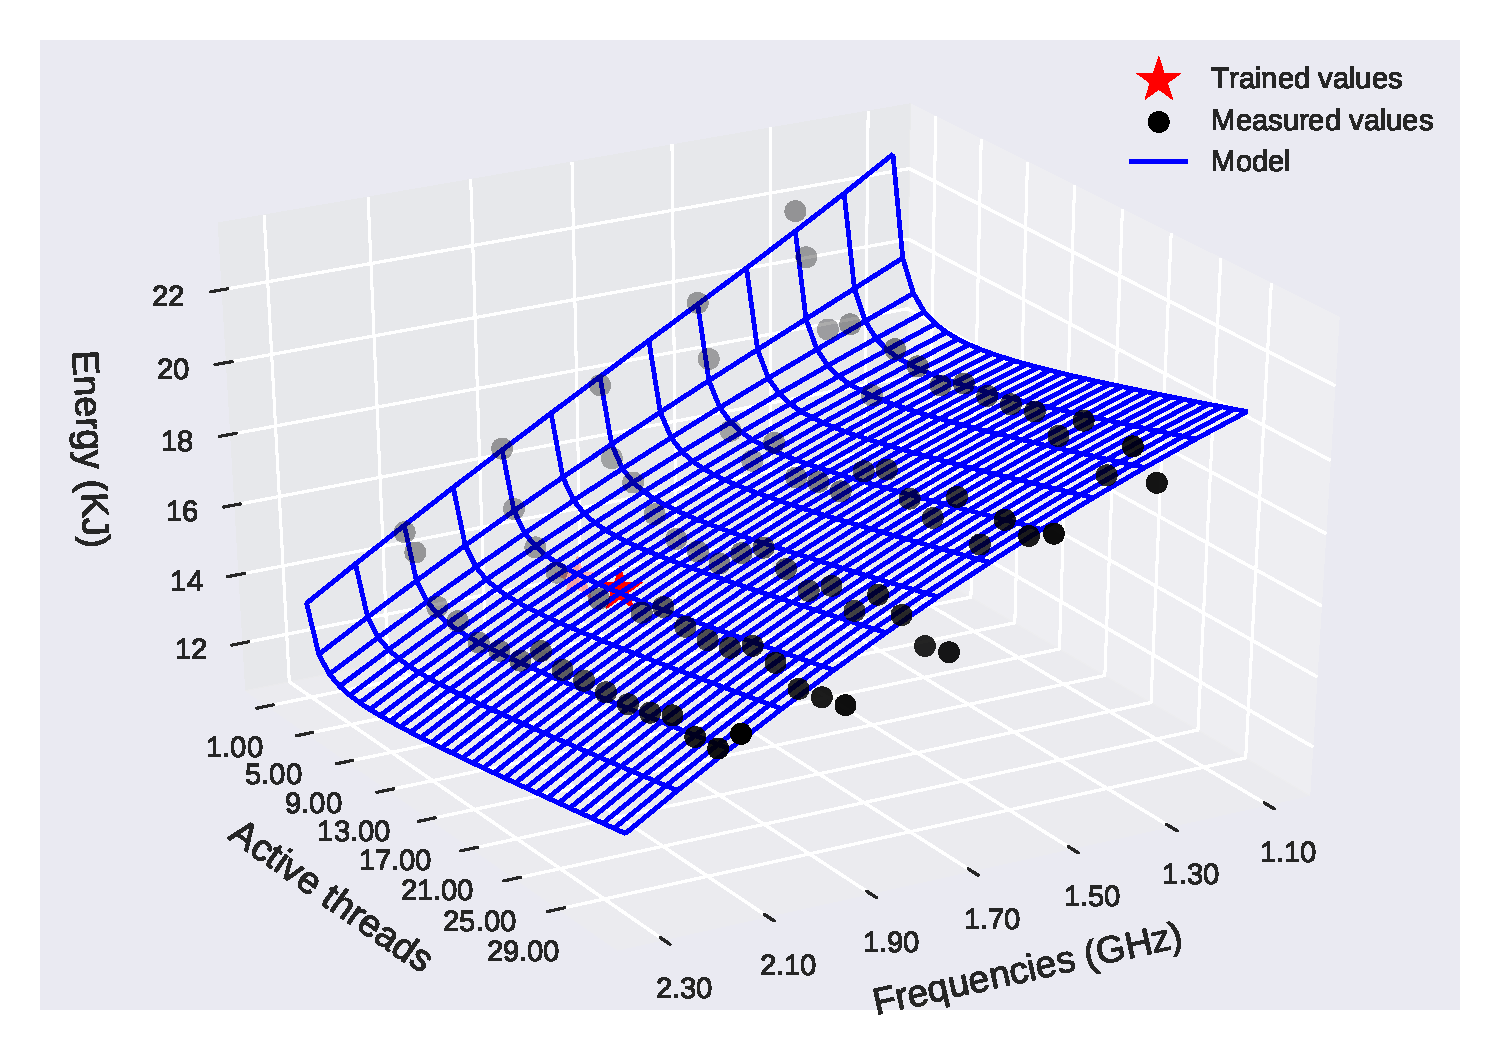
\includegraphics[width=\columnwidth]{models/figures/energy/freq_cores/completo_canneal_1.pdf}}
		\caption{}
		\label{fig:en_eq_canneal_fc}
	\end{subfigure}
	
	\caption{Example fit for a specific input size: Blackscholes (\textbf{a}) and Canneal (\textbf{b}).  “measured values” are the sensor data, and “minimum energy” is the minimum energy model prediction.
	}
	\label{fig:en_eq_freq_cores_fc}
\end{figure}

\subsection{Frequency $\times$ Input} \label{subsec:mvme_frequency_x_input}
\cref{fig:en_eq_freq_inp_fi} plots the measured and modeled energy consumption for some of the applications modeled. The diagrams show some of the possible shapes that the model can take while varying the operating frequency, and input size.
\begin{figure}[H]
	\centering
	\captionsetup[subfigure]{justification=centering}
	\begin{subfigure}[b]{0.45\textwidth}
		\centerline{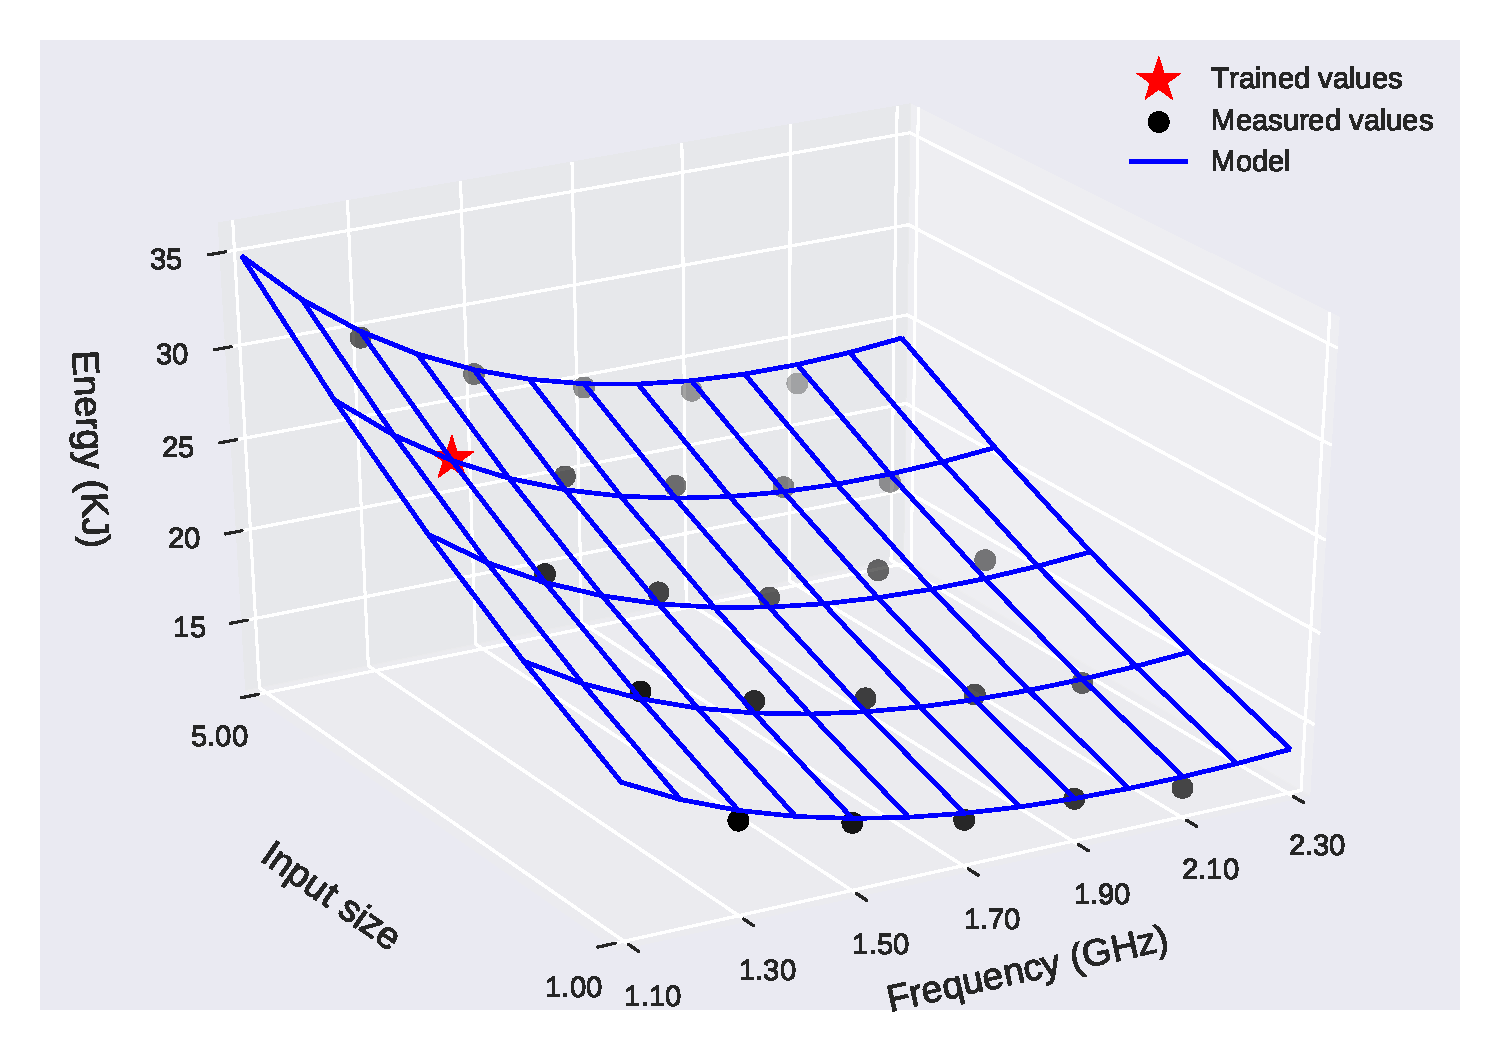
\includegraphics[width=\columnwidth]{models/figures/energy/freq_inps/completo_black_5.pdf}}
		\caption{}
		\label{fig:en_eq_black_fi}
	\end{subfigure}
	%
	\begin{subfigure}[b]{0.45\textwidth}
		\centerline{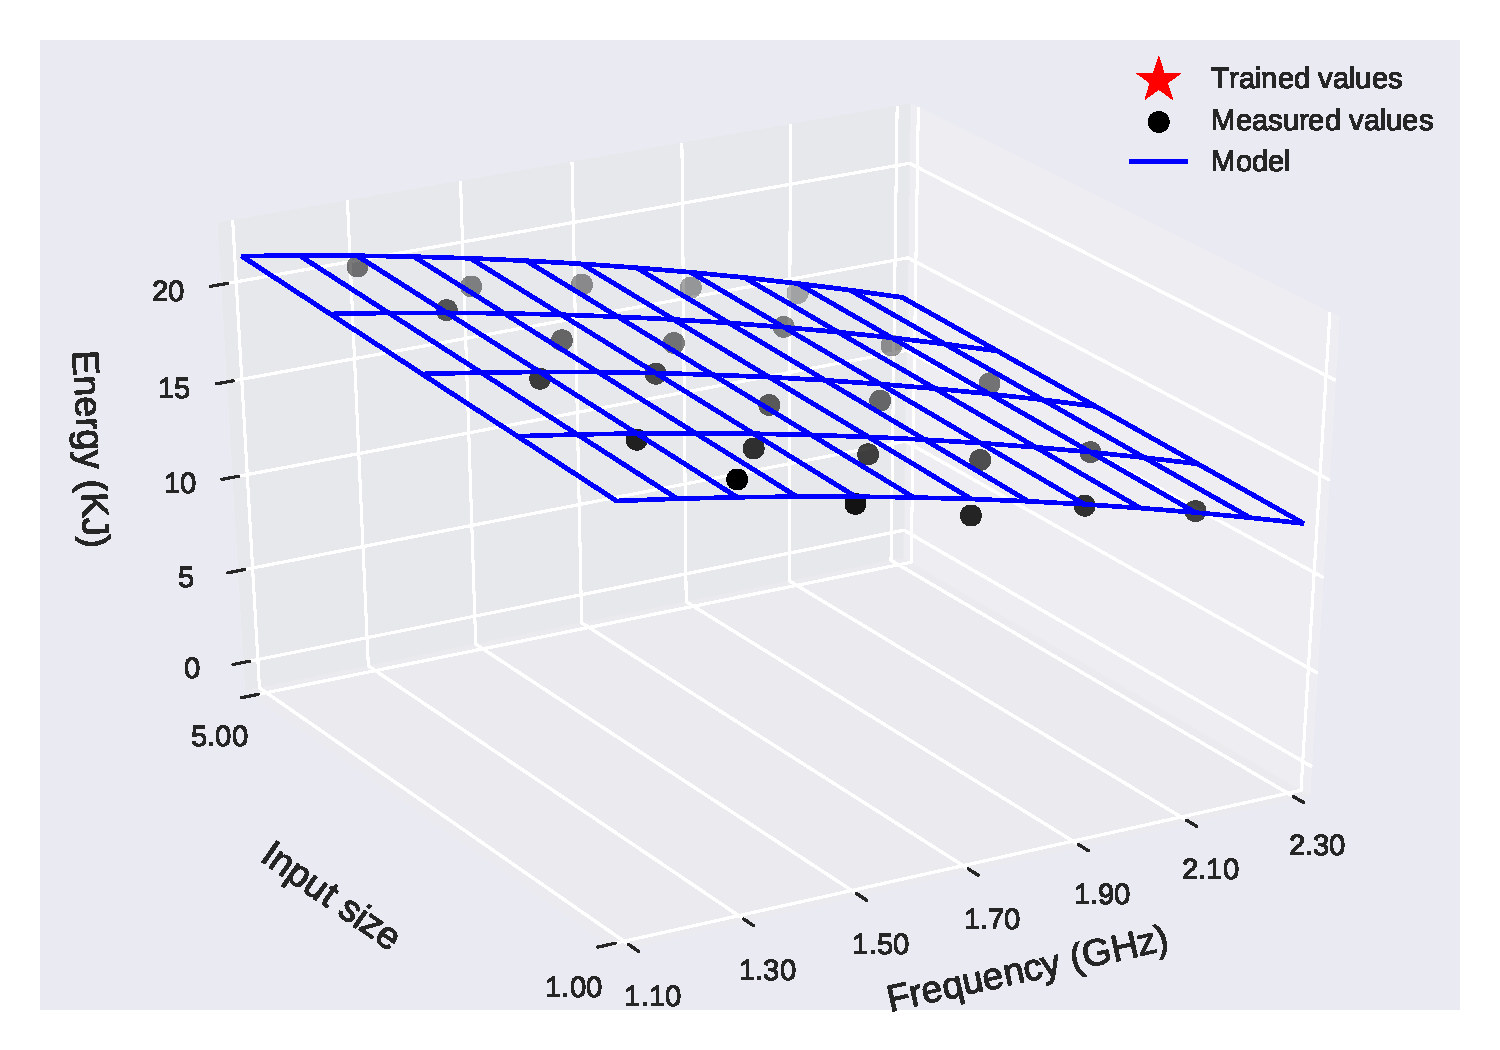
\includegraphics[width=\columnwidth]{models/figures/energy/freq_inps/completo_canneal_1.pdf}}
		\caption{}
		\label{fig:en_eq_canneal_fi}
	\end{subfigure}
	
	\caption{Example fit for a specific input size: Blackscholes (\textbf{a}) and Canneal (\textbf{b}).  “measured values” are the sensor data and “minimum energy” is the minimum energy model prediction.
	}
	\label{fig:en_eq_freq_inp_fi}
\end{figure}

\subsection{Cores $\times$ Input} \label{subsec:mvme_cores_x_input}
\cref{fig:en_eq_core_inp_ci} plots the measured and modeled energy consumption for some of the applications modeled. The diagrams  show some of the possible shapes that the model can take while varying the number of active cores, and input size.
\begin{figure}[H]
	\centering
	\captionsetup[subfigure]{justification=centering}
	\begin{subfigure}[b]{0.45\textwidth}
		\centerline{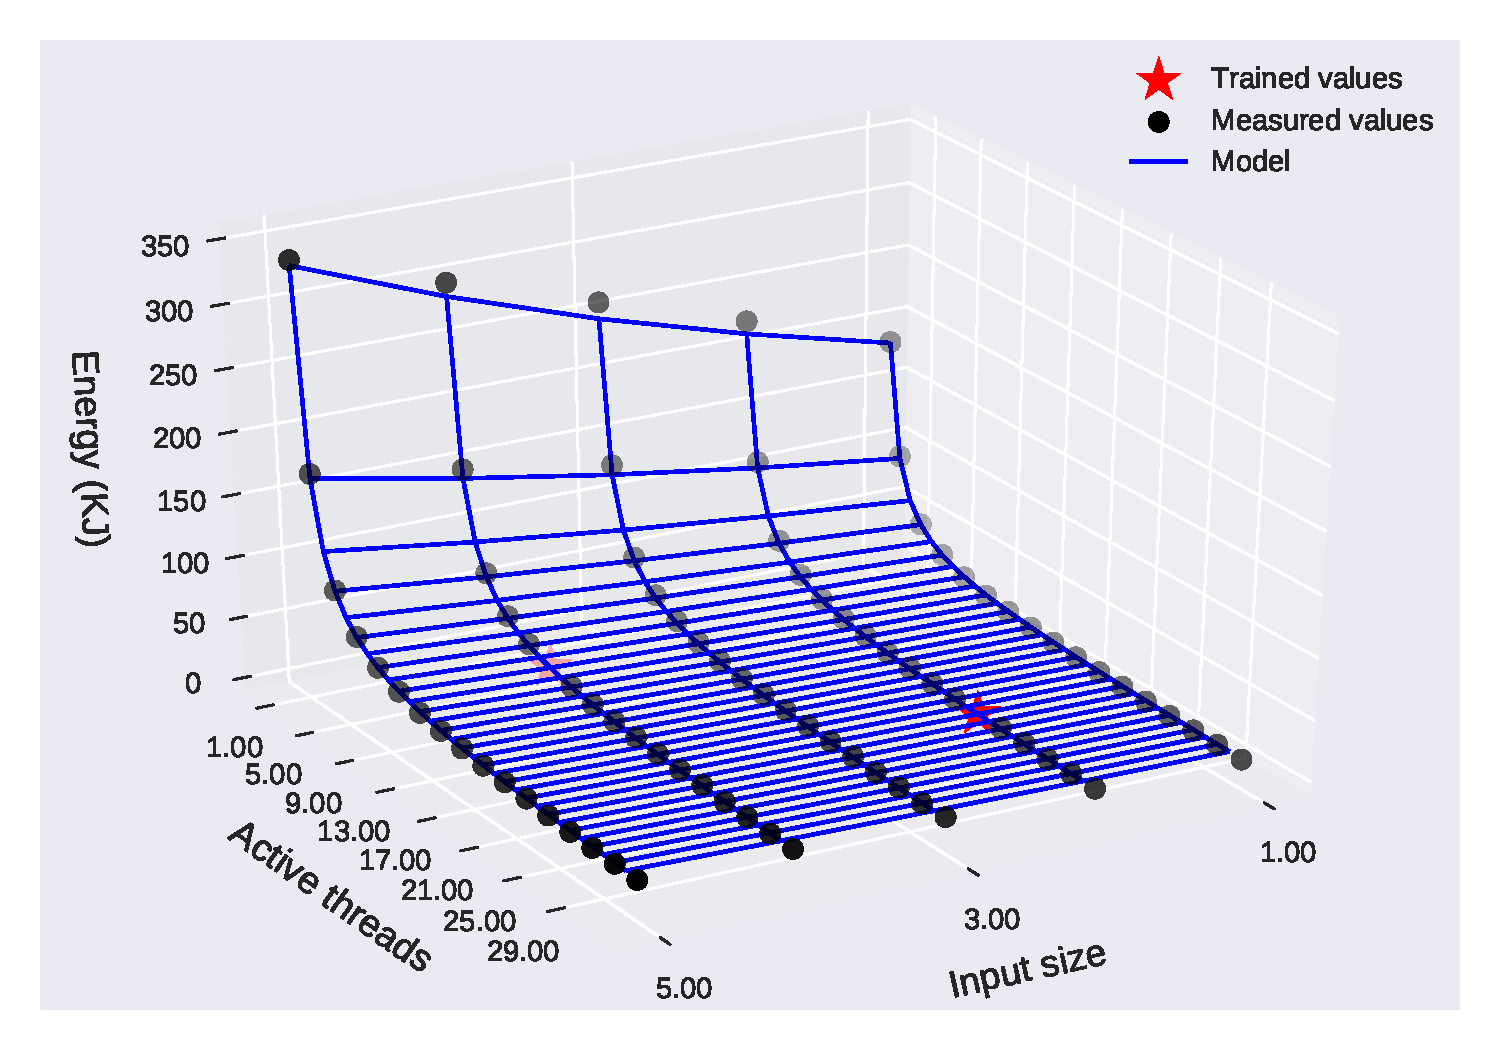
\includegraphics[width=\columnwidth]{models/figures/energy/cores_inps/completo_black_5.pdf}}
		\caption{}
		\label{fig:en_eq_black_ci}
	\end{subfigure}
	%
	\begin{subfigure}[b]{0.45\textwidth}
		\centerline{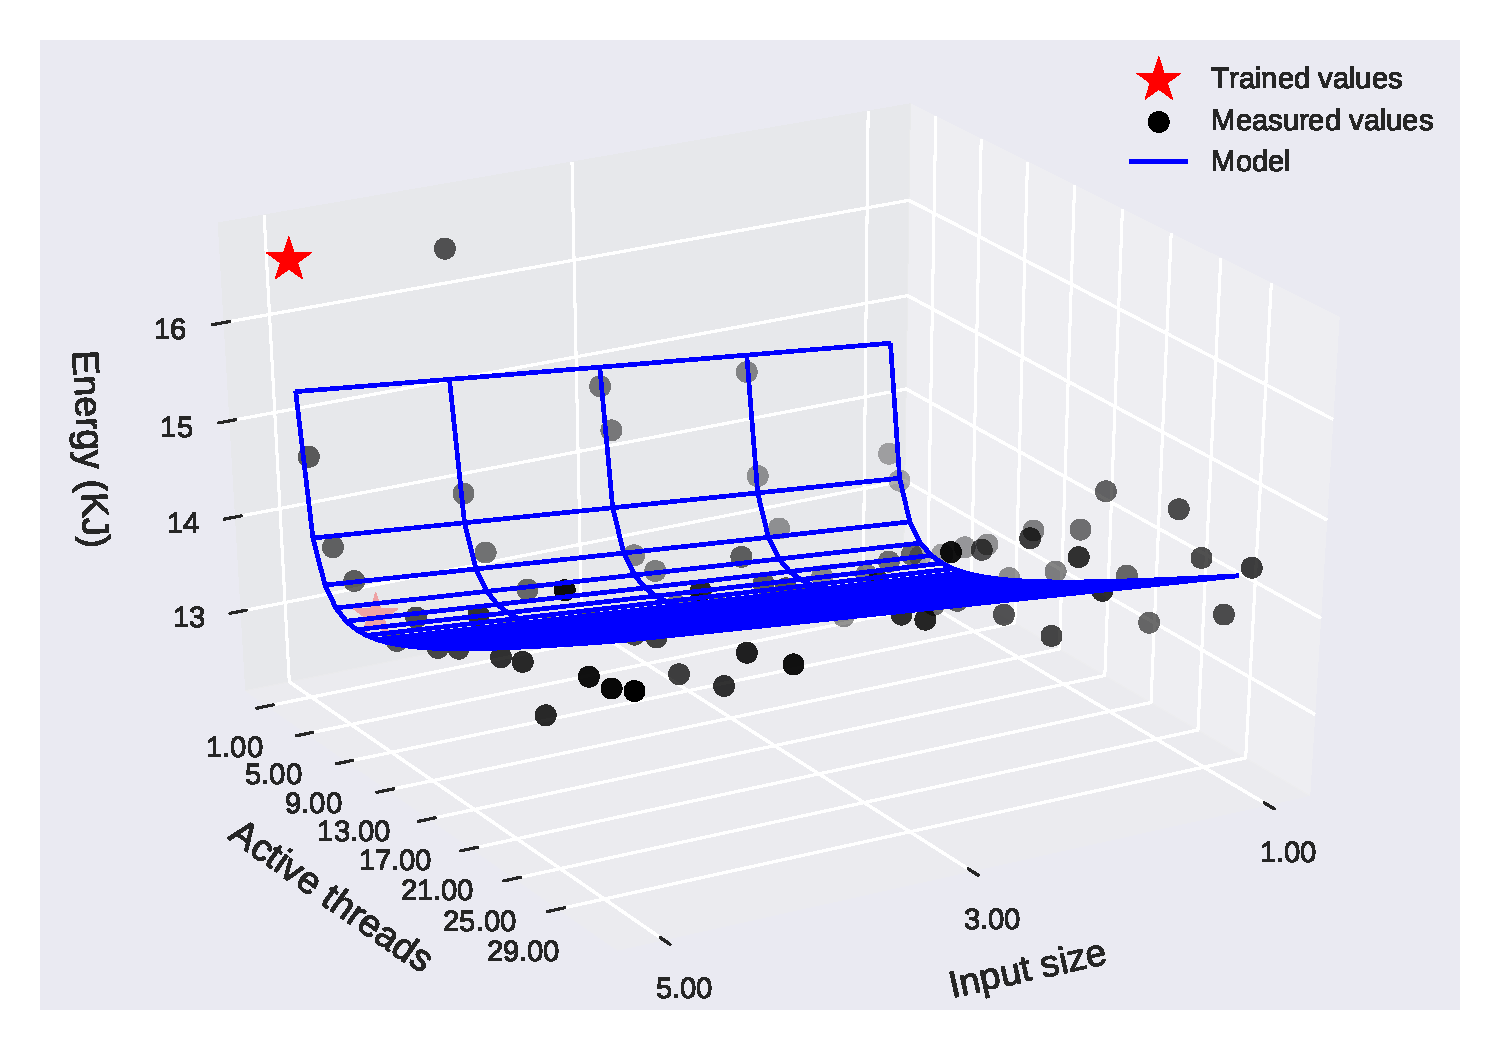
\includegraphics[width=\columnwidth]{models/figures/energy/cores_inps/completo_canneal_1.pdf}}
		\caption{}
		\label{fig:en_eq_canneal_ci}
	\end{subfigure}
	
	\caption{Example fit for a specific input size: Blackscholes (\textbf{a}) and Canneal (\textbf{b}).  “measured values” are the sensor data and “minimum energy” is the minimum energy model prediction.
	}
	\label{fig:en_eq_core_inp_ci}
\end{figure}


\section{Comparison} \label{sec:comparison}
The average results for each application were calculated using a model trained with only 10 configurations, and the comparison is displayed \cref{fig:mpe_svr_eq}. %We calculated the raw MPE values shown in ~\cref{tab:mpe_svr_eq}.
\begin{figure}[H]
	\centering
	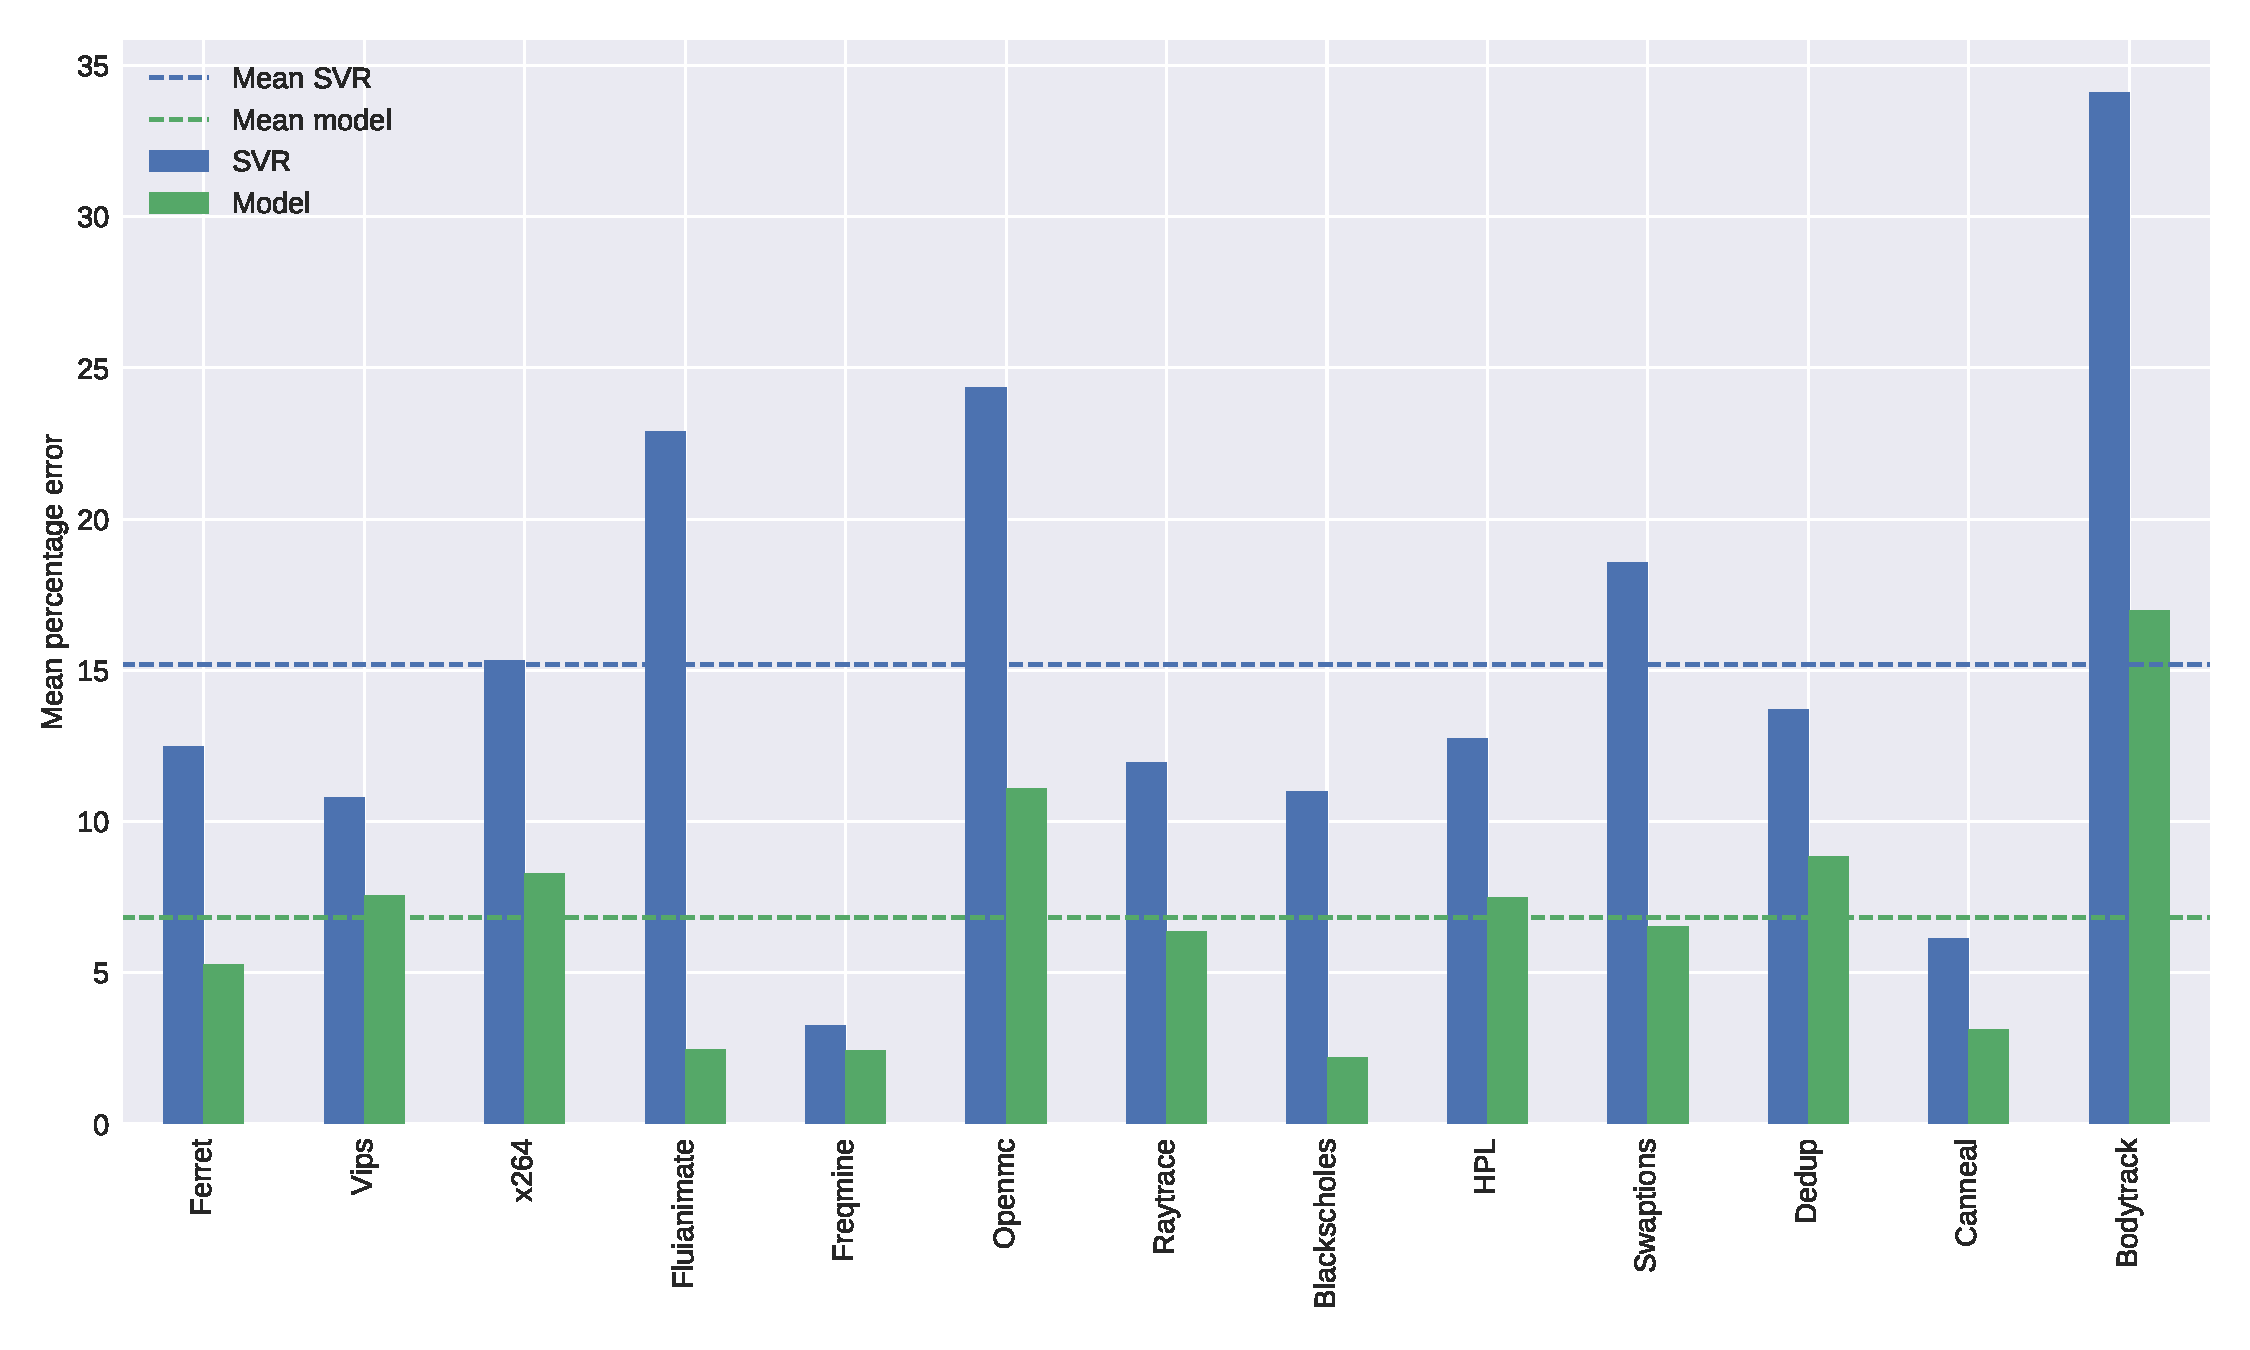
\includegraphics[width=.8\columnwidth]{models/figures/mpe_svr_eq.pdf}
	\caption{Comparison of the mean percentage error between the proposed model and SVR. ``Model mean'' and ``SVR mean'' are the average of all MPE values for all applications.
	}
	\label{fig:mpe_svr_eq}
\end{figure}

\cref{fig:mpe_svr_eq} shows that the proposed model always performed better, with a lower MPE than SVR, when we were limited to 10 training points. This result is further explored in the next Section \ref{sec:overhead_on_training}, where we undertake a comparison with different training sizes. The exact values are shown in \cref{tab:mpe_svr_eq}.

\begin{table}[H]
\centering
\begin{tabular}{c|c|c}
\hline
Application  & Model & SVR   \\ \hline
Ferret       & 5.25     & 12.49  \\ 
Raytrace     & 6.36     & 11.95  \\
Fluianimate  & 2.44     & 22.90  \\
x264         & 8.28     & 15.33  \\
Vips         & 7.54     & 10.80  \\
Swaptions    & 6.54     & 18.57  \\
Canneal      & 3.12     & 6.13   \\
Dedup        & 8.85     & 13.70  \\
Freqmine     & 2.44     & 3.24   \\
Blackscholes & 2.18     & 11.00  \\
HPL          & 7.47     & 12.75  \\
Bodytrack    & 16.98    & 34.12  \\
Openmc       & 11.15    & 24.34  \\
\end{tabular}
\caption{Comparison of the Mean Percentage Error between the proposed model and SVR: raw values.}
\label{tab:mpe_svr_eq}
\end{table}

\section{Overheads on Training} \label{subsec:overhead_on_training}
It is known that machine learning is data-driven; in that sense, the SVR model obtained using only 10 configurations could be improved, but what about the analytical model? 
To answer that question, the proposed model and the SVR were also trained with a varying number of configurations.
We then compared the MPE and the amount of energy spent to create each model. 
This accuracy-energy trade-off is crucial since building models' energy overhead defeats the primary goal of saving power when running applications.
\enlargethispage{.5cm}

\begin{figure}[H]
	\centering
	\captionsetup[subfigure]{justification=centering}
	\begin{subfigure}[b]{0.45\textwidth}
		\centerline{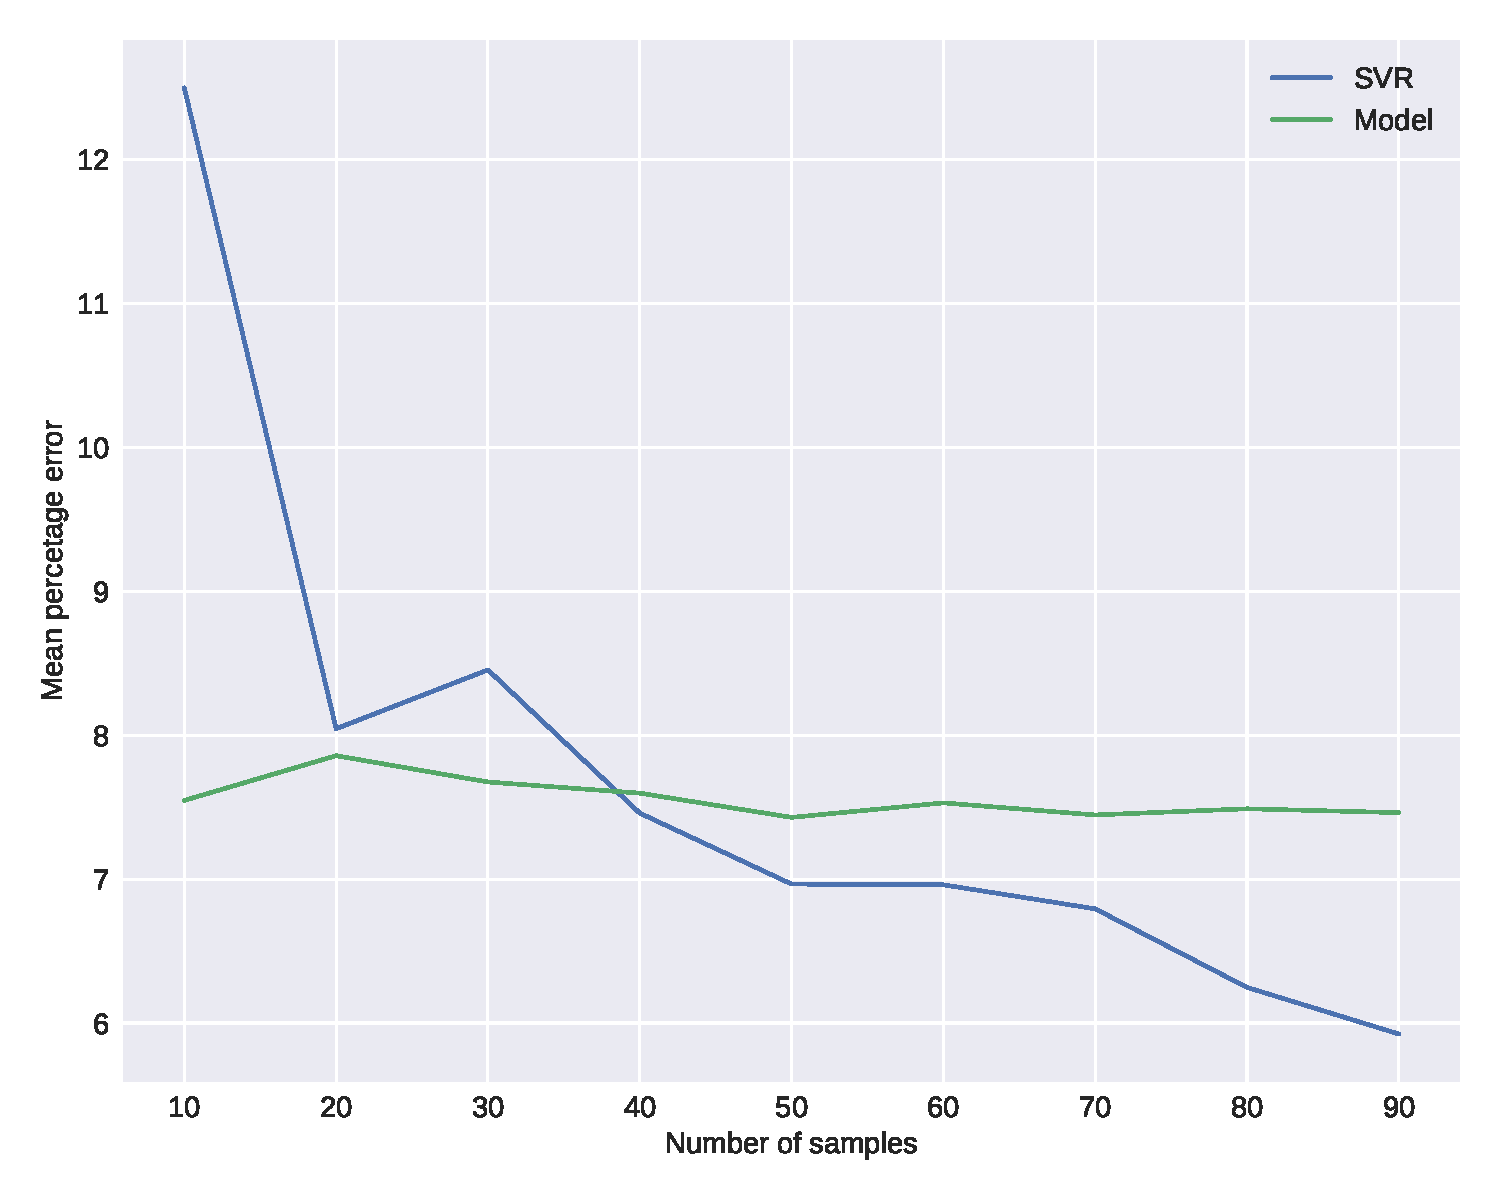
\includegraphics[width=\columnwidth]{models/figures/overhead/completo_ferret_4.pdf}}
		\caption{MPE for Ferret.}
		\label{fig:overhead_ferret}
	\end{subfigure}
	%
	\begin{subfigure}[b]{0.45\textwidth}
		\centerline{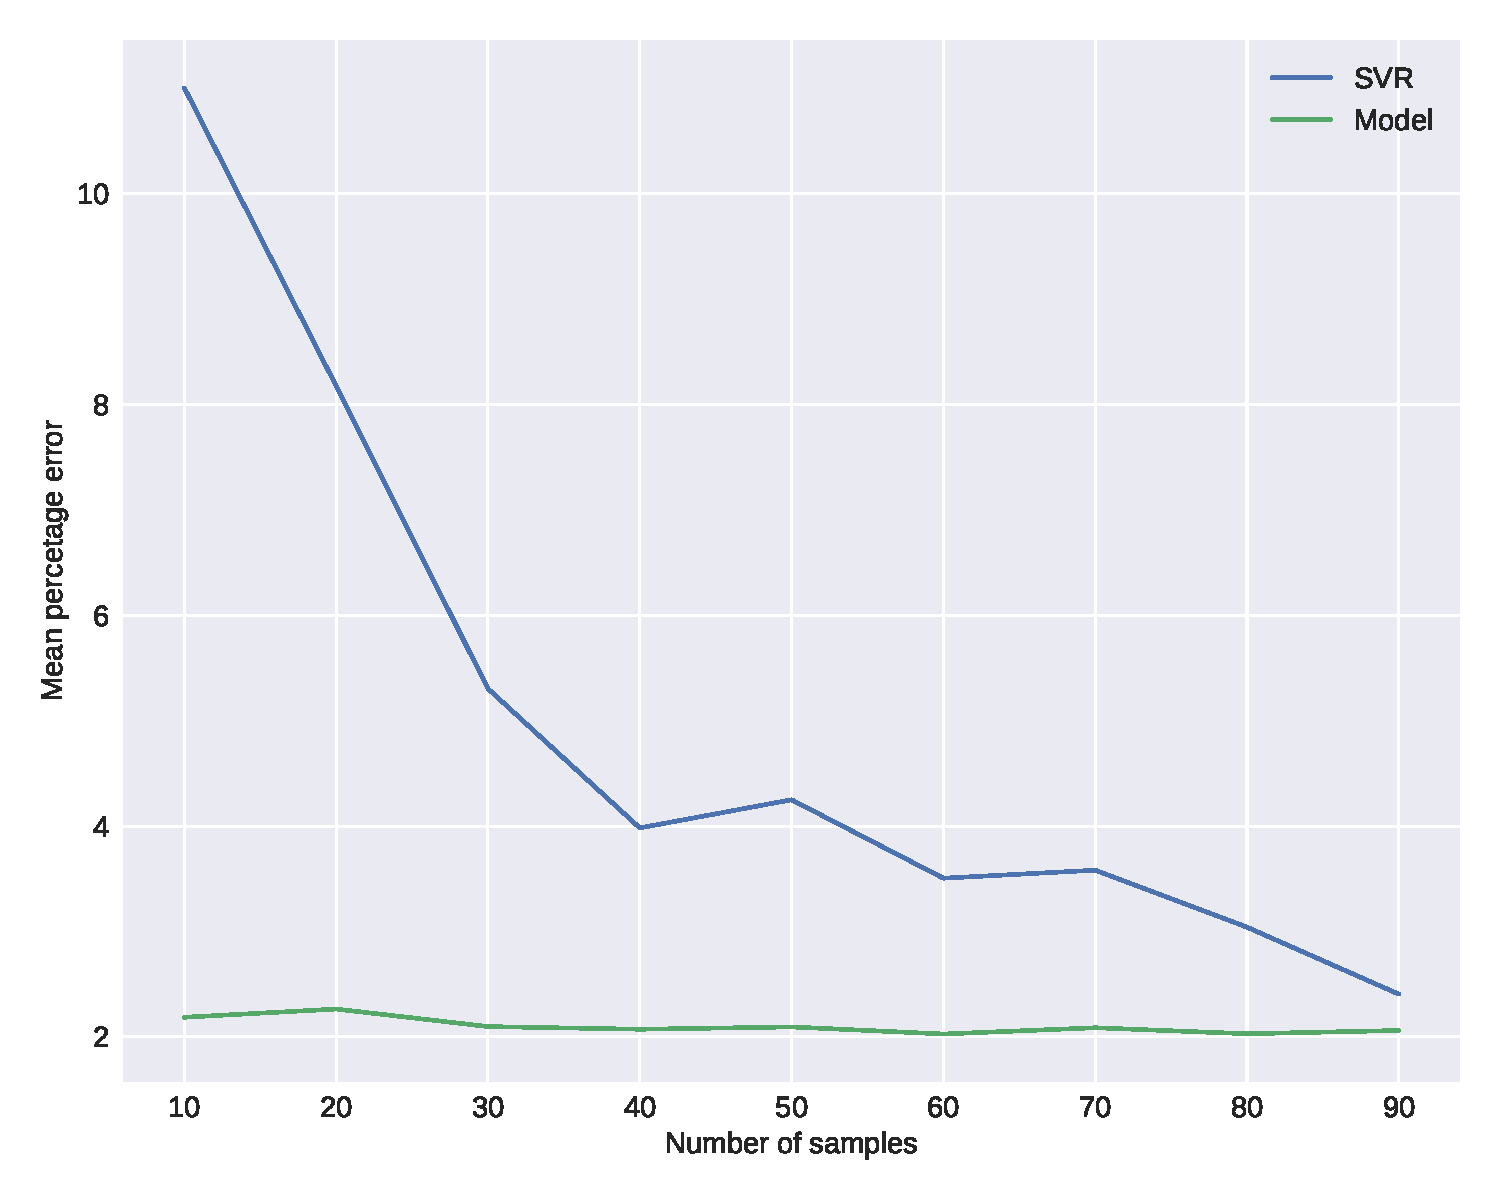
\includegraphics[width=\columnwidth]{models/figures/overhead/completo_black_6.pdf}}
		\caption{MPE for Blackscholes.}
		\label{fig:overhead_black}
	\end{subfigure}
	%
	\par\bigskip
	\begin{subfigure}[b]{0.45\textwidth}
		\centerline{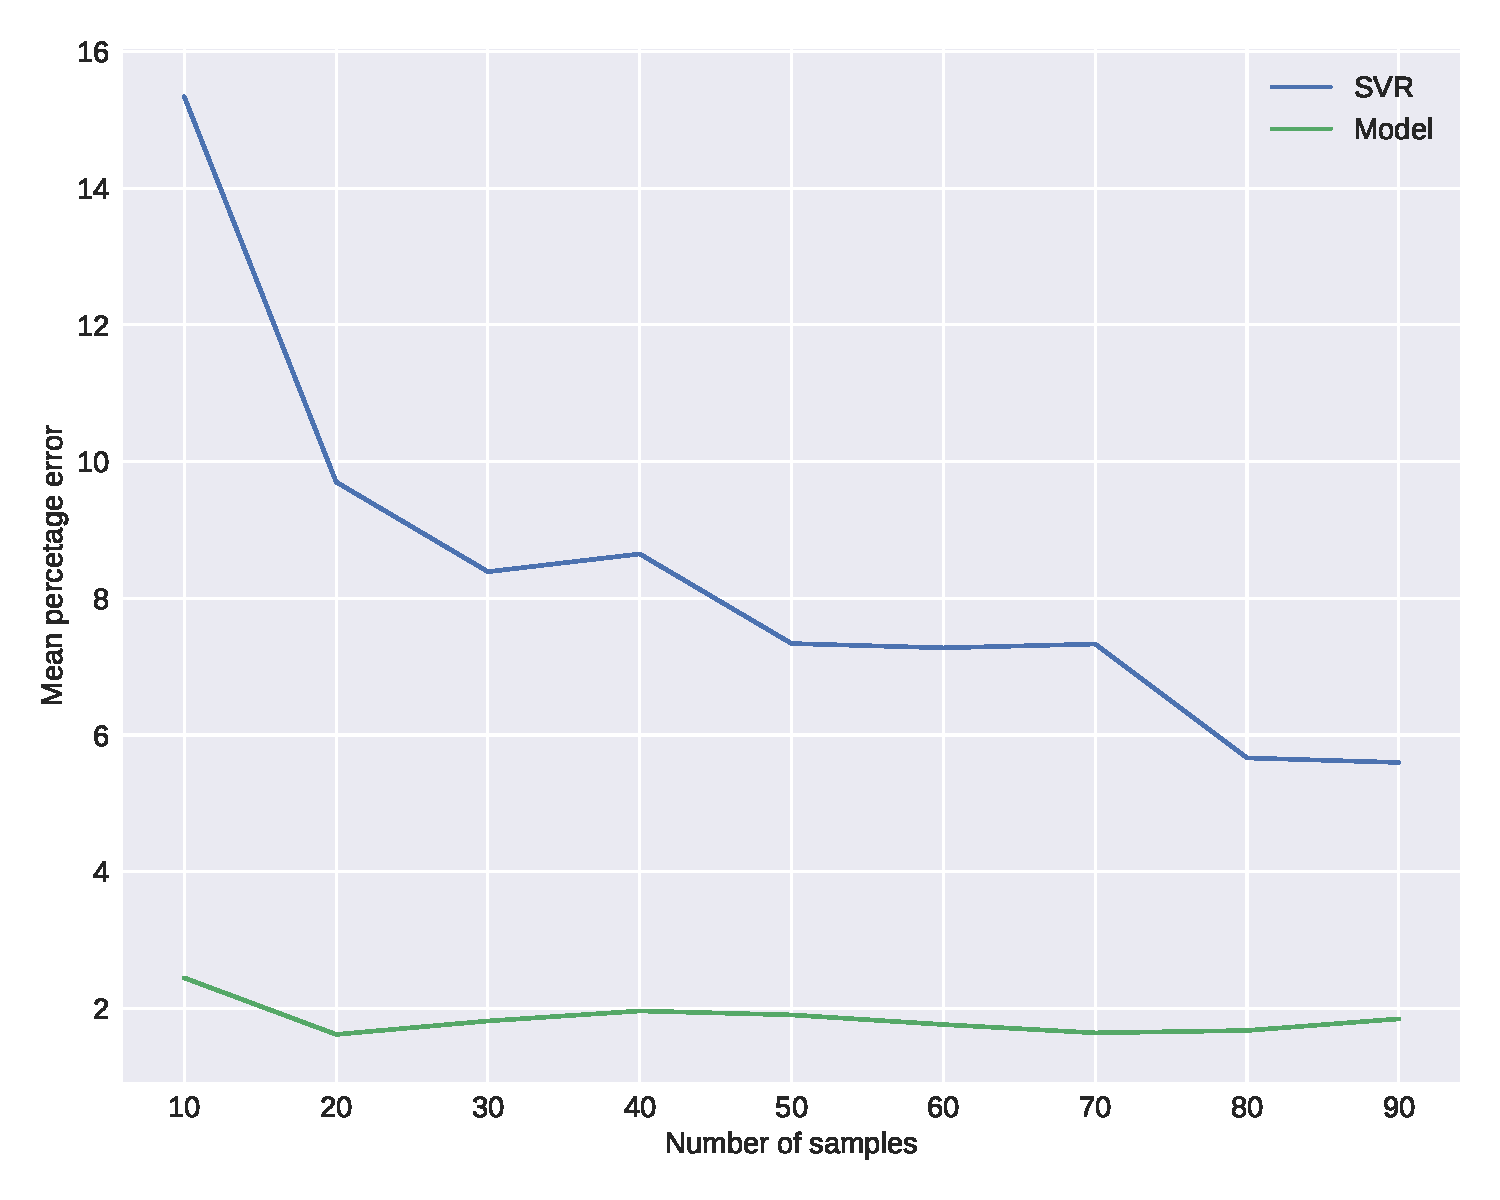
\includegraphics[width=\columnwidth]{models/figures/overhead/completo_x264_4.pdf}}
		\caption{MPE for x264.}
		\label{fig:overhead_x264}
	\end{subfigure}
	%
	\begin{subfigure}[b]{0.45\textwidth}
		\centerline{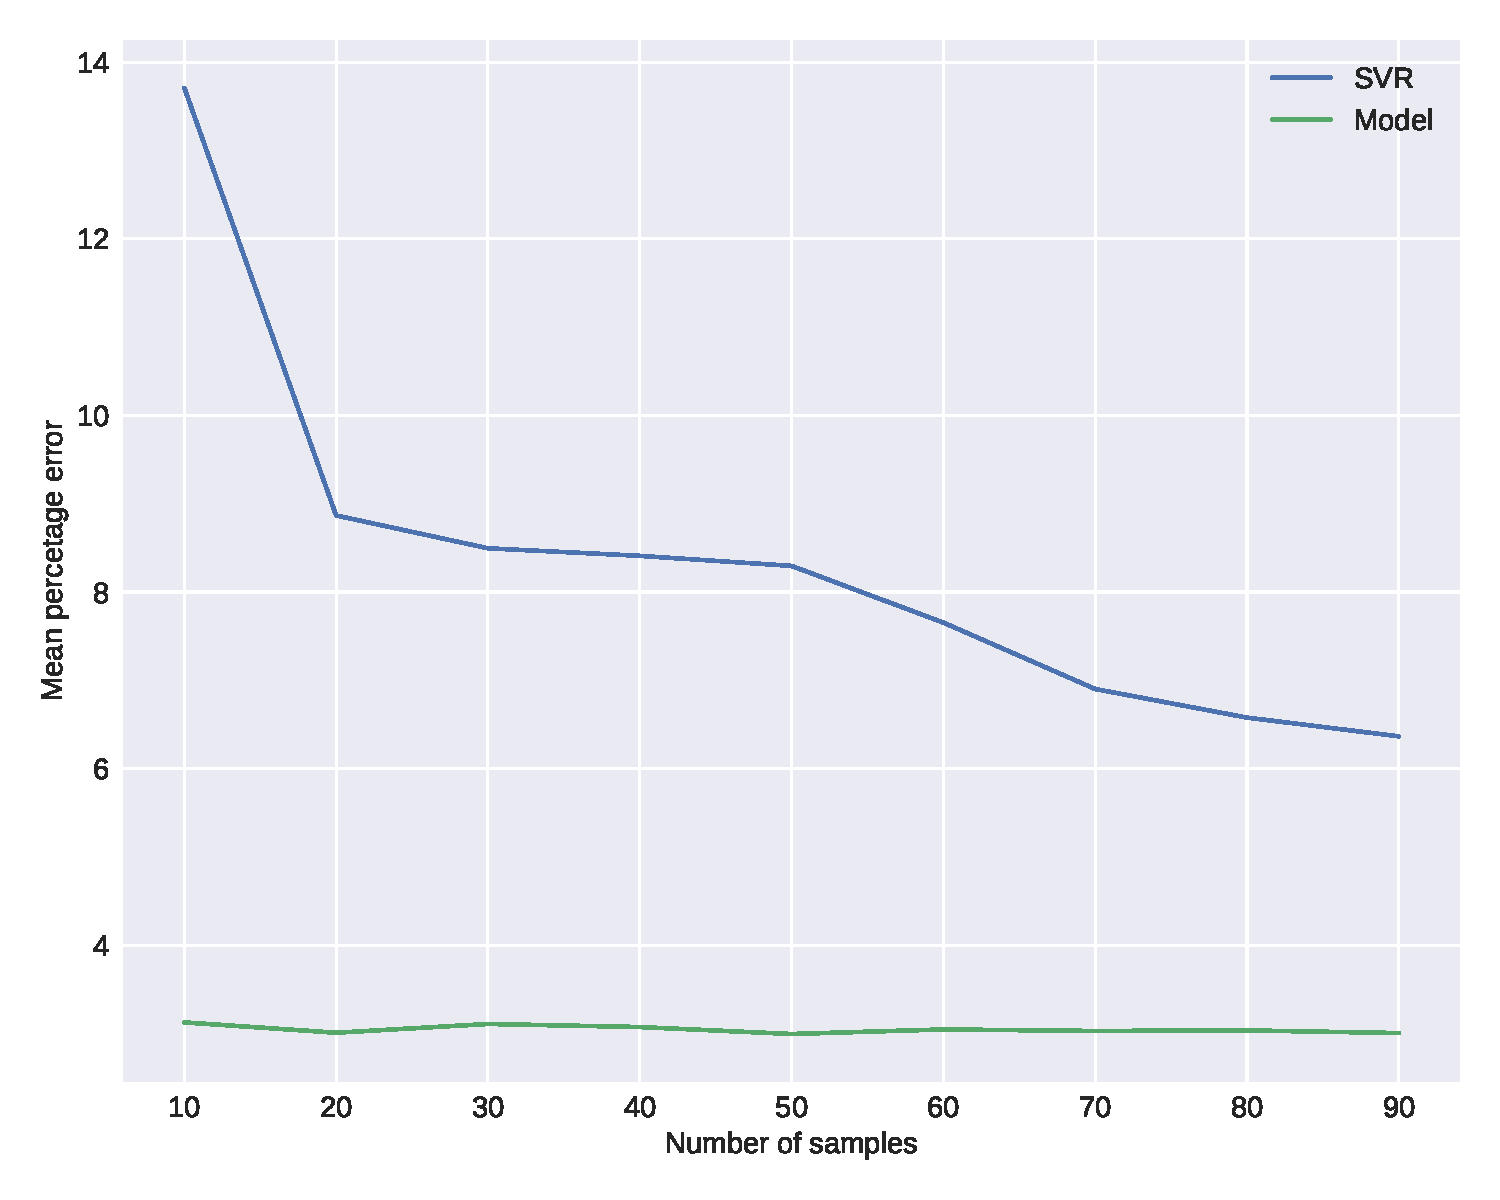
\includegraphics[width=\columnwidth]{models/figures/overhead/completo_dedup_4.pdf}}
		\caption{MPE for Dedup.}
		\label{fig:overhead_dedup}
	\end{subfigure}
	
	\caption{MPE of the case studies versus training size, comparing how many training points is necessary to reach an acceptable result.}
	\label{fig:overheadapps}
\end{figure}

\cref{fig:overheadapps} shows the comparisons of MPE and energy spent to create each model for two selected applications. According to the results, the analytical model is very stable, not changing much as more data is added, while the SVR keeps reshaping to adapt to the data. 
The error of the analytical model is almost constant but that of the SVR, initially very high, drops as more data is used in the training process.
\begin{figure}[H]
	\centering
	\captionsetup[subfigure]{justification=centering}
	\begin{subfigure}[t]{0.45\textwidth}
		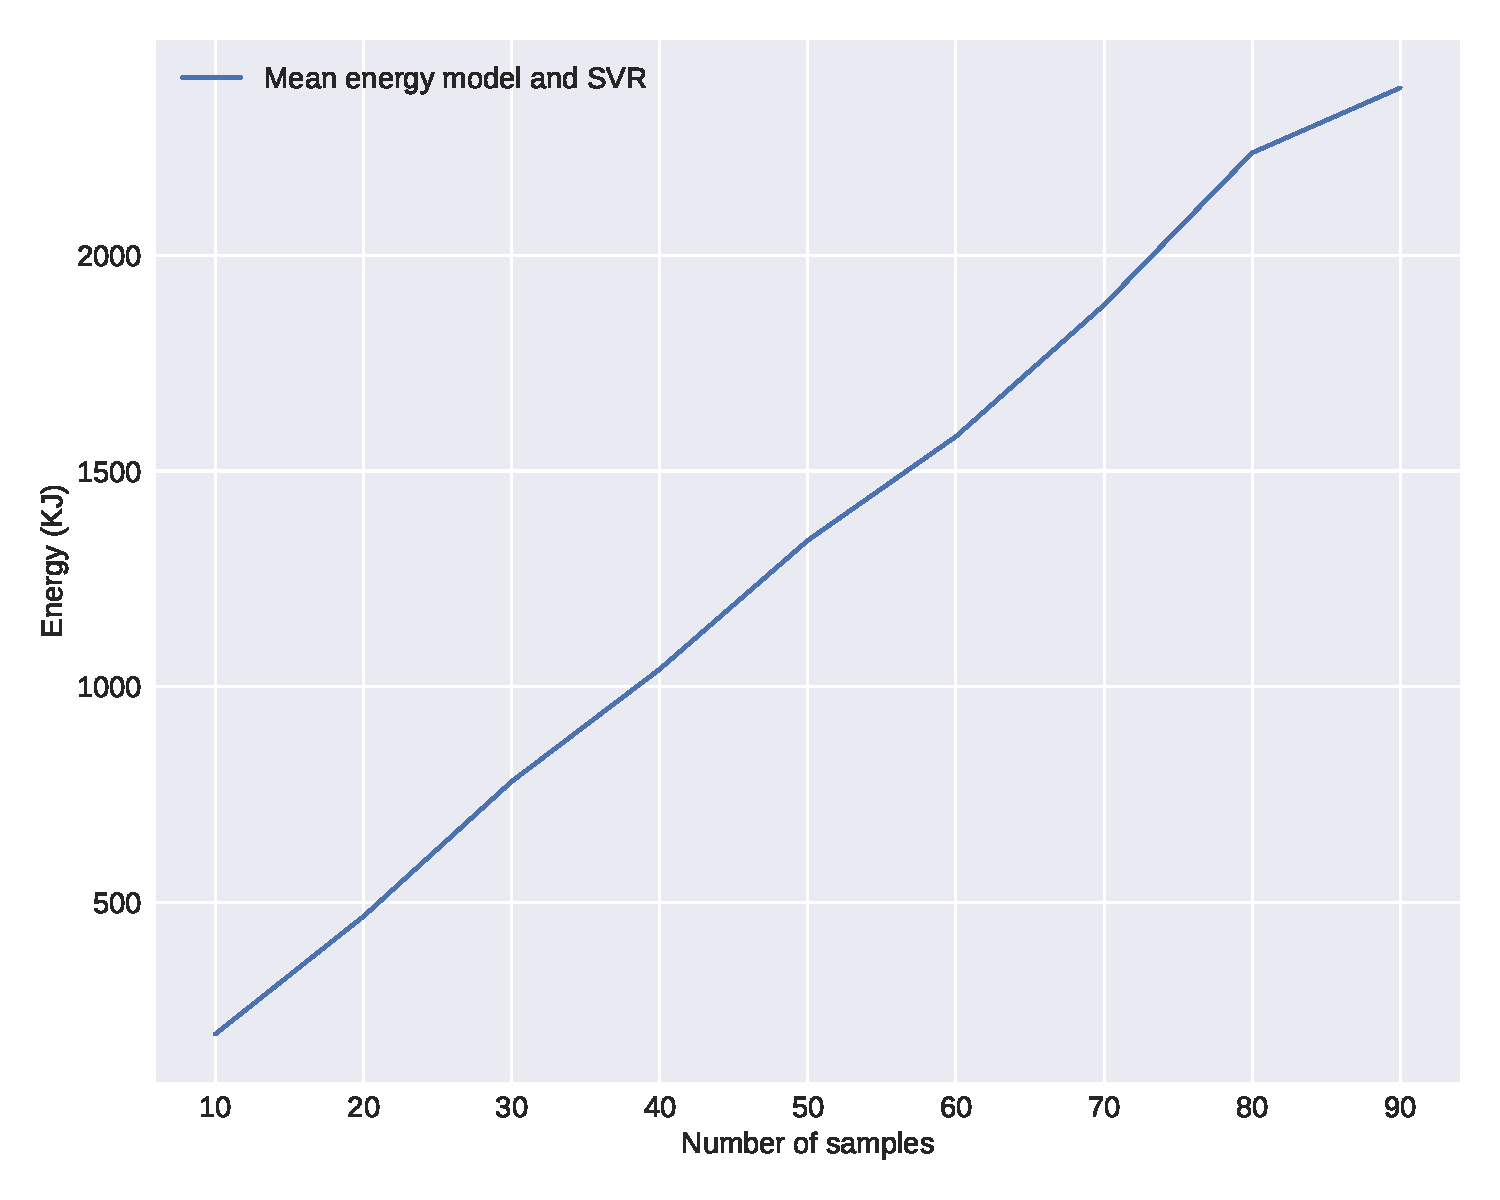
\includegraphics[width=\columnwidth]{models/figures/overhead/overall_energy_10pts.pdf}
		\caption{}
		\label{fig:overall_overhead}
	\end{subfigure}
	%
	%\par\bigskip
	\begin{subfigure}[t]{0.45\textwidth}
		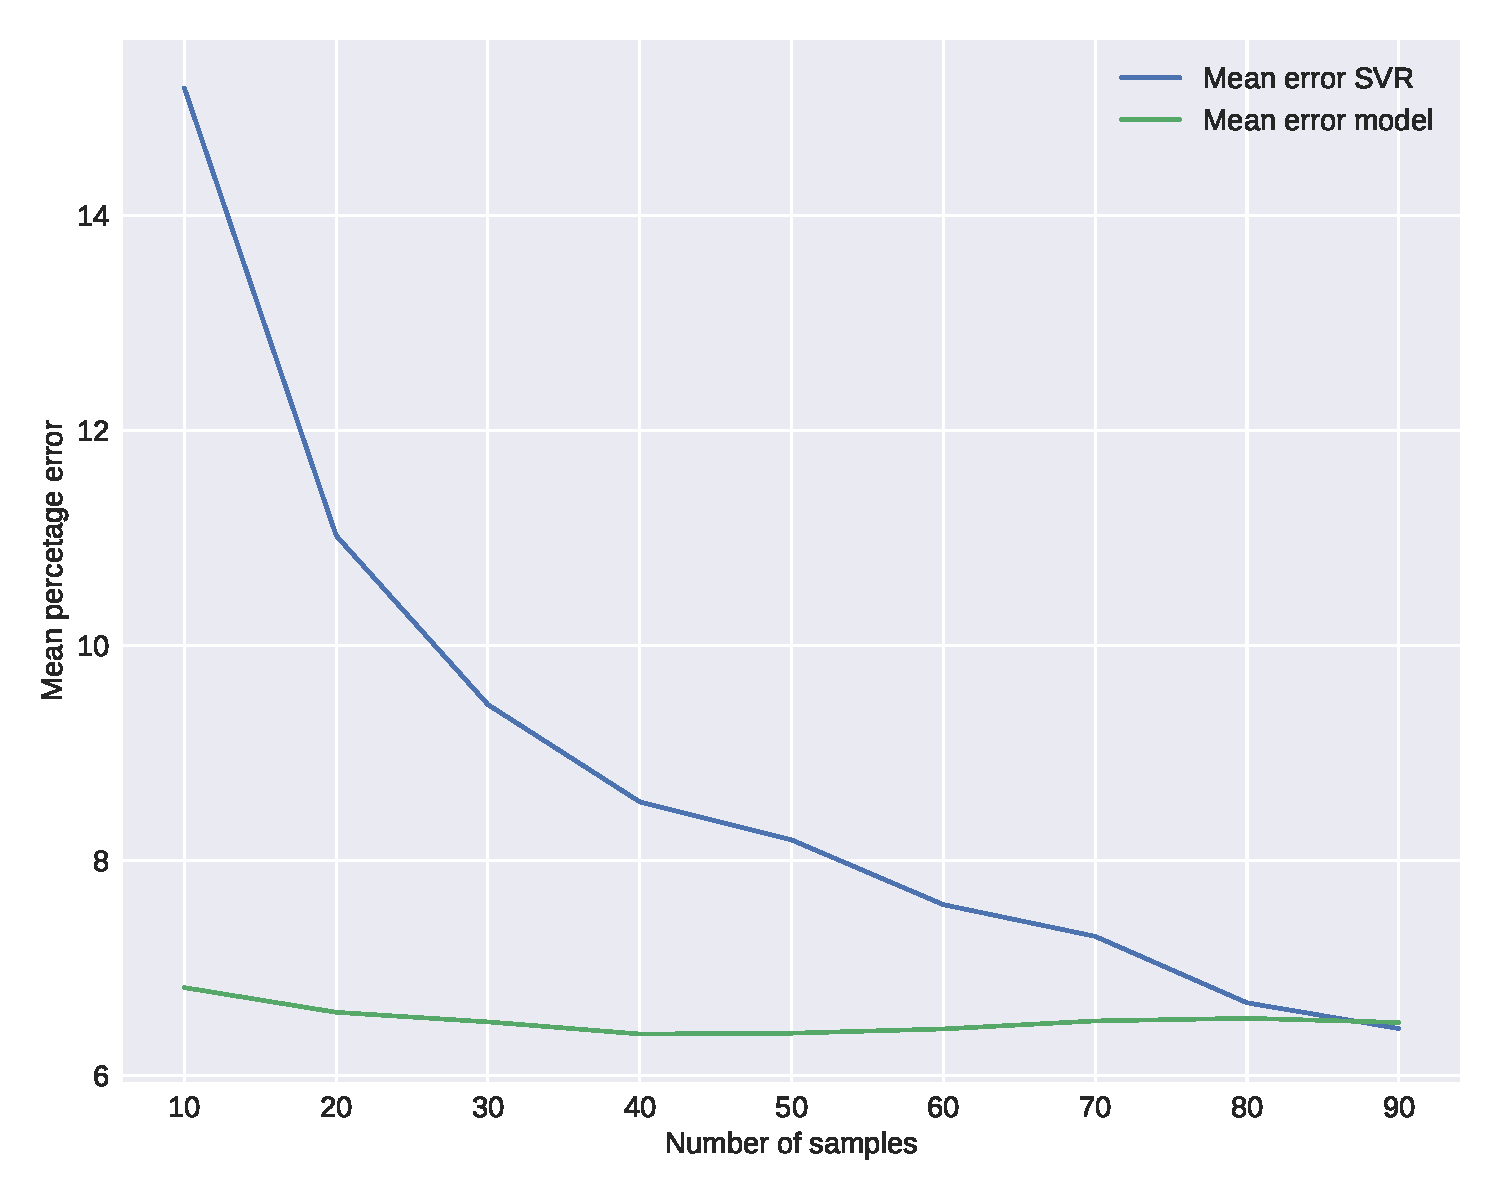
\includegraphics[width=\columnwidth]{models/figures/overhead/overall_mpe_10pts.pdf}
		\caption{
		}
		\label{fig:overall_MPE}
	\end{subfigure}
	\caption{Overall results for energy and MPE for each training size. (\textbf{a}) Average energy spent on all applications during model creation. The two curves are identical because the same data were used to adjust the SVR and the model. (\textbf{b}) MPE of all applications: SVR needs 10 times more data to have an MPE lower than the proposed model.}
	\label{fig:overall_train}
\end{figure}

\cref{fig:overall_train} presents the overall results, with the mean energy overhead and MPE for all applications.
The meeting point of the MPE for the SVR and the proposed model can be extracted from \cref{fig:overall_train}b.
It shows that, in around 90 configurations, the SVR starts to have a smaller error. The cost of that is the linear increase in energy spent on training. The increase in energy, about 10 times more, can be observed in \cref{fig:overall_train}a.

\section{Analysis} \label{sec:analysis}
One of the most significant advantages of using an analytical model is the understanding of the problem that an equation provides, making many different kinds of analysis possible that are otherwise impossible with a machine learning model. In this section, we discuss one of the possible analyses. In the following figures, we try to understand the contribution of each parameter of the equation to the total energy consumption.

For this analysis, we took the model of one of the applications and, varying one parameter of the equation, we display the energy versus performance (time) for all configurations. After that, we computed the Pareto frontier, a set of all Pareto efficient allocations, i.e., all the configurations where resources cannot be reallocated to make one individual better off without making at least one individual worse off. This gives us all the configurations where we have an optimal trade-off of performance and energy to choose from.


\cref{fig:pareto_static} shows the Pareto frontier for several values for the static power parameter ($c_3$ in \cref{eq:en_final}) with configurations of frequency ranging from 1.2 to 5 GHz and cores from 1 to 64, so that we can also have an idea of what is the tendency when we increase the frequency and number of cores.

\begin{figure}[H]
	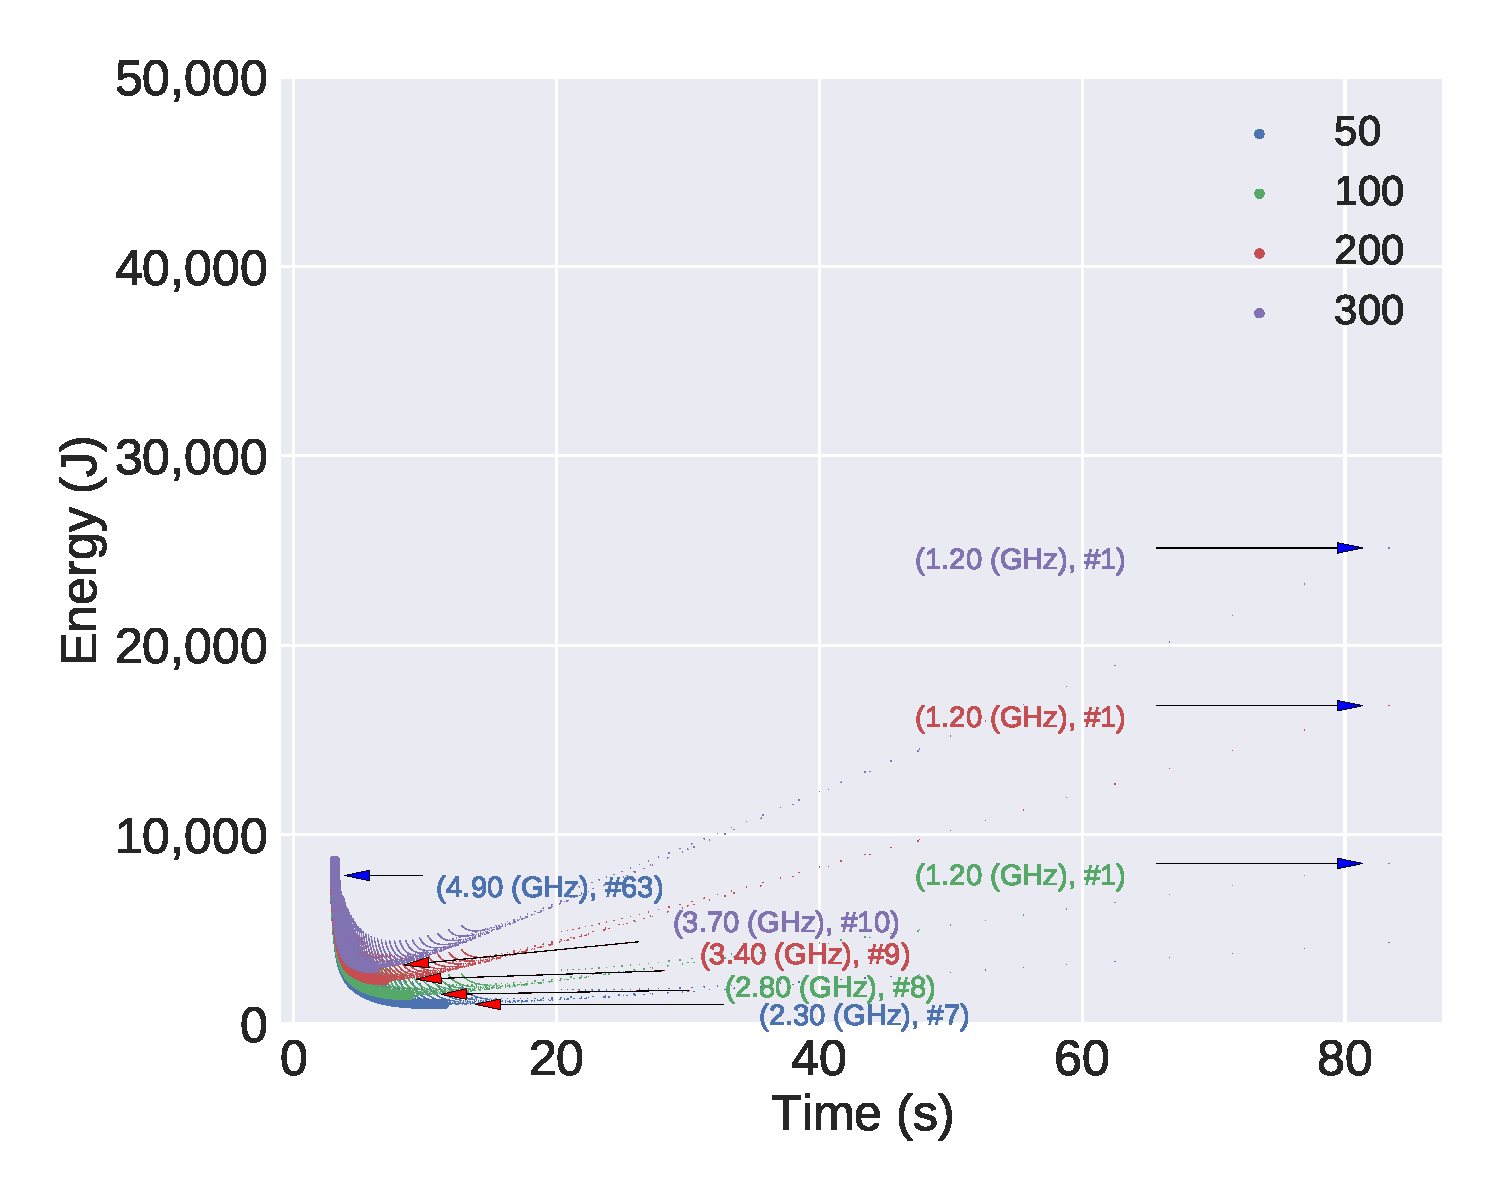
\includegraphics[width=\columnwidth]{models/figures/analisys/pareto_static_high.pdf}
	\caption{Pareto frontier for several values of static power parameter. The arrows with blue heads indicate the maximum energy, while the arrows with a red head the minimal energy for each corresponding curve.}% In four-digit numbers, no comma or spaces to indicate thousand, whatever the numbers are in the table or body text, e.g., 4500; More than five-digit numbers, should have comma, e.g. 59,400; 899,302. Please revise the figure.
	\label{fig:pareto_static}
\end{figure}
%Fixed

From this figure, we can see that when increasing the value of the static power parameter, the total energy consumption increases as expected. We can also observe that the values that minimize the total energy consumption tend to be high frequency and multiple cores. This is one of the consequences of increasing the static power factor. As the dynamic factor proportionally decreases, its variables tend to have less impact on total consumption, enabling configurations with high frequency and several cores. This also enables chip-level optimization for choosing components that change the ratio between static and dynamic power.


\cref{fig:pareto_w} shows the Pareto frontier in the same ranges described before but for the parameter corresponding to the level of parallelism of the application ($w$ in  \cref{eq:en_final}).

\begin{figure}[H]
	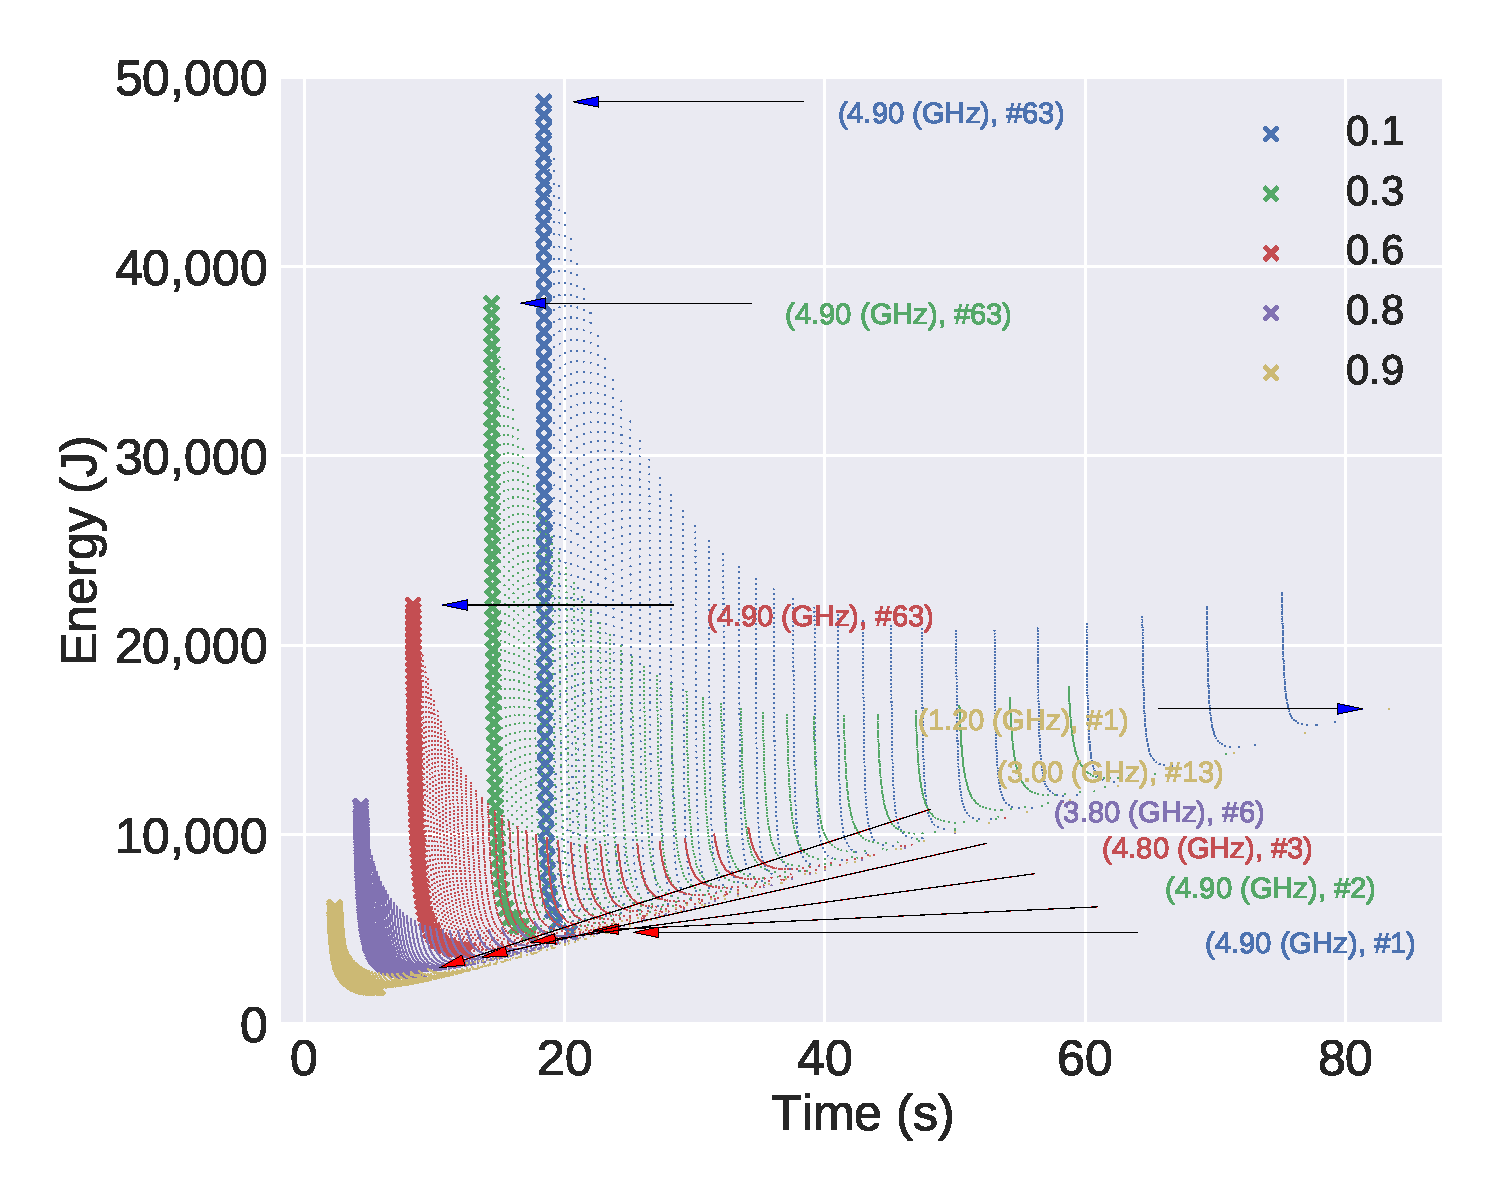
\includegraphics[width=\columnwidth]{models/figures/analisys/pareto_w_high.pdf}
	\caption{Pareto frontier for several values of static power parameter. The arrows with blue heads indicate the maximum energy, while the arrows with a red head, the minimal, for each corresponding curve.}% In four-digit numbers, no comma or spaces to indicate thousand, whatever the numbers are in the table or body text, e.g., 4500; More than five-digit numbers, should have comma, e.g. 59,400; 899,302. Please revise the figure.
	\label{fig:pareto_w}
\end{figure}
%Fixed

In  \cref{fig:pareto_w}, we observe that, as the parallelism level increases the total energy decreases. The number of cores tends to be higher with a higher level of parallelism as expected, and the frequency shows an inverse relation.


\section{DVFS and DPM Optimization} \label{sec:dvfs_dpm_optminzation}
The effectiveness of the proposed approach during optimization was evaluated with a simple algorithm that finds the optimal frequency and number of active cores from the proposed equation. The results were then compared to the Linux default choices for power management.

With \cref{eq:en_final}, it is possible to calculate energy consumption estimates for each possible configuration since there is a finite range of possible values for the frequency and number of cores. It is also possible to apply constraints on the execution time, frequency, and the number of active cores. Then, the configuration that minimizes energy consumption for a given input can be selected. The complete workflow is shown in \cref{fig:optim_workflow}. We can see that any optimization problem can be structured with our model and the system's constraints. In the following examples, the optimization problem that we build is to minimize the energy equation given the constraints of possible frequencies and the number of cores that our system can run. The algorithm selected to minimize was the newton-CG~\cite{Royer2020AOptimization}.

Current HPC managers leave to the user the choice of how many cores to use. On this basis, three situations were analyzed in relation to the number of cores:

\begin{enumerate}
	\item Worst choice: number of cores that maximize the total energy consumed;
	\item Random choice: energy consumed for a random choice of the number of cores;
	\item Best choice: number of cores that minimize the total energy consumed (oracle).
\end{enumerate}
\begin{figure}[H]
	\centering
	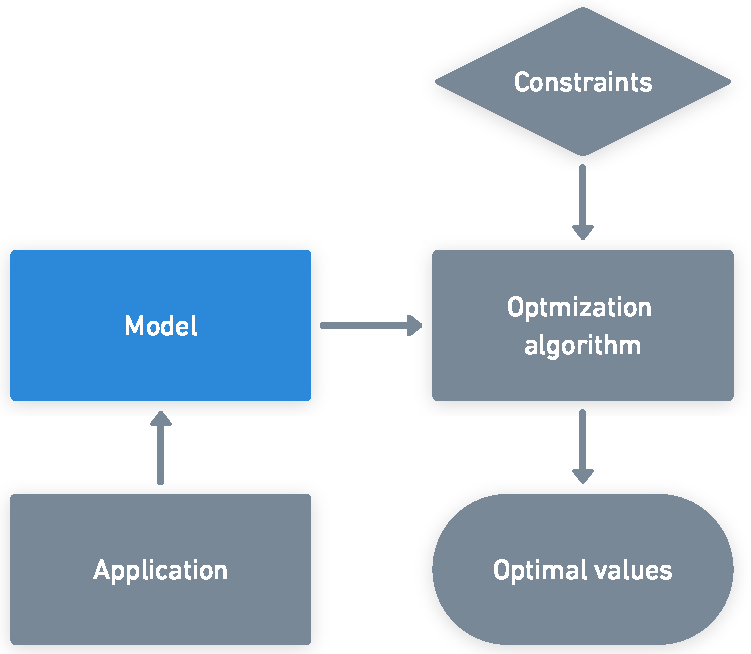
\includegraphics[width=0.8\columnwidth]{models/figures/DVFS optim.pdf}
	\caption{Optimization workflow showing how DVFS and DPM optimization could be implemented from ou model.}
	\label{fig:optim_workflow}
\end{figure}


The default option for the Linux governor is Ondemand, and, by default, it has no DPM control for the number of active cores. As Ondemand only performs DVFS, \textls[-15]{for comparison, each application was executed with all available cores in the system, from 1 to 32.}

\textls[-15]{Figures \ref{fig:energy_worst_case}--\ref{fig:energy_best_case}, show the energy savings with respect to Ondemand, i.e., $\frac{Ondemand-Model_{min}}{Ondemand}$} for the three cases described above. The savings and losses for each case are:

\begin{enumerate}
	\item Worst choice: save 69.88\% on average;
	\item Random choice: save 12.04\% on average;
	\item Best choice: lost 14.06\% on average.
\end{enumerate}

\begin{figure}[H]
	\centering
	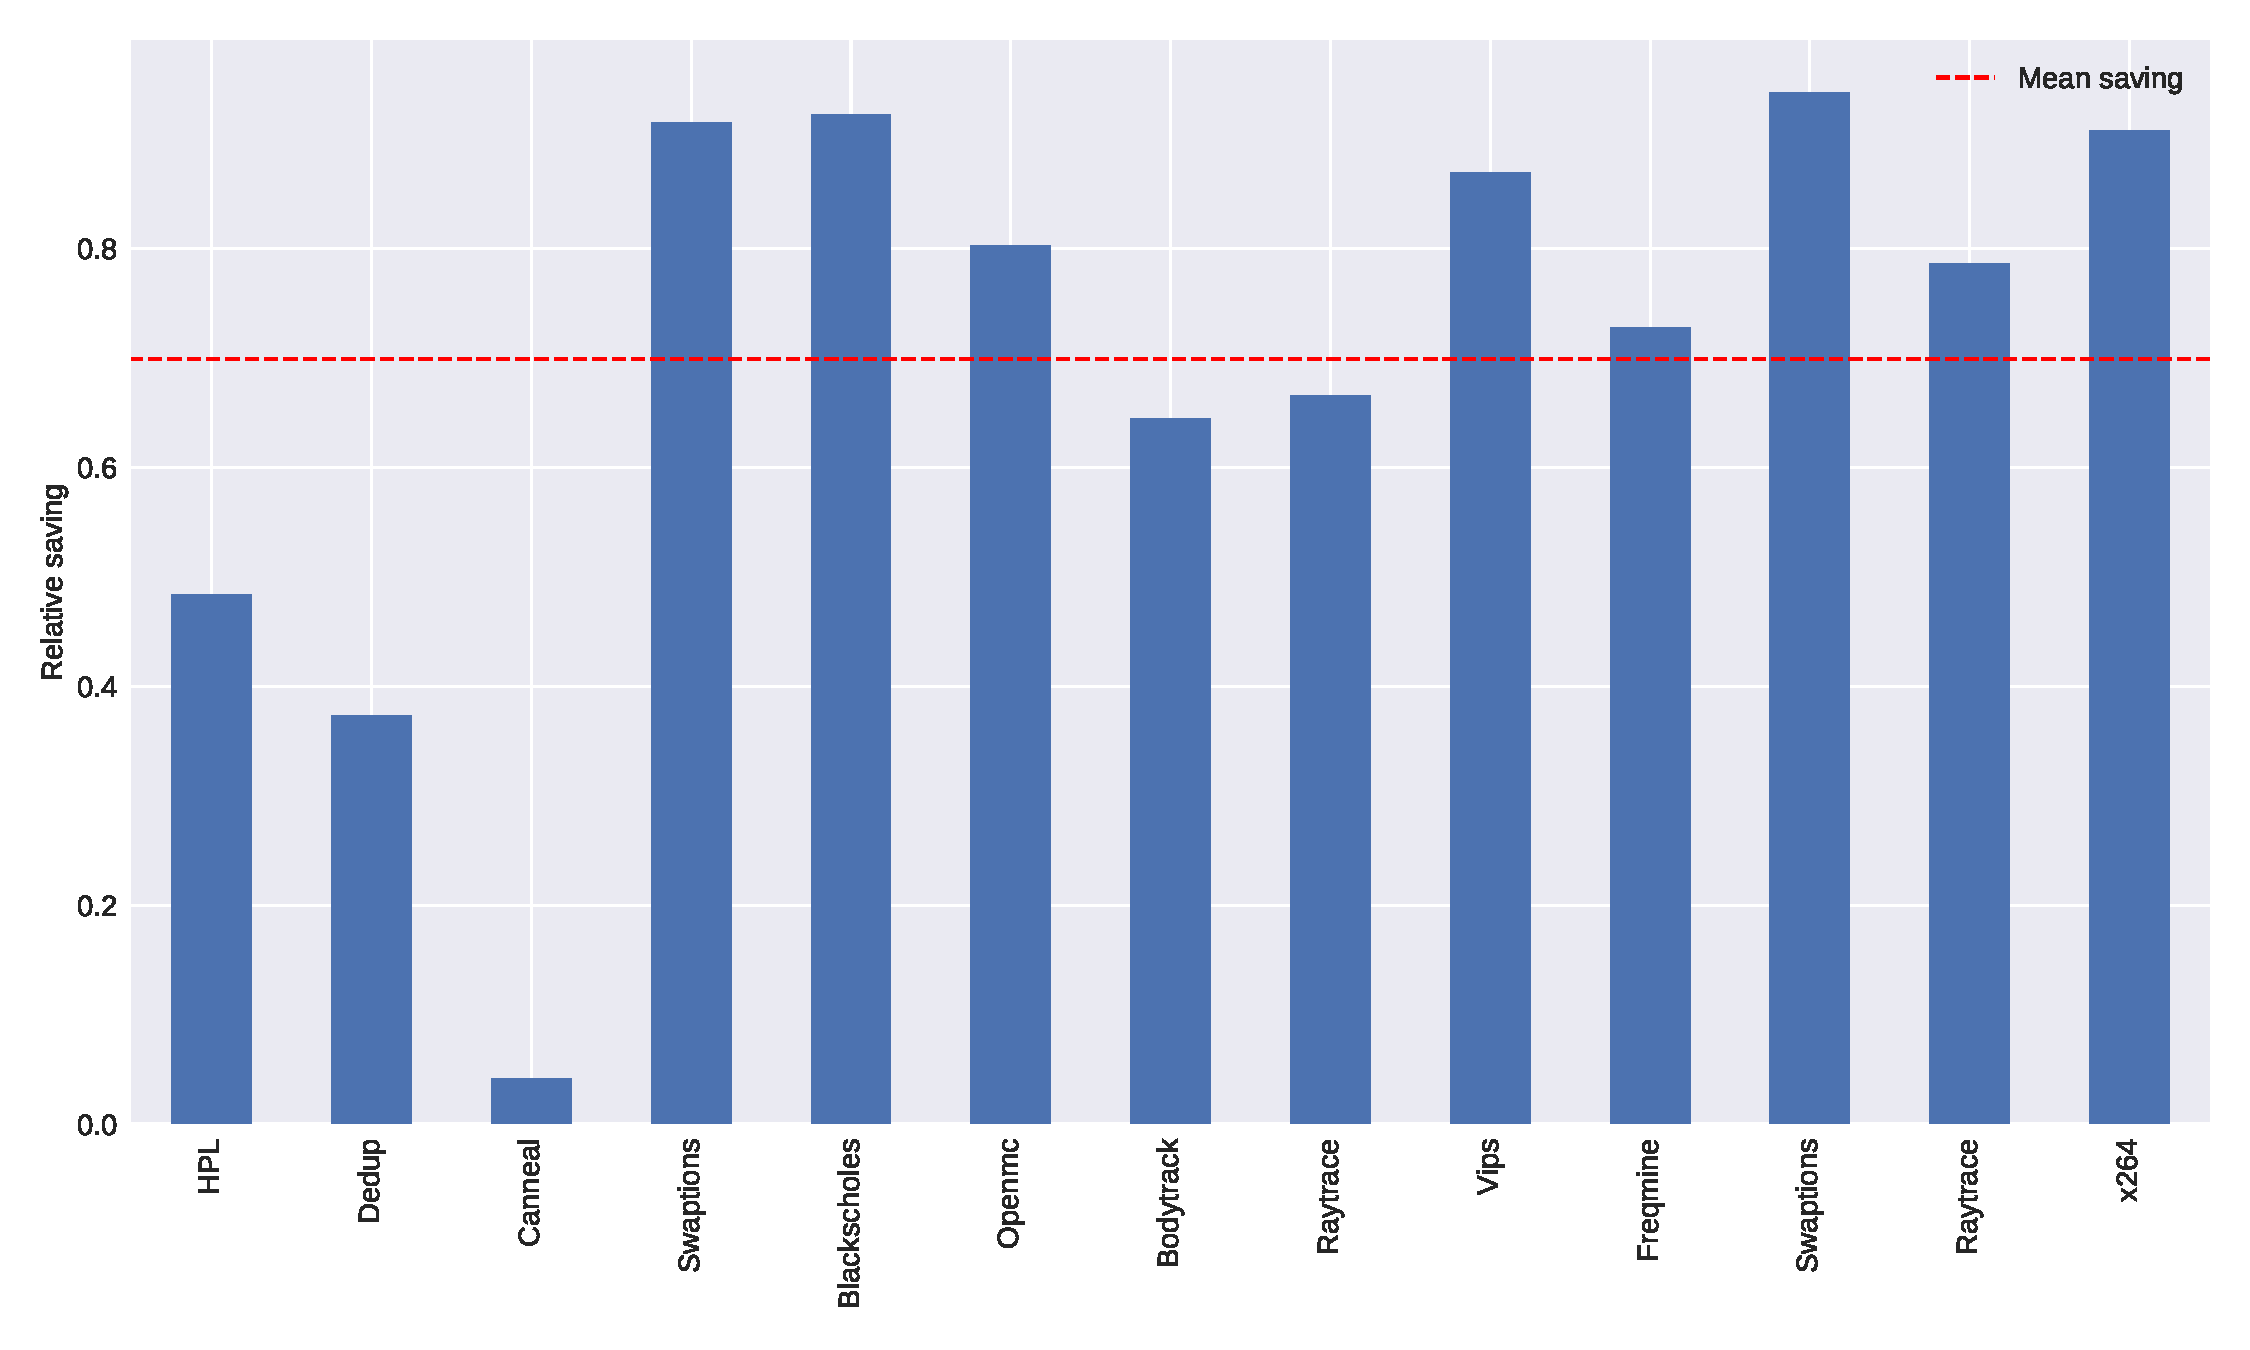
\includegraphics[width=\columnwidth]{models/figures/dvfs_cmp_max.pdf}
	\caption{Energy savings comparisons between the proposed model and the Worst case.}
	\label{fig:energy_worst_case}
\end{figure}

\begin{figure}[H]
	\centering
	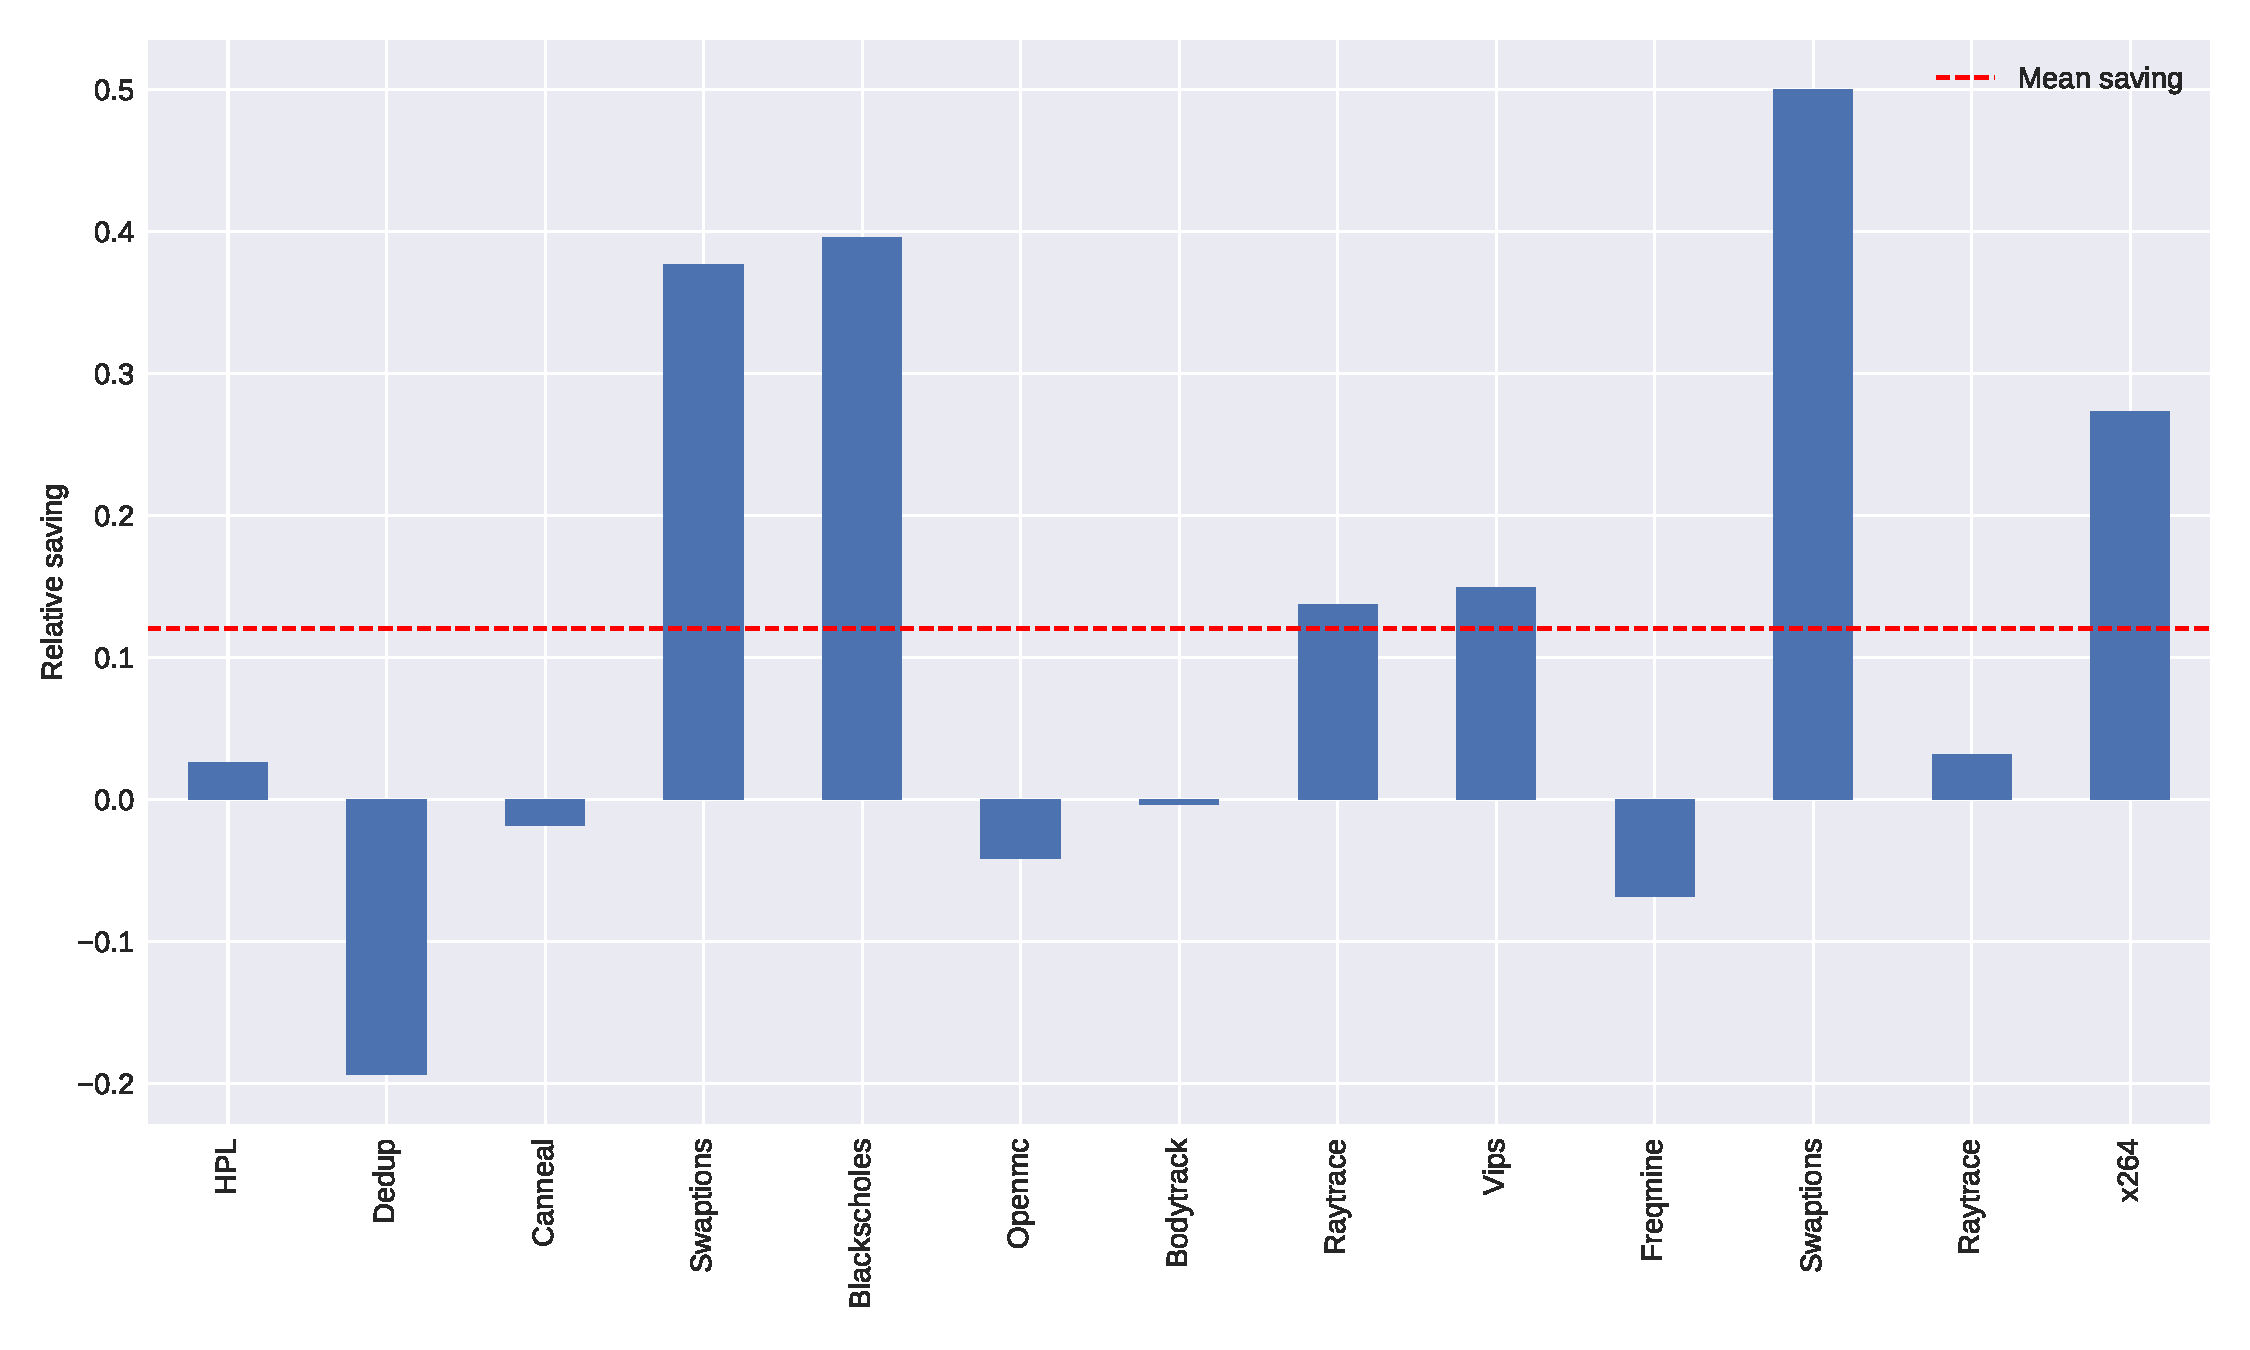
\includegraphics[width=\columnwidth]{models/figures/dvfs_cmp_mean.pdf}
	\caption{Energy savings comparisons between the proposed model and the Random case.}
	\label{fig:energy_mean_case}
\end{figure}

By default, operating systems do not implement DPM at the core level, and, in HPC, the user usually explicitly chooses the number of cores to run their job. To give a better idea of the impact on the energy consumption of DPM at the core level, we analyzed the choices of the number of cores over a period of one year in the HPC center at UFRN. The result is plotted in~\cref{fig:cpu_requests}.


It is of note that the most common choice of many regular users is a single core requested per job, matching the worst-case choice for all applications analyzed in this investigation. The best choice was quite often 32 cores, which is the third most popular choice among users, but it is 72 times less frequent than 1 core. This led us to envision how much energy could be saved and encouraged us towards future research using the proposed model for DPM or more advanced optimization algorithms.

In practice, this approach can be implemented by allowing the resource manager to perform these changes for the user using pre-scripts and post-scripts for high energy consumption job submissions.
\begin{figure}[H]
	\centering
	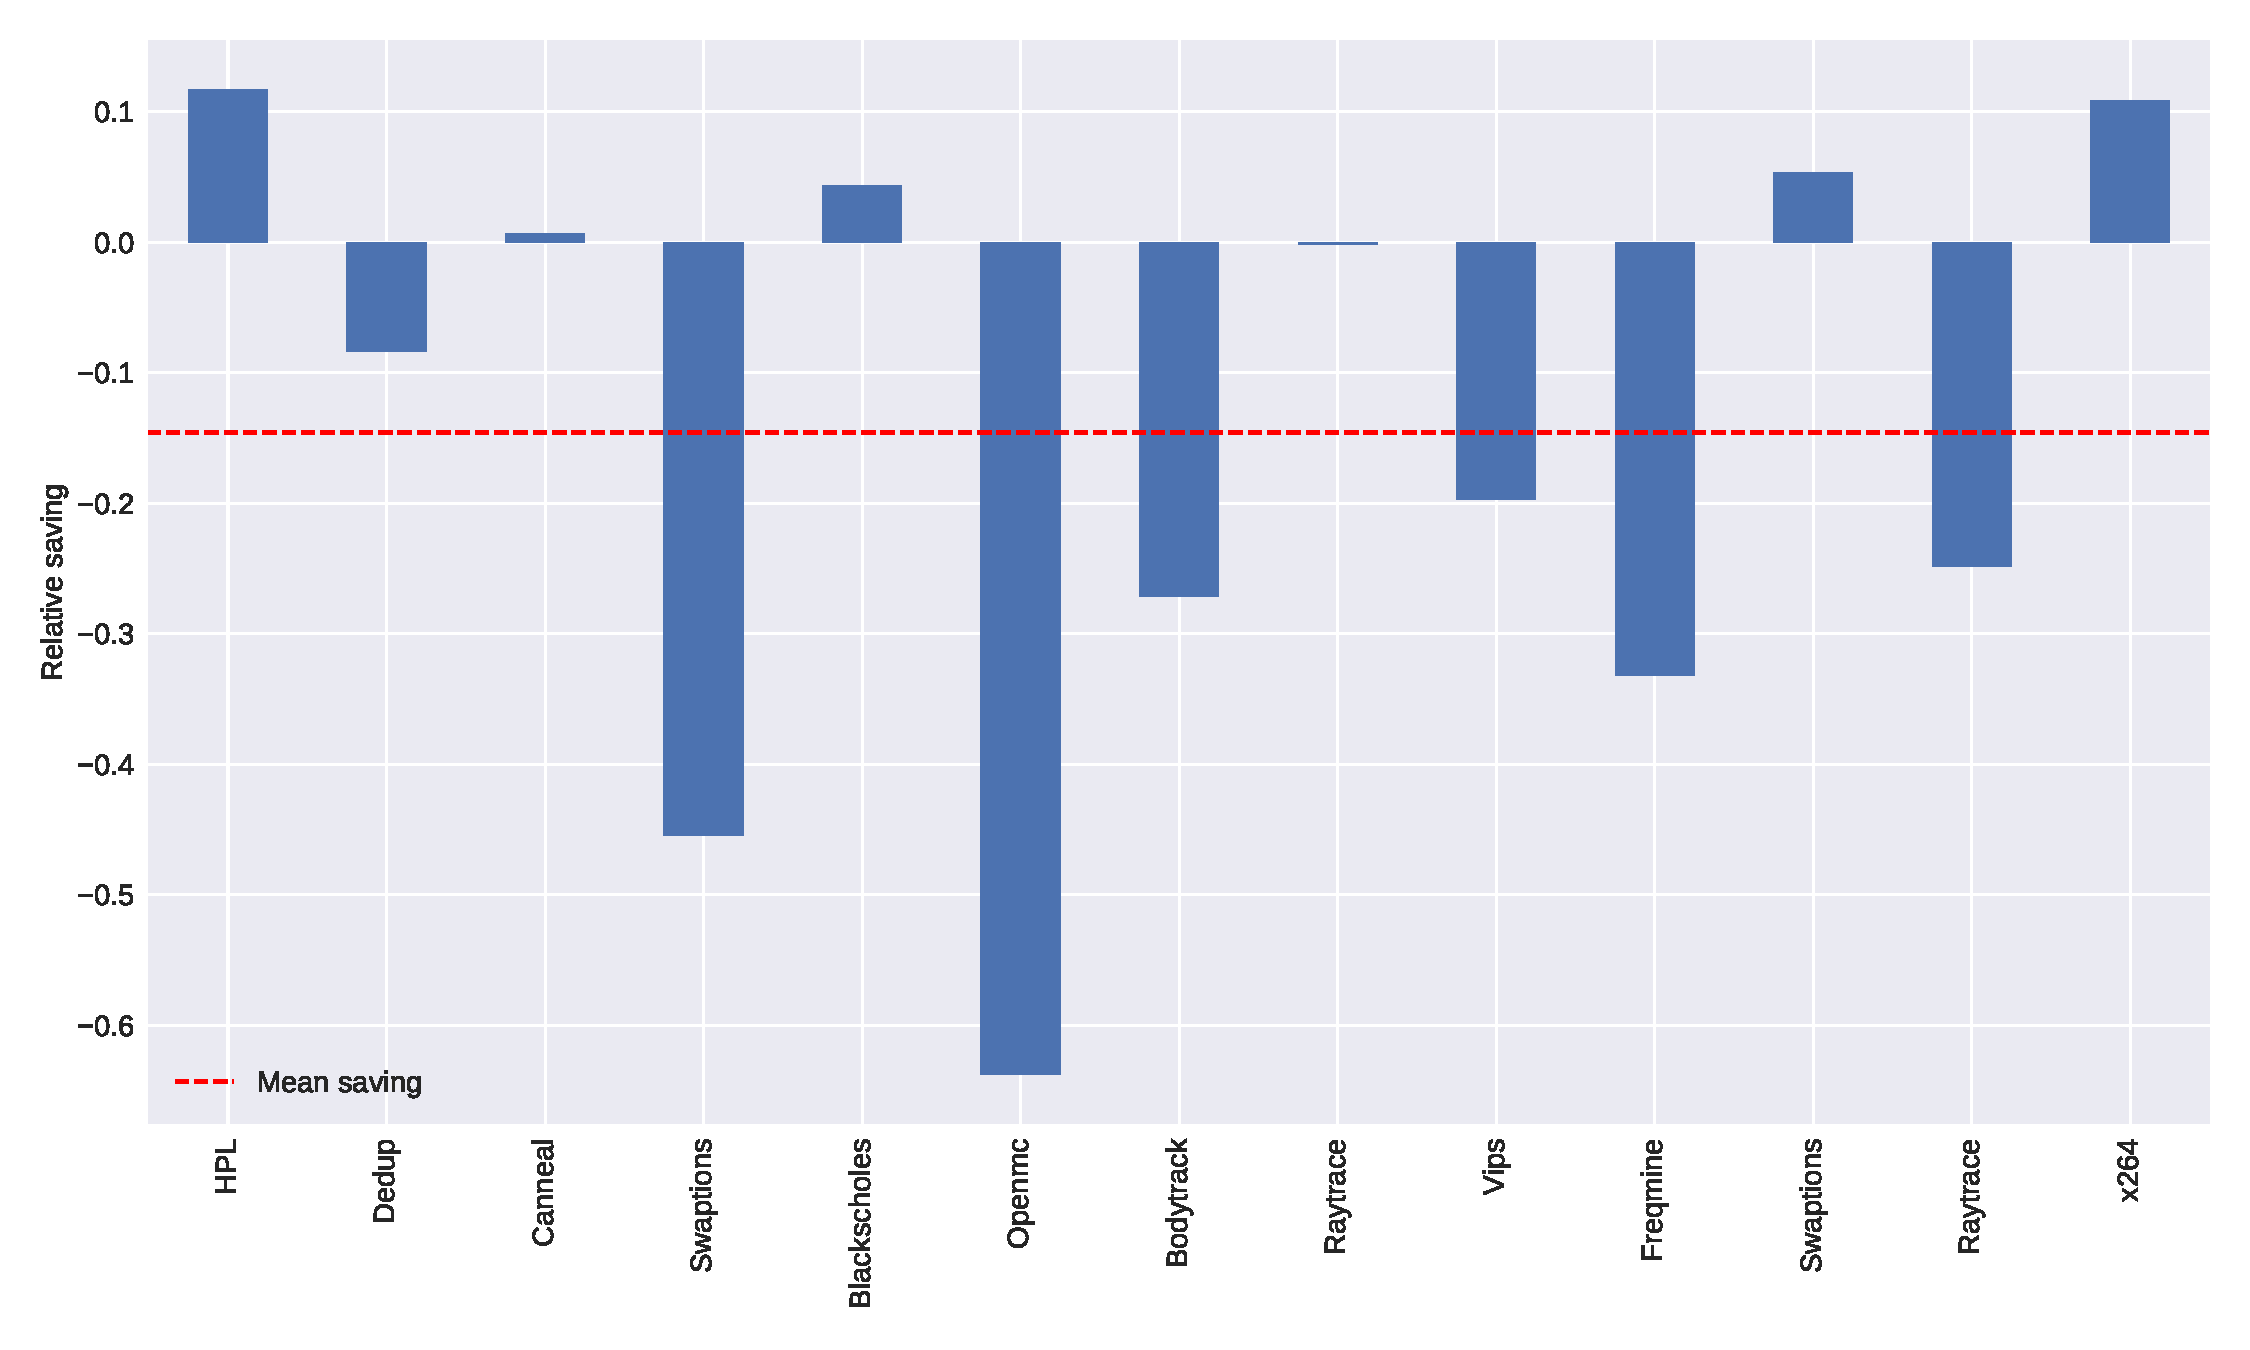
\includegraphics[width=\columnwidth]{models/figures/dvfs_cmp_32.pdf}
	\caption{Energy savings comparisons between the proposed model and the Best case.}
	\label{fig:energy_best_case}
\end{figure}
\vspace{-12pt}

\begin{figure}[H]
	\centering
	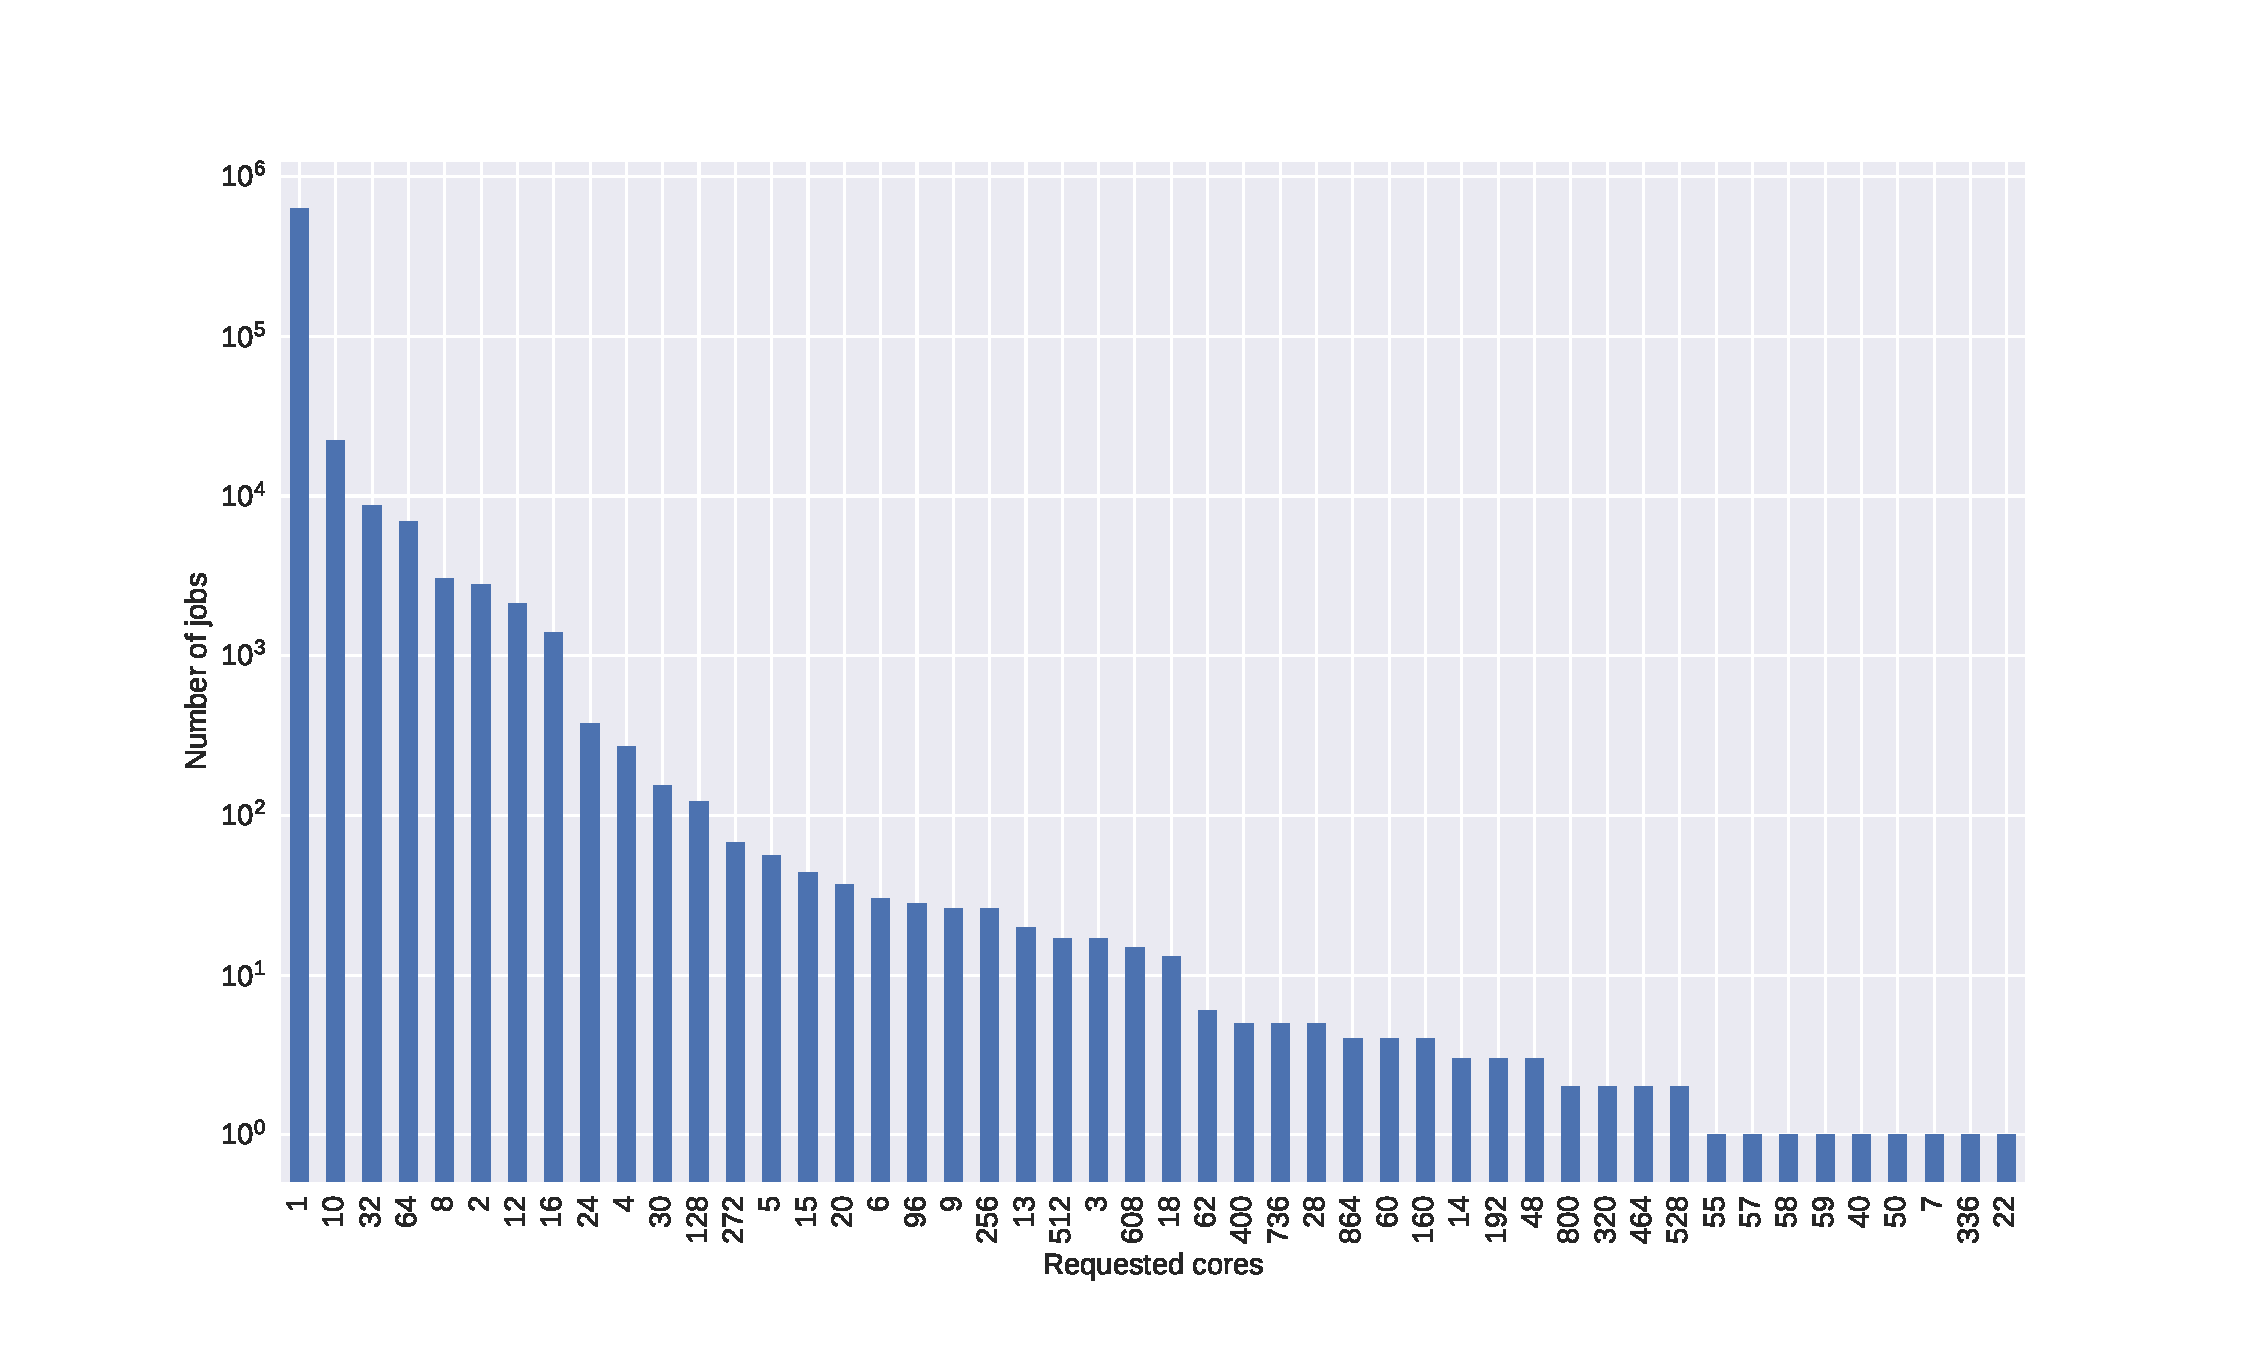
\includegraphics[width=\columnwidth]{experiments/figures/cpu_requestes.pdf}
	\caption{Number of CPU requests during one year in HPC cluster, sorted by the number of cores requested per job.}
	\label{fig:cpu_requests}
\end{figure}

%\section{PMCs}
%
%\section{Energy per instruction}
%
%\begin{lstlisting}
%xor rcx, rcx
%mov rax, 1
%mov rdx, 0
%
%loop:
%	targ_inst(*arg)
%	targ_inst(*arg)
%	targ_inst(*arg)
%	targ_inst(*arg)
%	targ_inst(*arg)
%	targ_inst(*arg)
%	targ_inst(*arg)
%	targ_inst(*arg)
%	targ_inst(*arg)
%
%add rcx, 1
%cmp rcx, 9999999
%jne loop
%\end{lstlisting}
%
%Estimating the energy of the instruction from this benchmark
%
%$E_{total}=9999999(\frac{10}{13}inst+\frac{3}{13}loop)$
%
%$E_{total}=7692306*inst+constant$
%
%\subsection{Generic}
%
%\begin{figure}
%	\centering
%	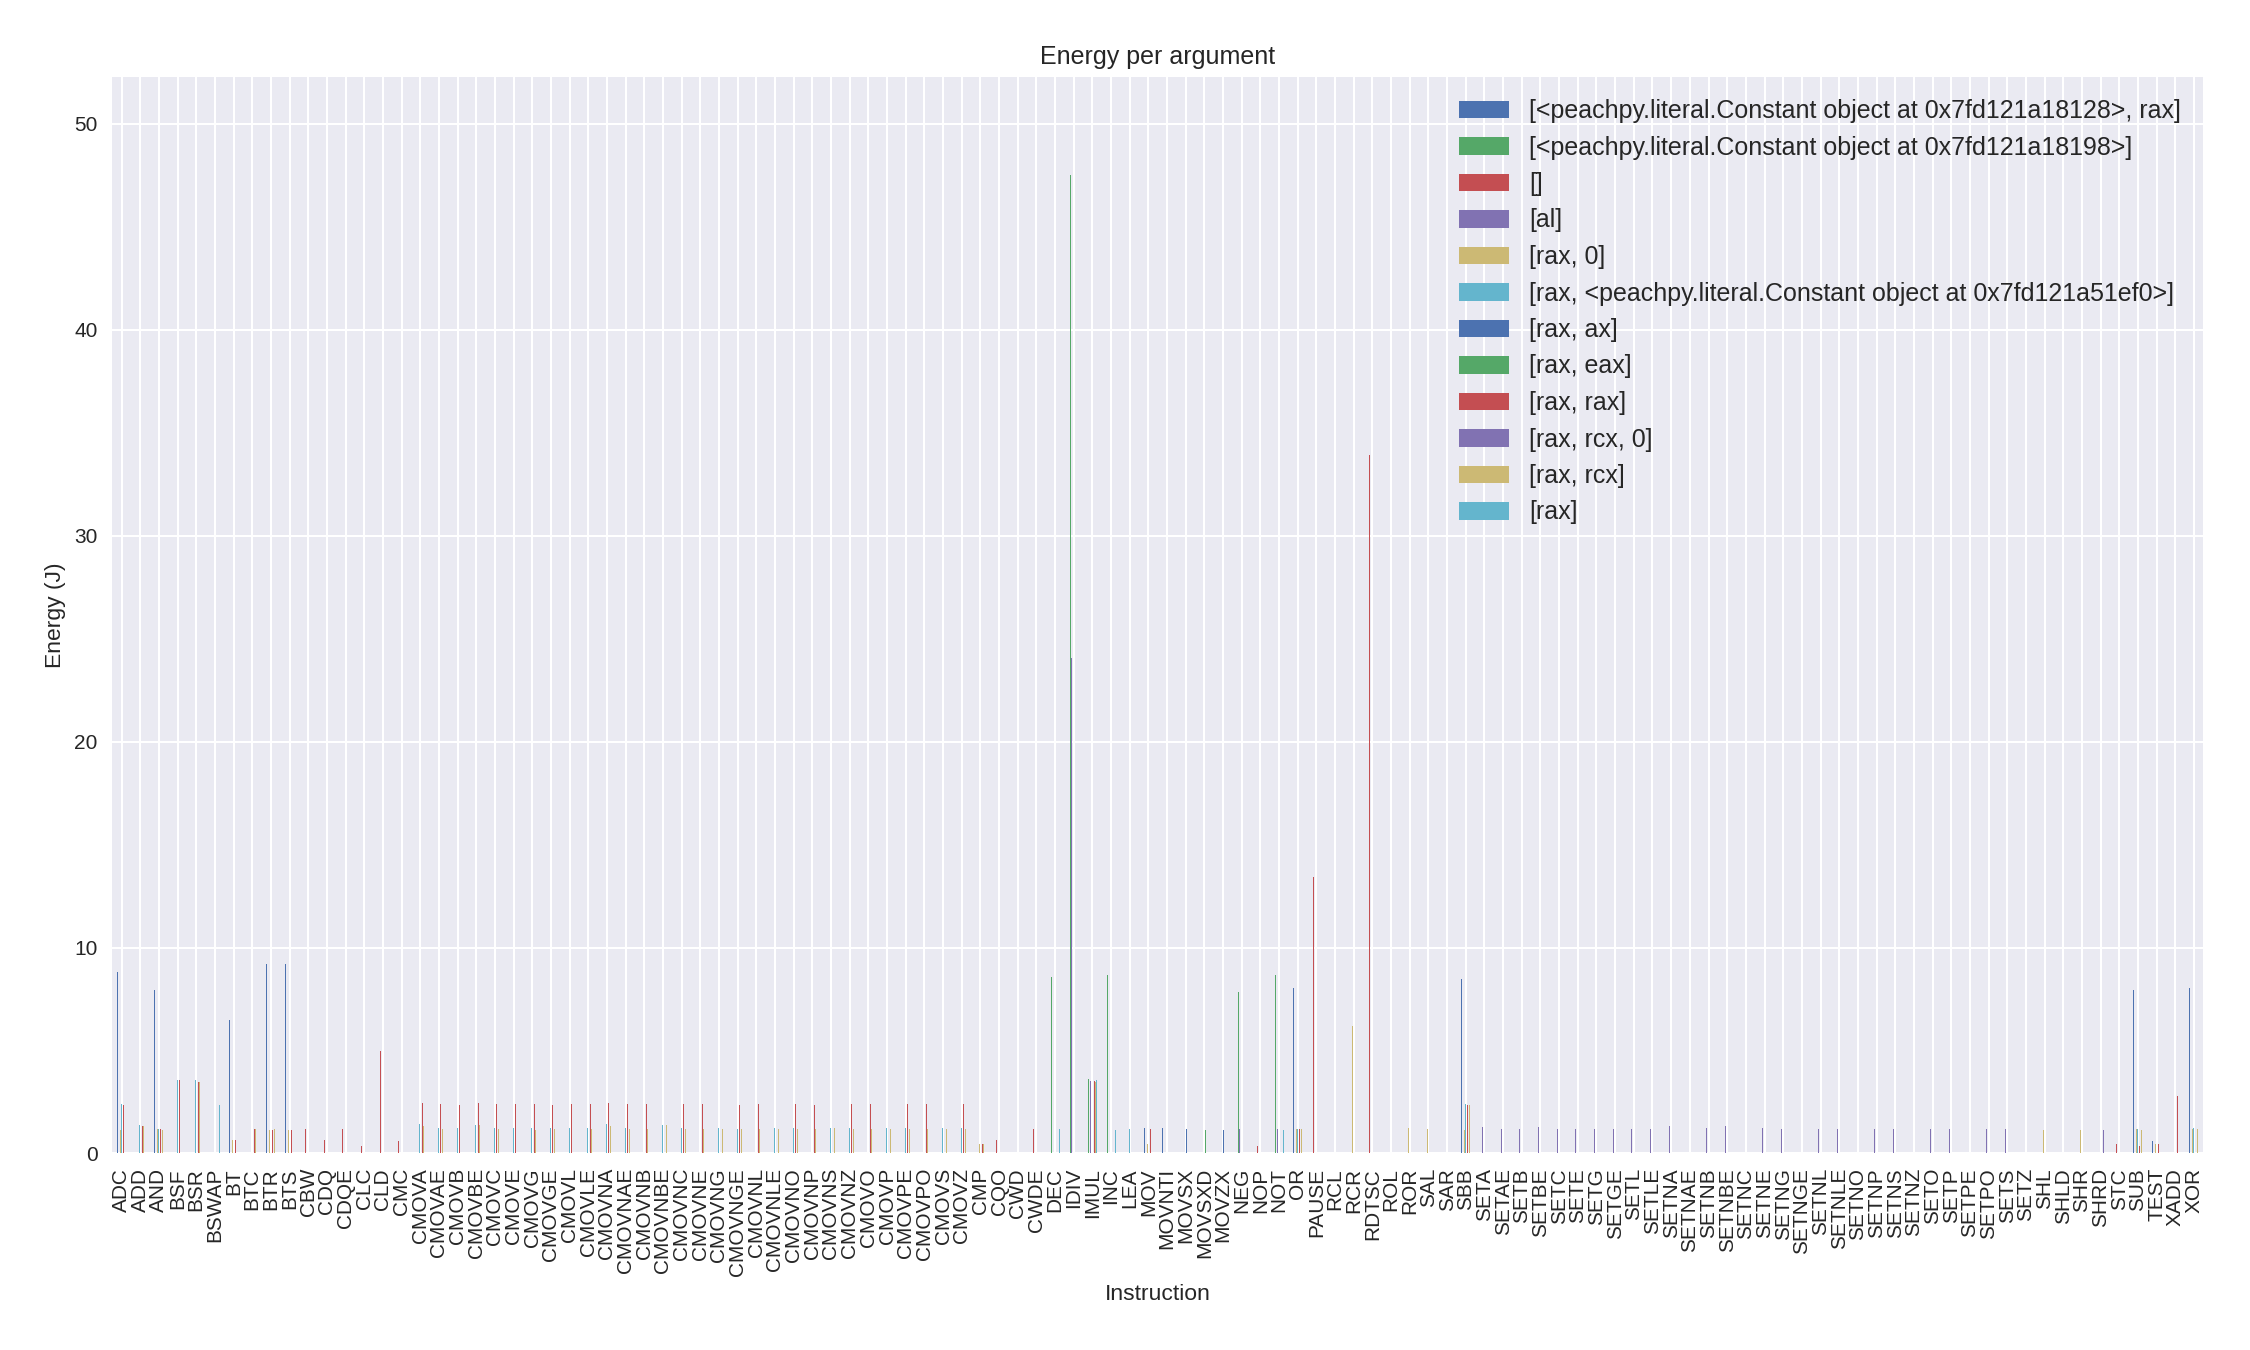
\includegraphics[width=\textwidth]{experiments/figures/inst_en_args_generic.png}
%	\caption{Energy per instruction argument}
%	\label{fig:experiment_en1}
%\end{figure}
%
%\begin{figure}
%	\centering
%	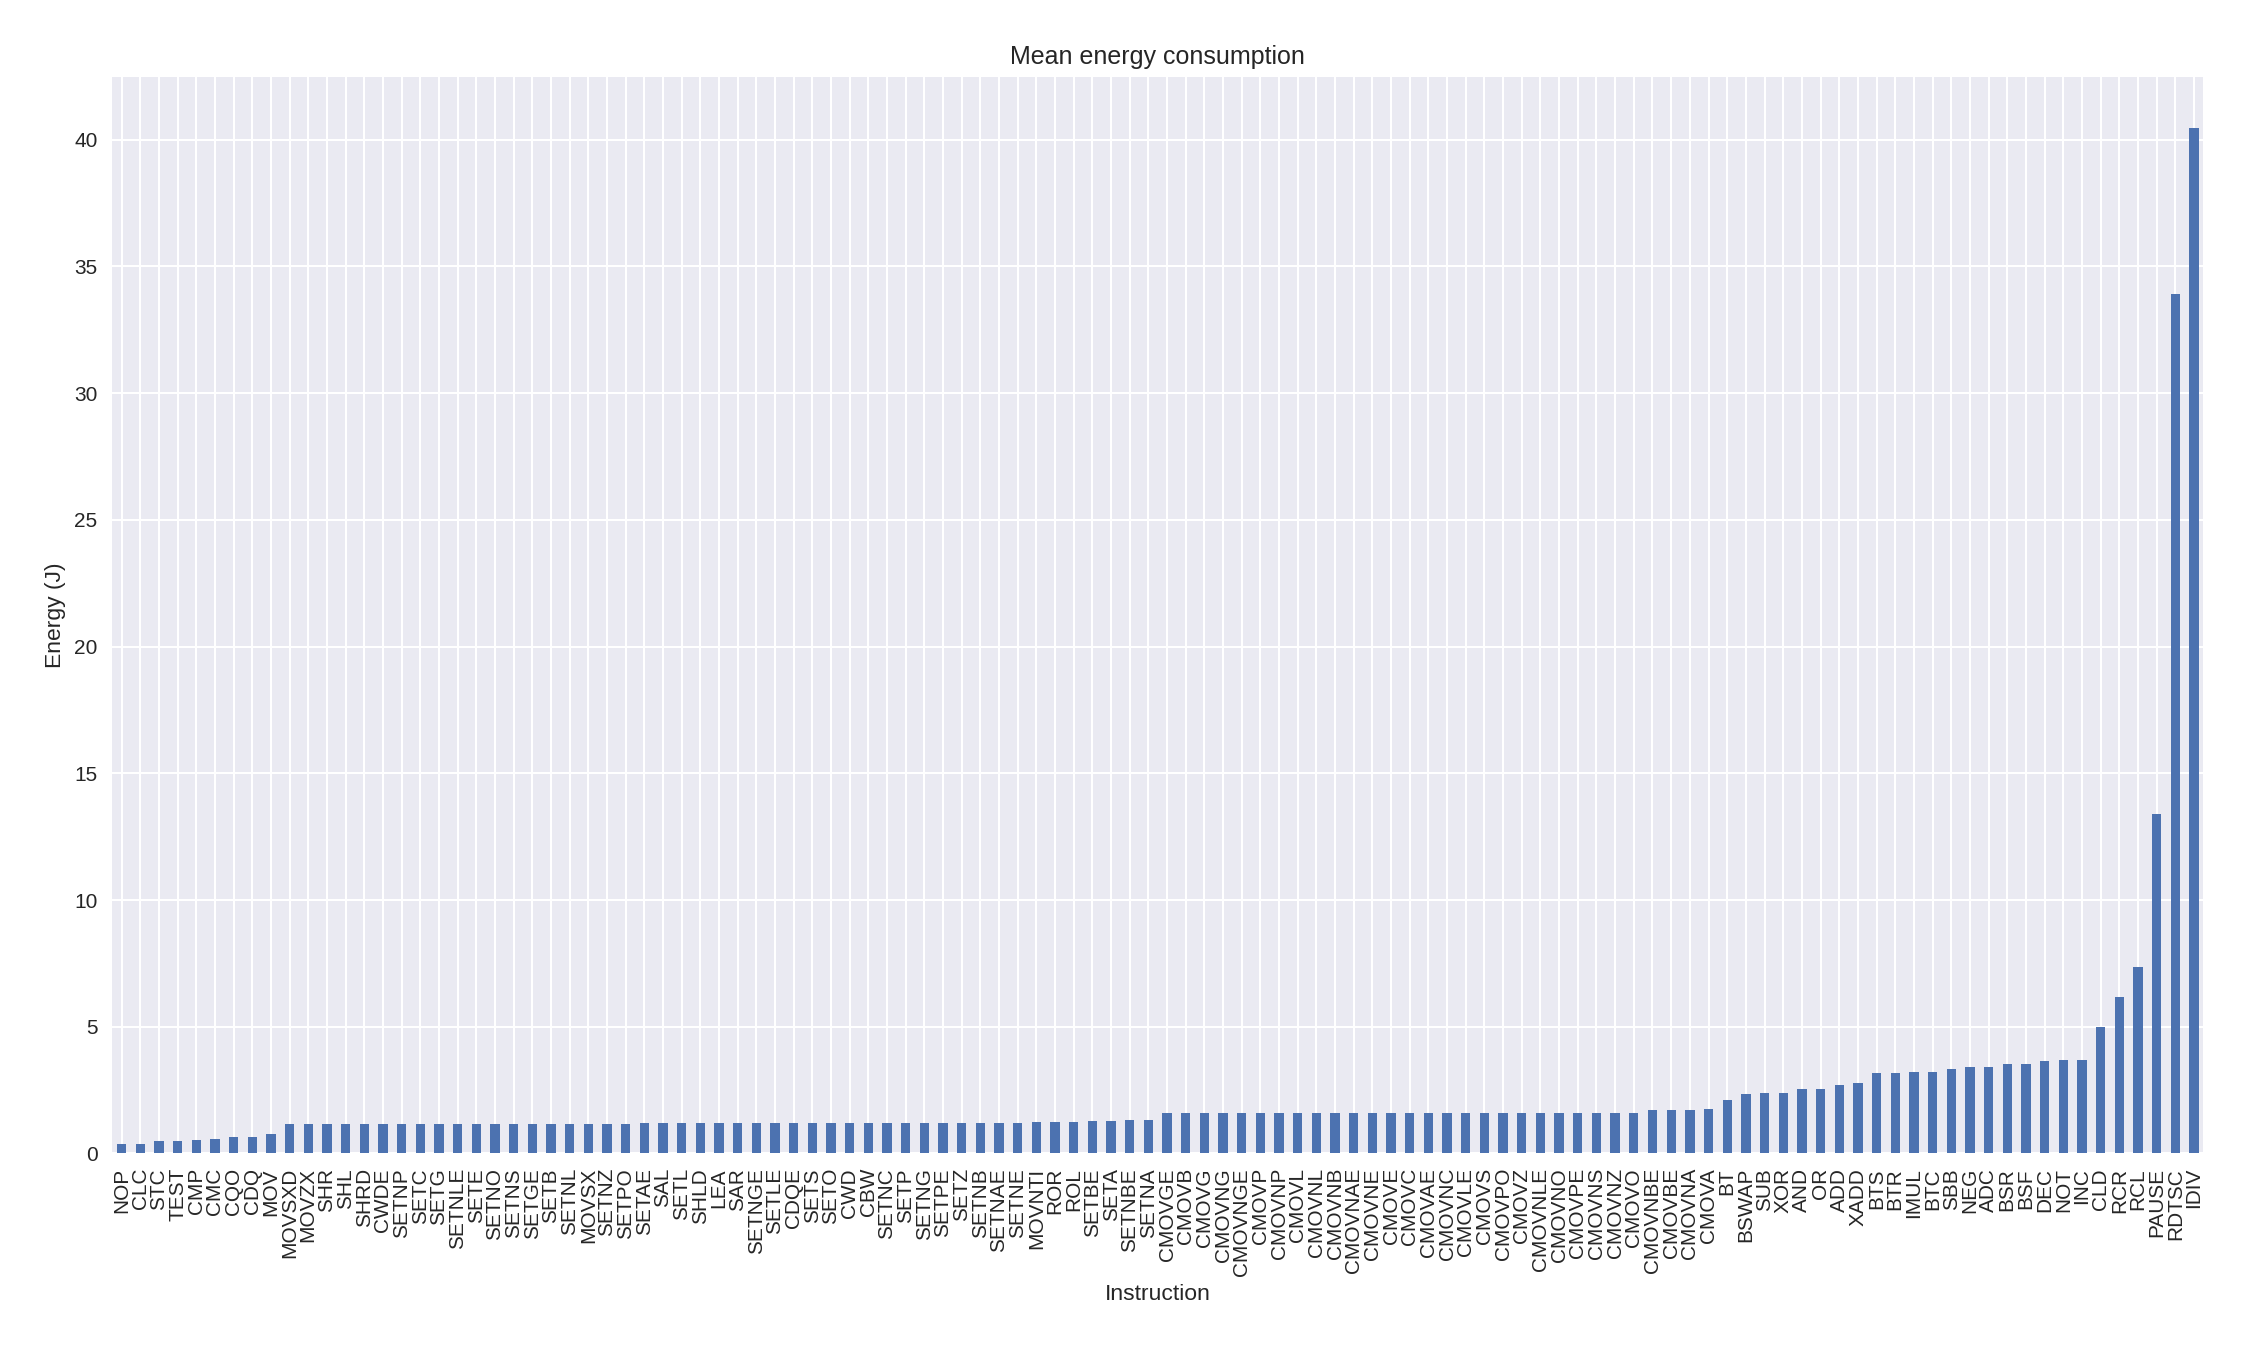
\includegraphics[width=\textwidth]{experiments/figures/inst_mean_en_generic.png}
%	\caption{Mean energy per instruction over all arguments}
%	\label{fig:experiment_en2}
%\end{figure}
%
%\begin{figure}
%	\centering
%	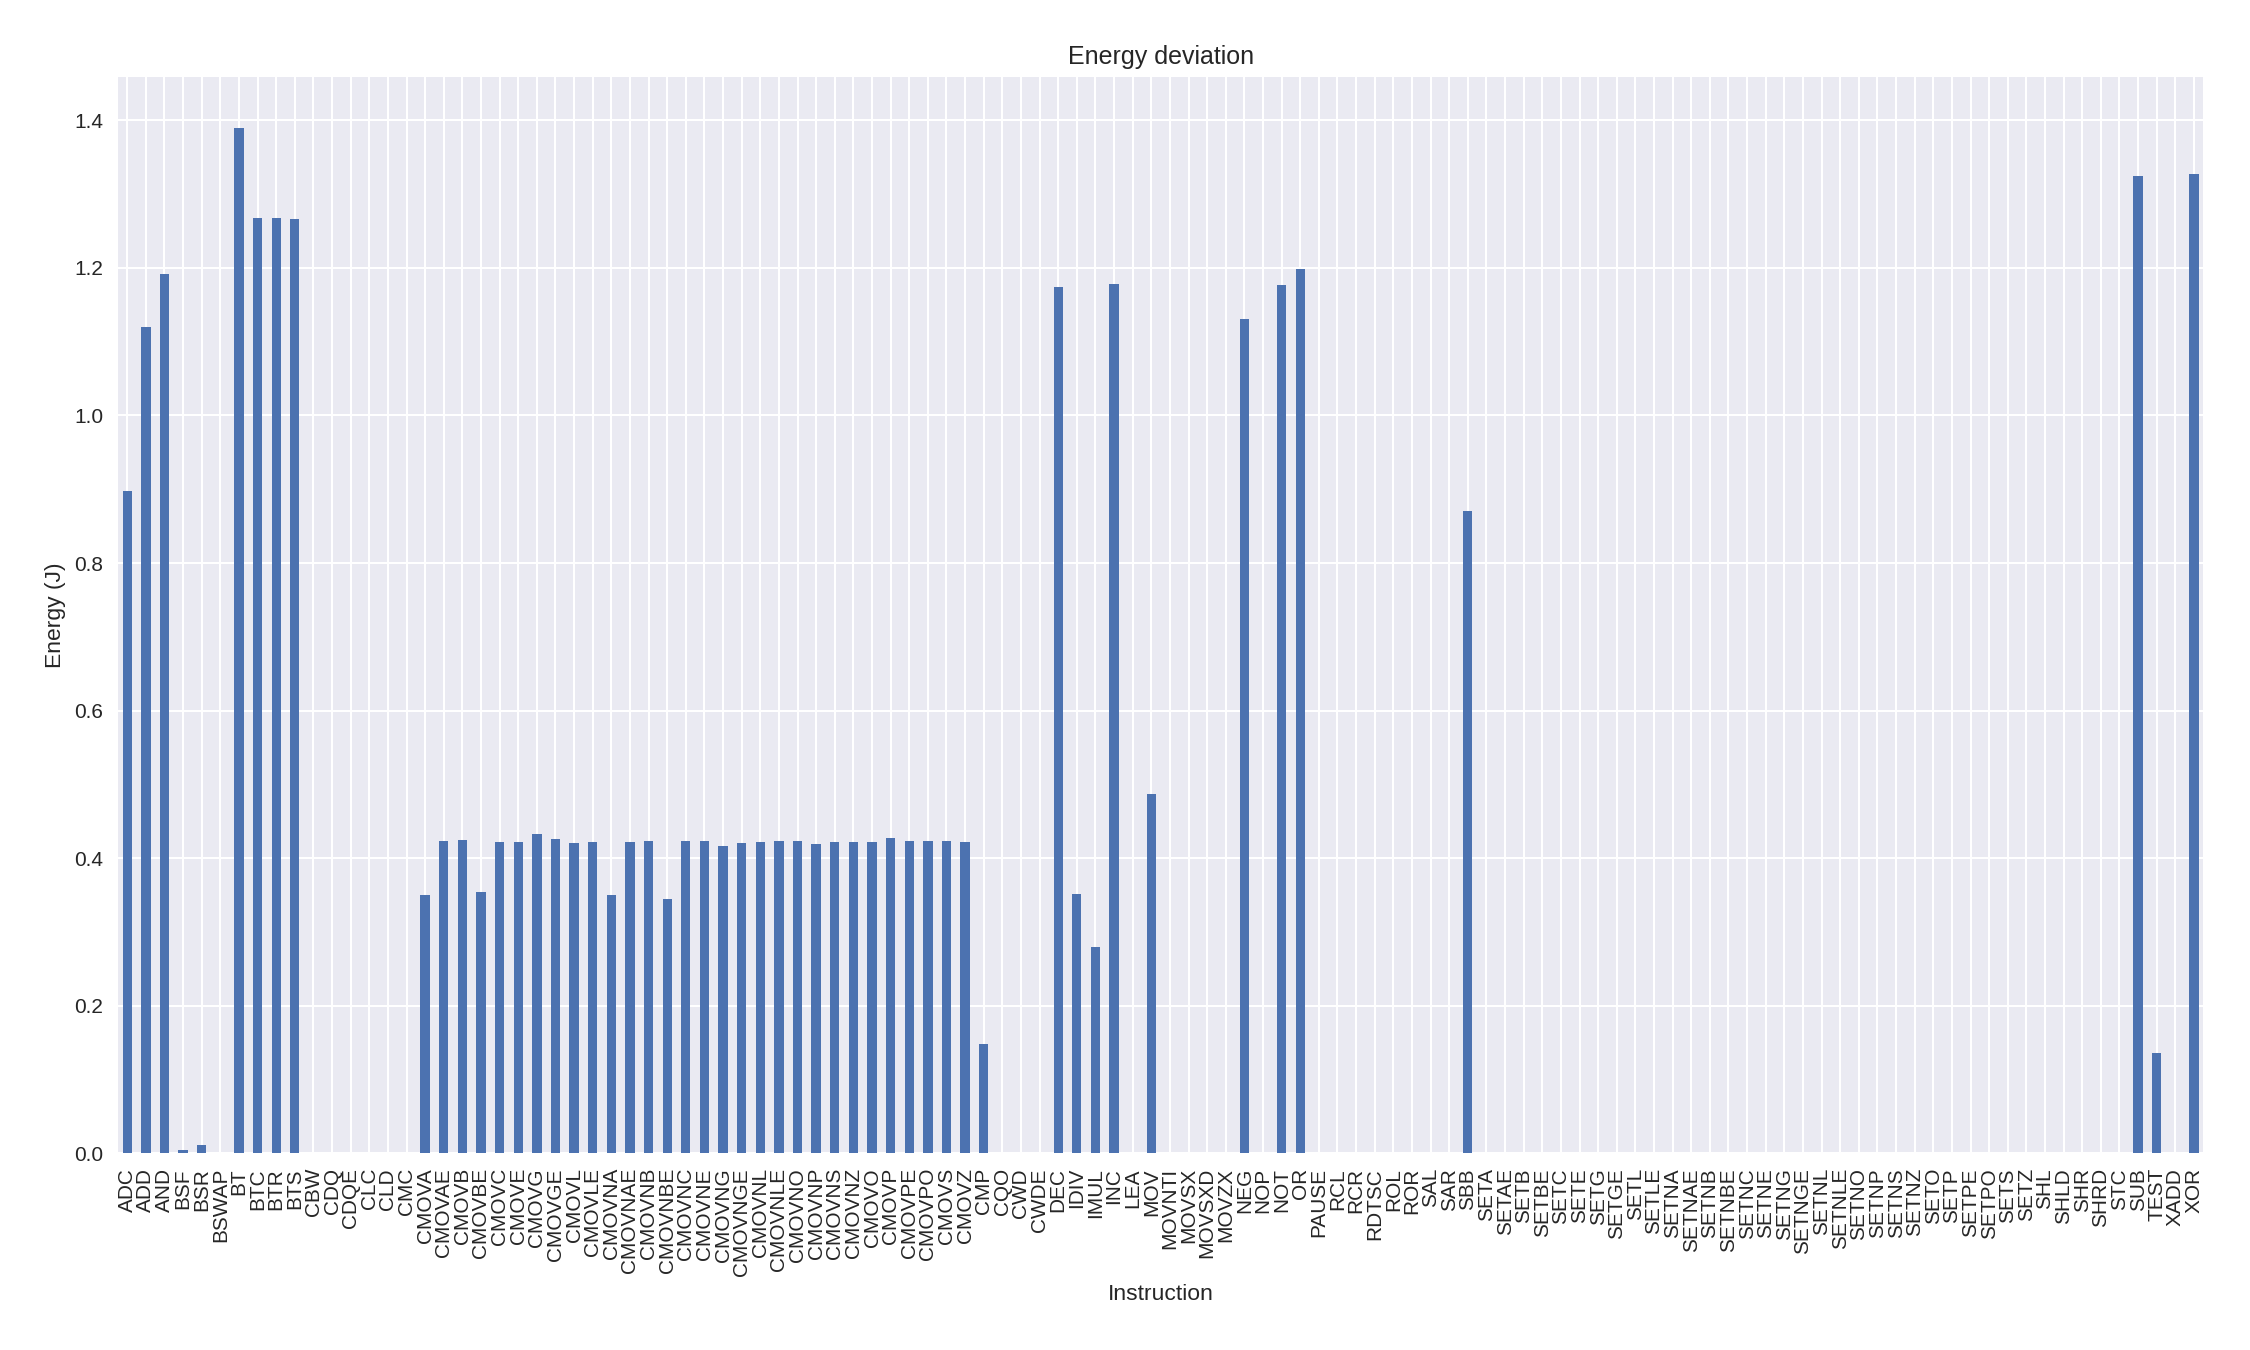
\includegraphics[width=\textwidth]{experiments/figures/inst_std_en_generic.png}
%	\caption{Standard deviation energy per instruction over all arguments}
%	\label{fig:experiment_en3}
%\end{figure}
%
%\subsection{SSE}
%
%\begin{figure}
%	\centering
%	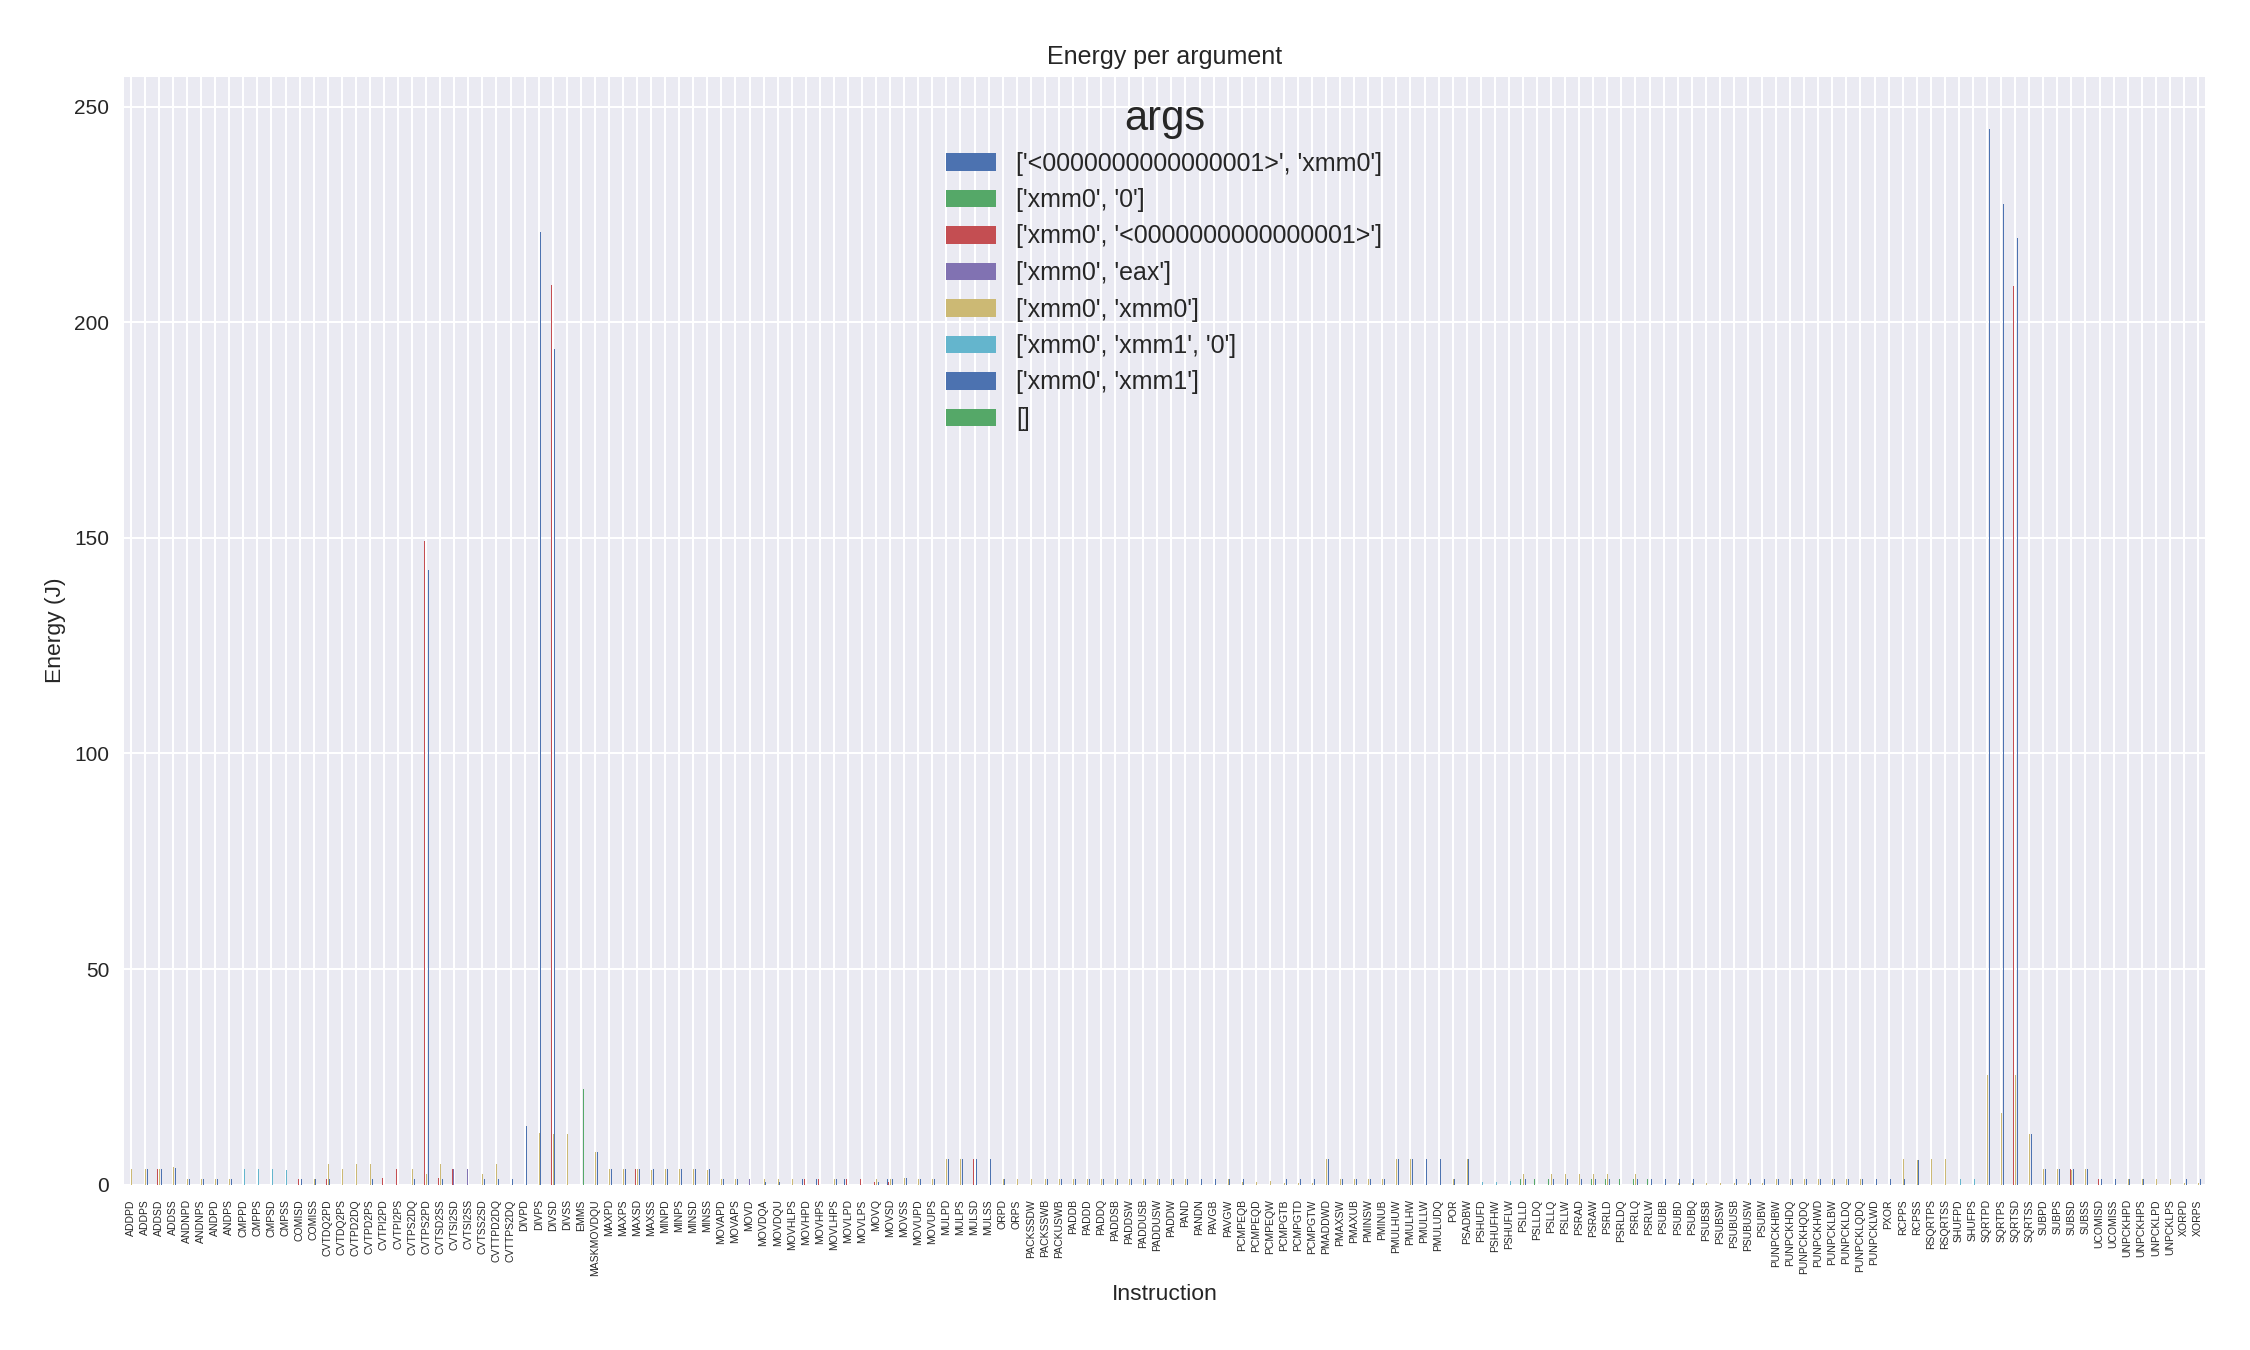
\includegraphics[width=\textwidth]{experiments/figures/inst_en_args_sse.png}
%	\caption{Energy per instruction argument (sse)}
%	\label{fig:experiment_en4}
%\end{figure}
%
%\begin{figure}
%	\centering
%	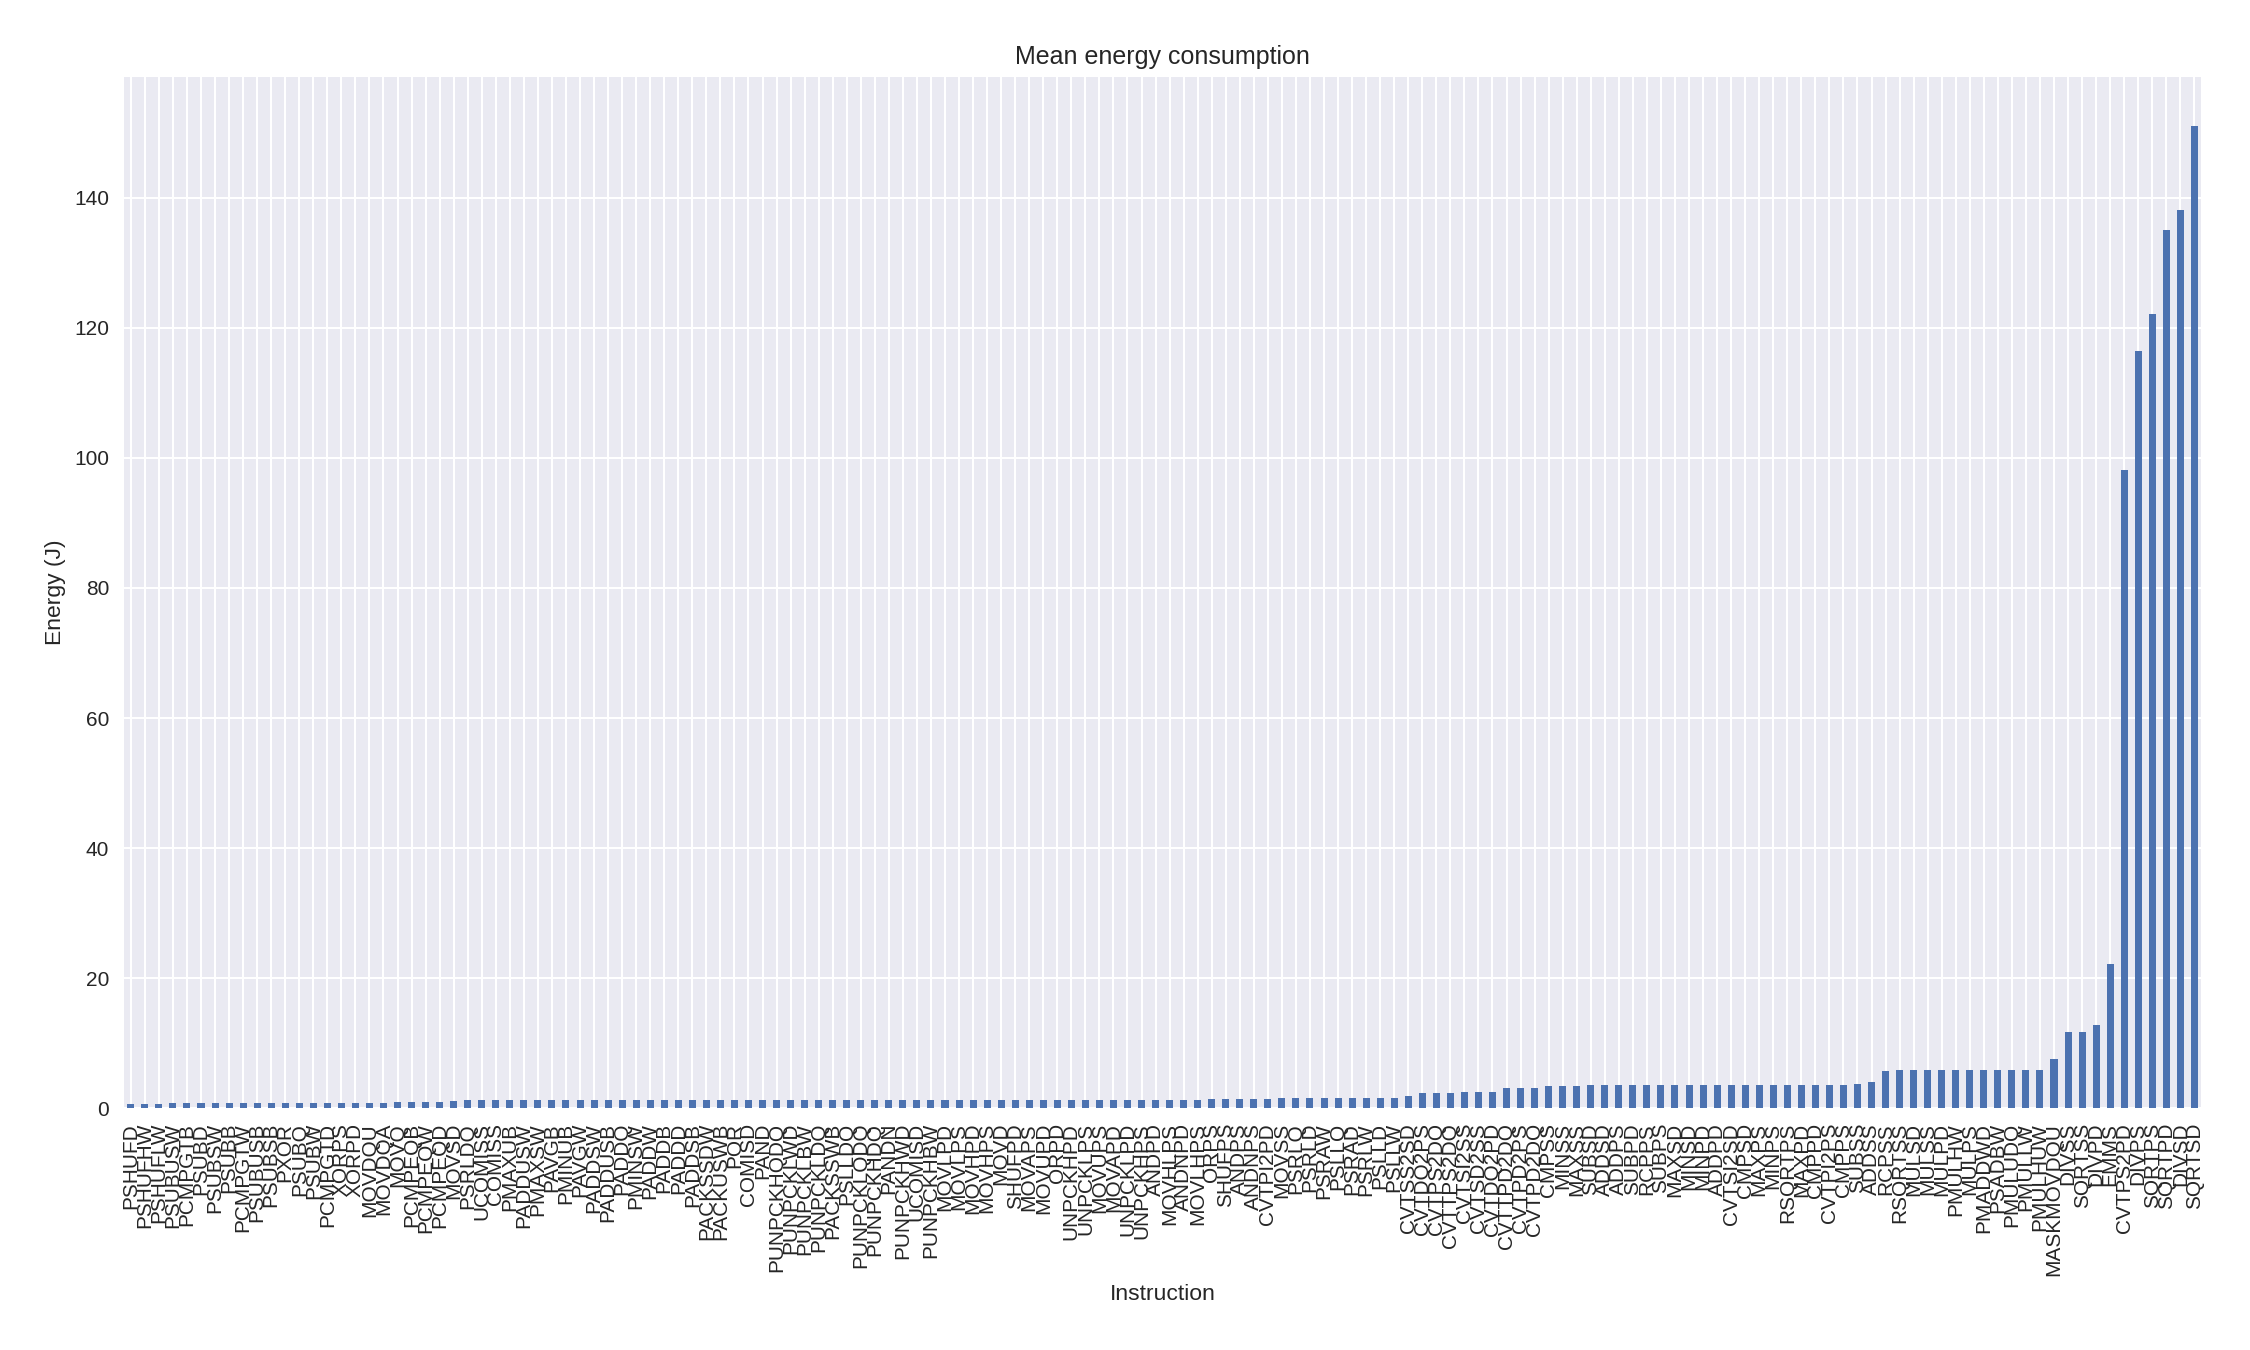
\includegraphics[width=\textwidth]{experiments/figures/inst_mean_en_sse.png}
%	\caption{Mean energy per instruction over all arguments (sse)}
%	\label{fig:experiment_en5}
%\end{figure}
%
%\begin{figure}
%	\centering
%	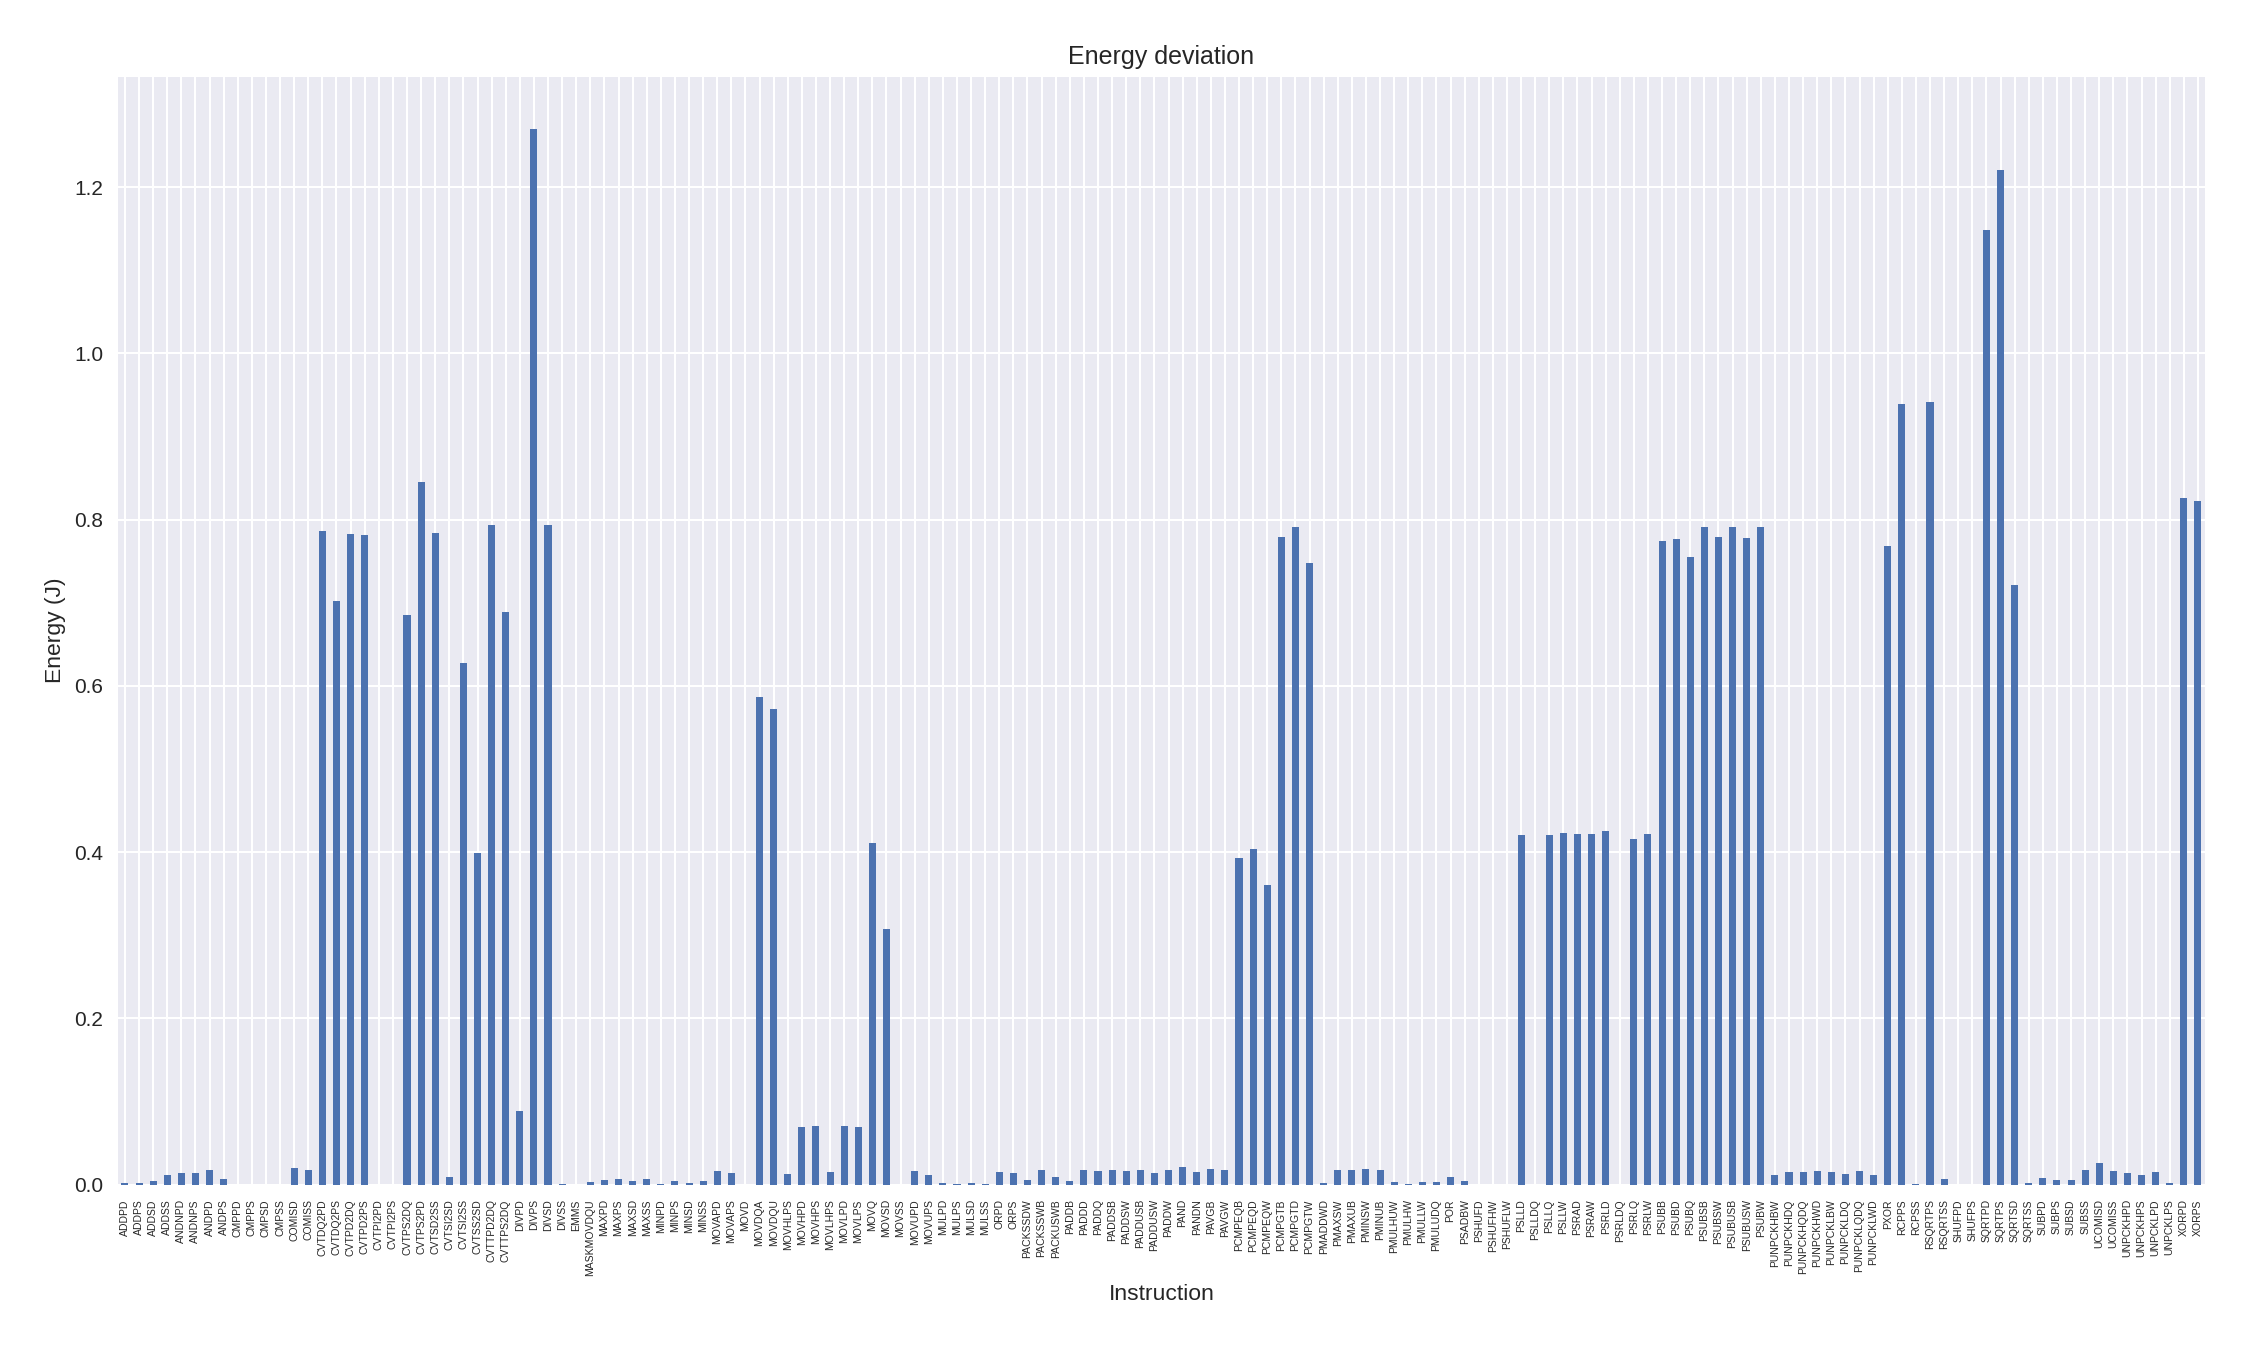
\includegraphics[width=\textwidth]{experiments/figures/inst_std_en_sse.png}
%	\caption{Standard deviation energy per instruction over all arguments (sse)}
%	\label{fig:experiment_en6}
%\end{figure}
%
%\subsection{SSE and Generic}
%
%\begin{figure}
%	\centering
%	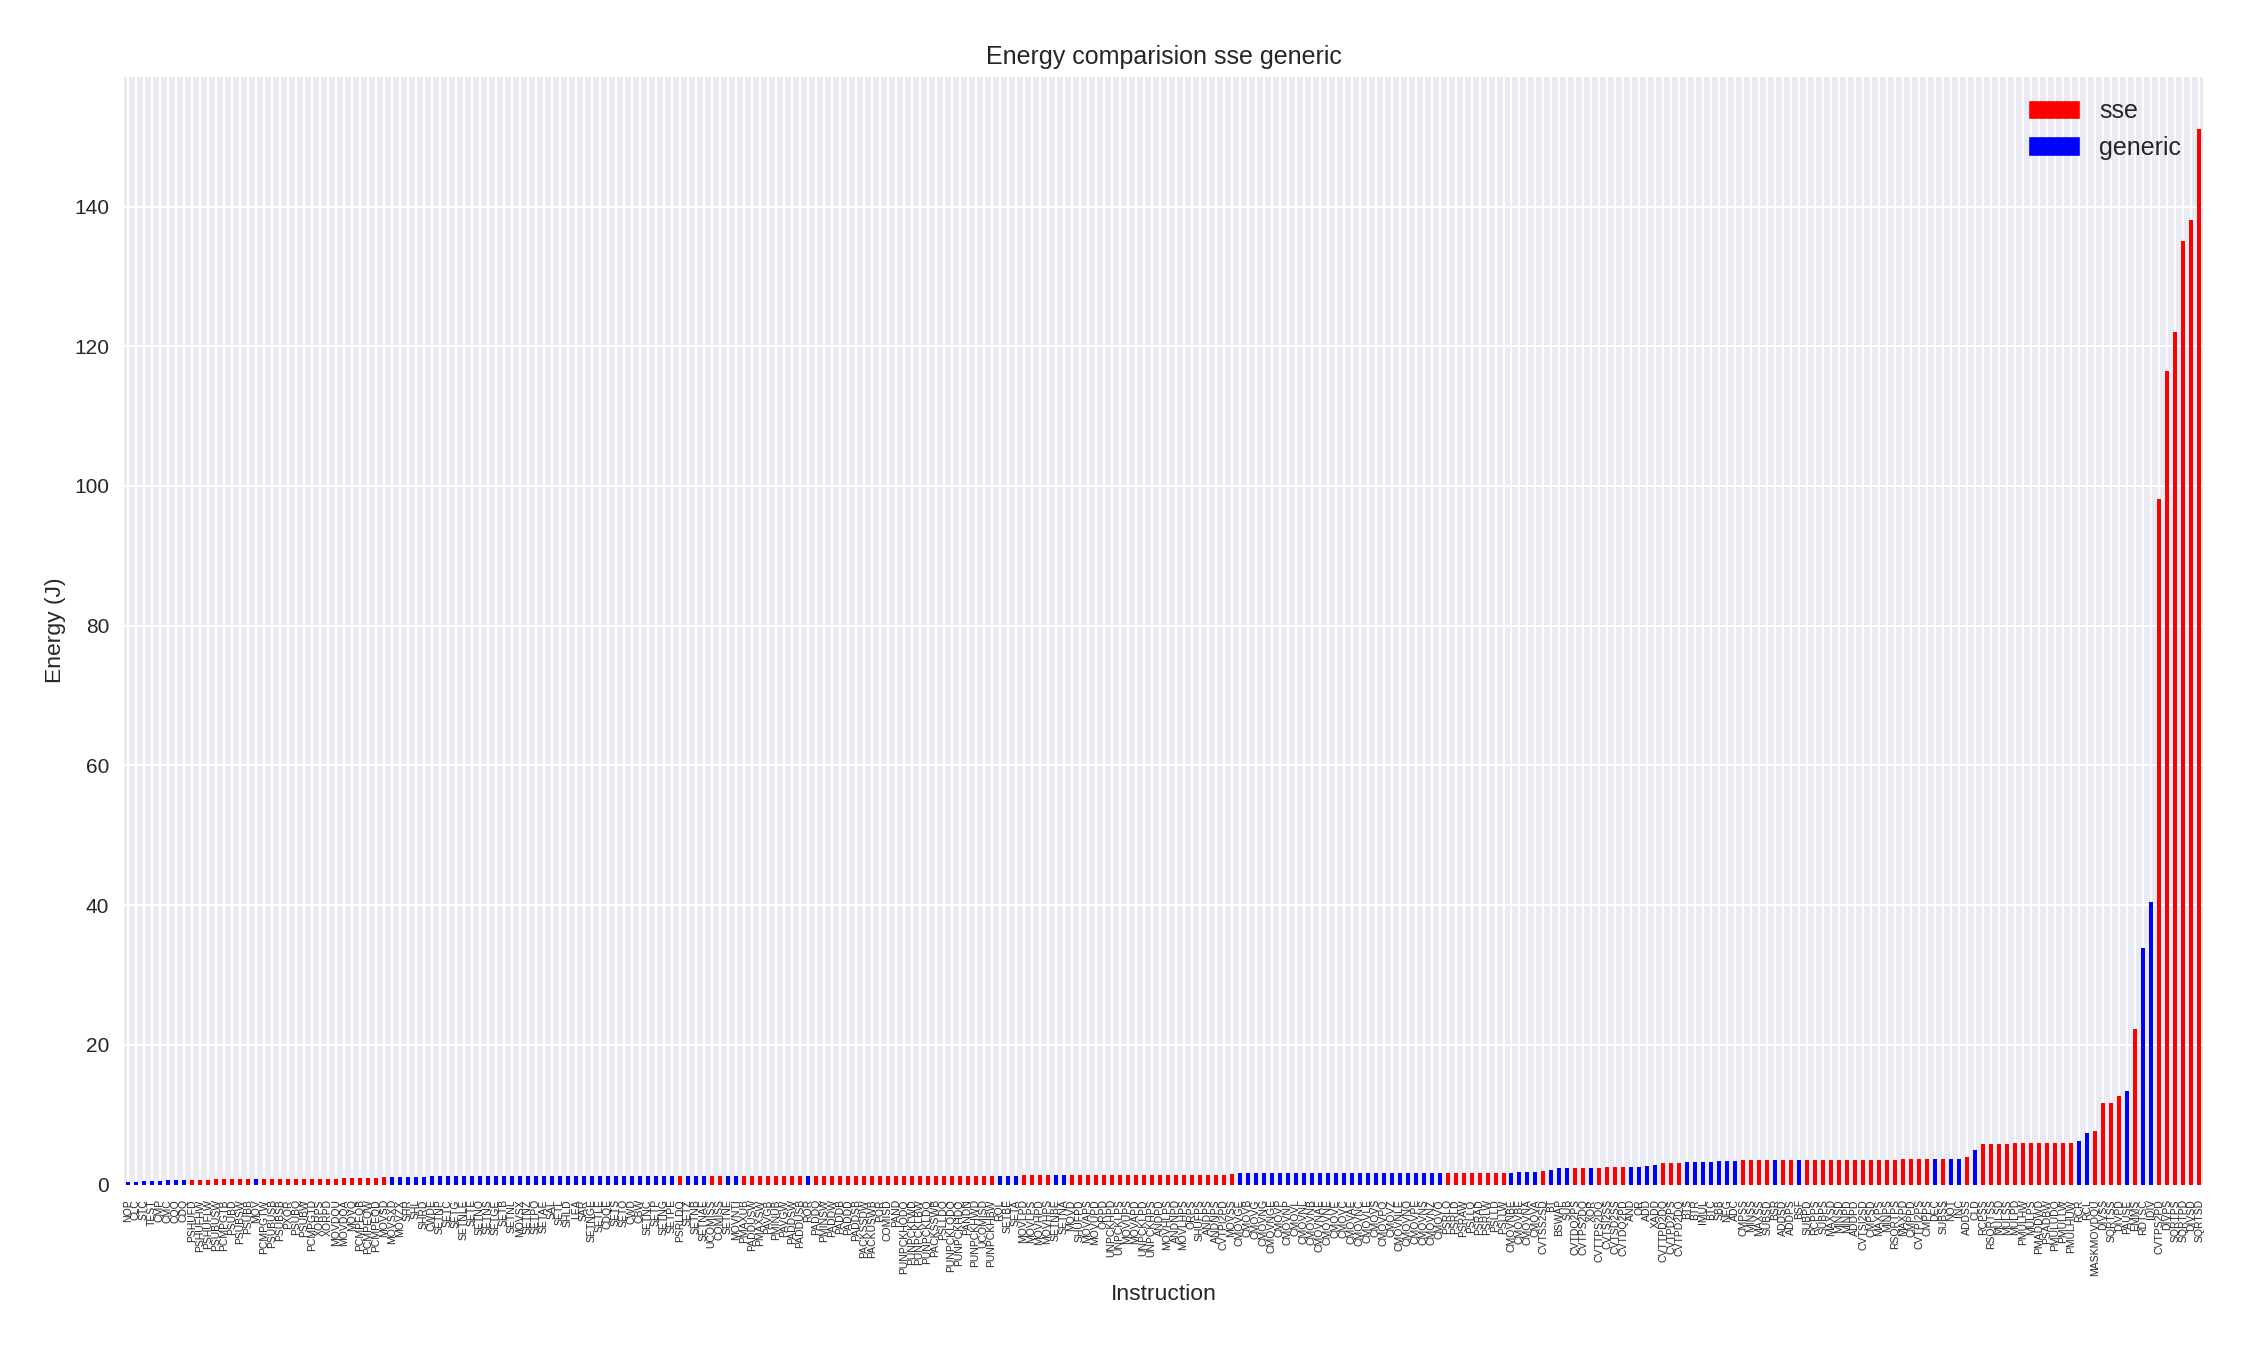
\includegraphics[width=\textwidth]{experiments/figures/inst_en_cmp_sse_generic.png}
%	\caption{Comparing SSE and generic instructions energy consumption}
%	\label{fig:experiment_en7}
%\end{figure}
%
%\subsection{Power}
%
%\begin{figure}
%	\centering
%	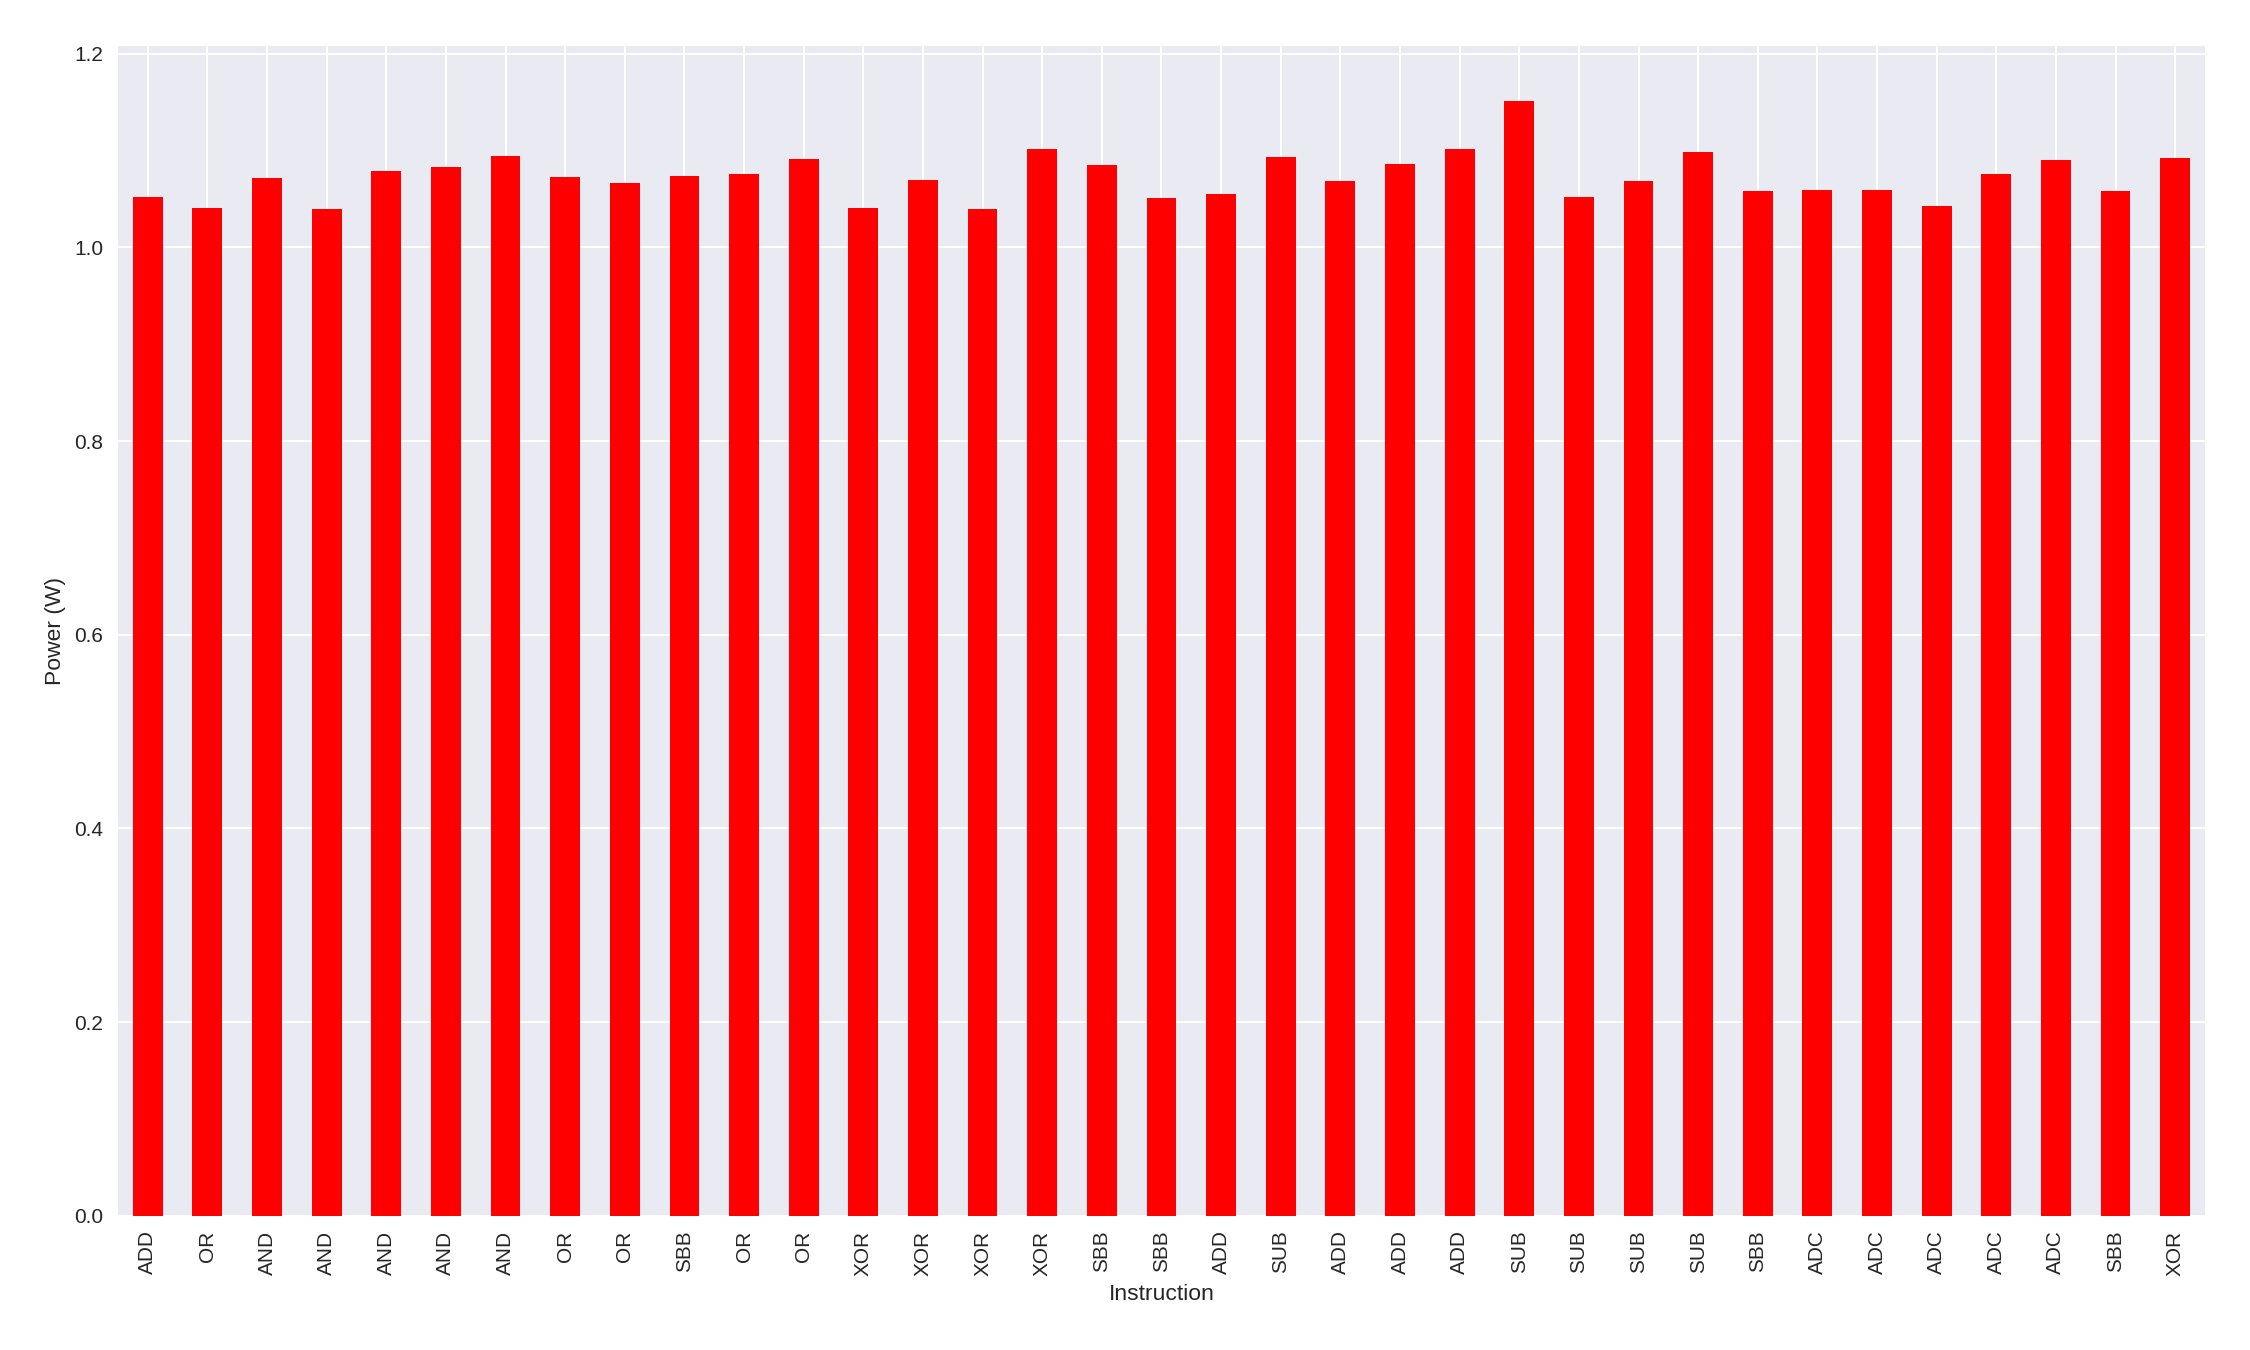
\includegraphics[width=\textwidth]{experiments/figures/inst_pw_generic.png}
%	\caption{Instructions power draw}
%	\label{fig:experiment_pw1}
%\end{figure}
%\begin{figure}
%	\centering
%	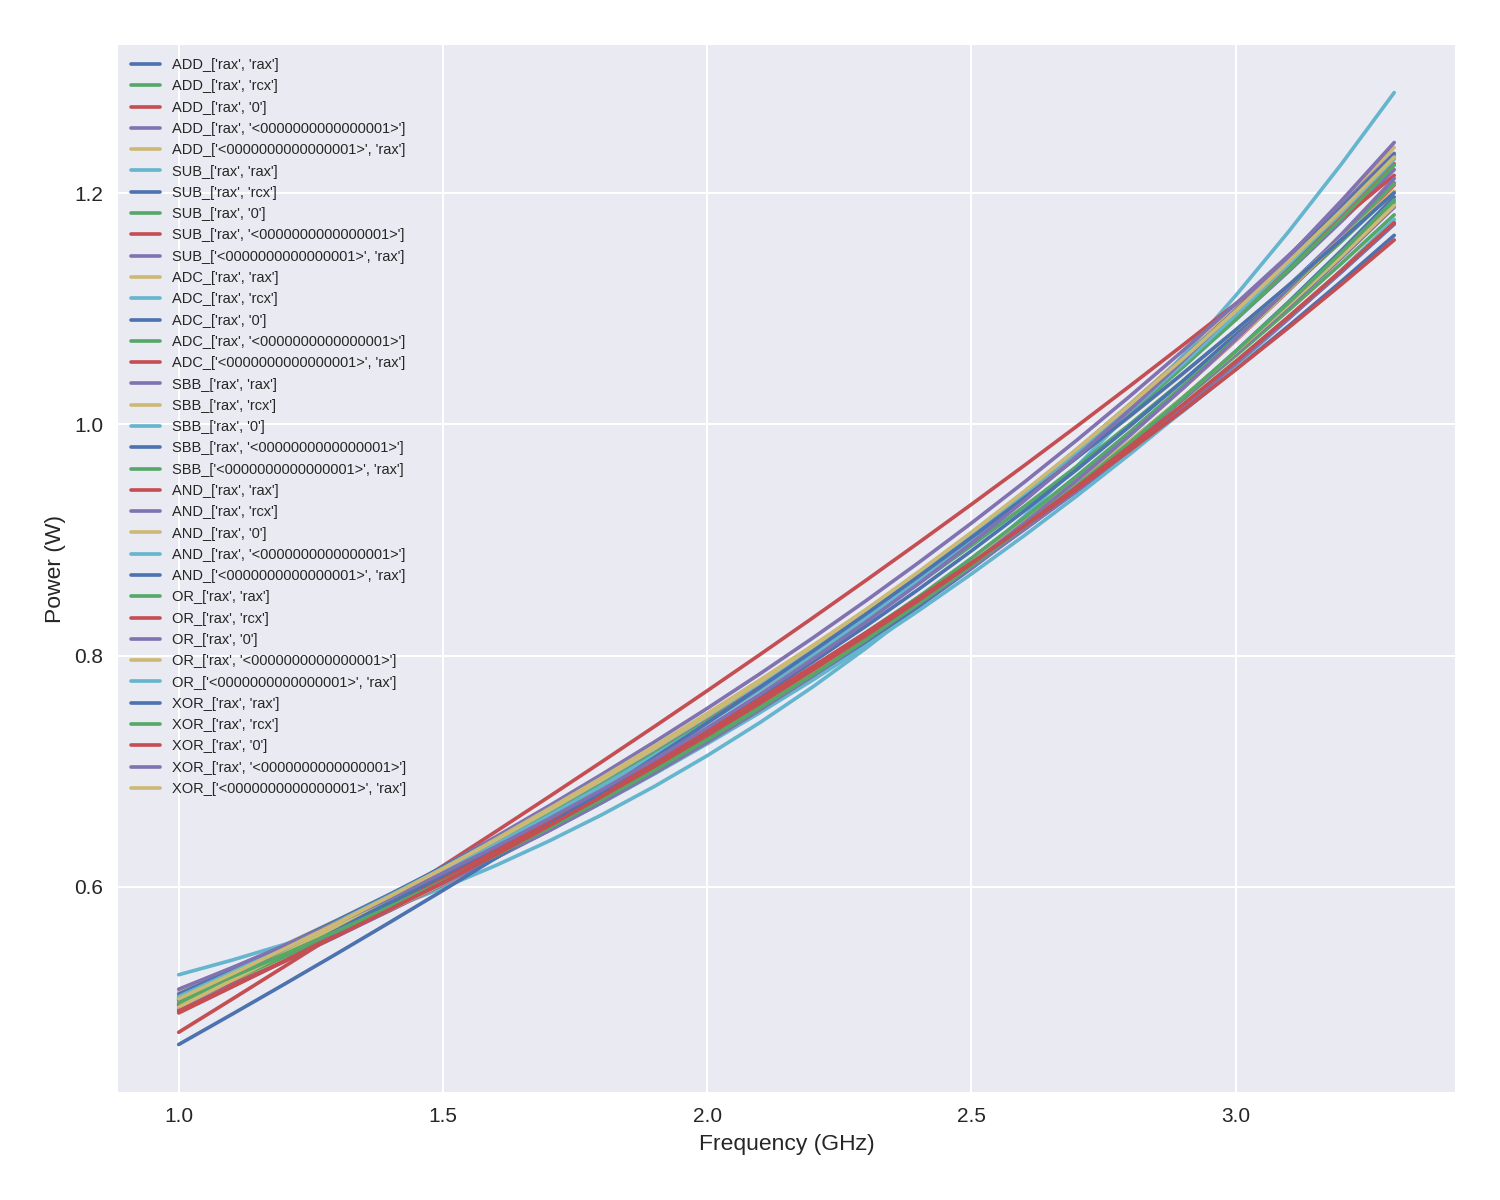
\includegraphics[width=\textwidth]{experiments/figures/inst_pw_args.png}
%	\caption{Instructions power draw by argument}
%	\label{fig:experiment_pw2}
%\end{figure}
%
%\section{Tracing application methods}
%
%\begin{outline}
%	\1 Linux ptrace
%		\2 Breakpoint on each instruction	
%	\1 Intel pin
%		\2 JIT
%		\2 Not open source
%	\1 qemu user
%		\2 TCG accelerator (transform target to host instruction) similar to JIT
%		\2 Partial emulation
%\end{outline}
%
%We choose the less intrusive and open-source alternative qemu user, with an small modificaion we are able to trace an application instructions. Generating an table as follows:
%
%
%\begin{table}[H]
%	\centering
%	\begin{tabular}{|c|c|c|}
%		\hline
%		opcode         & mnemonic & args                          \\ \hline
%		48 89 e7       & movq     & \%rsp, \%rdi\textbackslash{}n \\ \hline
%		48 89 e7       & movq     & \%rsp, \%rdi\textbackslash{}n \\ \hline
%		e8 08 0e 00 00 & callq    & 0x4000a24ea0\textbackslash{}n \\ \hline
%		55             & pushq    & \%rbp\textbackslash{}n        \\ \hline
%		48 89 e5       & movq     & \%rsp, \%rbp\textbackslash{}n \\ \hline
%		41 57          & pushq    & \%r15\textbackslash{}n        \\ \hline
%		41 56          & pushq    & \%r14\textbackslash{}n        \\ \hline
%		41 55          & pushq    & \%r13\textbackslash{}n        \\ \hline
%		& \vdots & \\ \hline
%	\end{tabular}
%\end{table}
%
%
%\section{CPU load}
%
%\begin{figure}[H]
%	\centering
%	\begin{subfigure}[b]{0.45\textwidth}
%		\centering
%		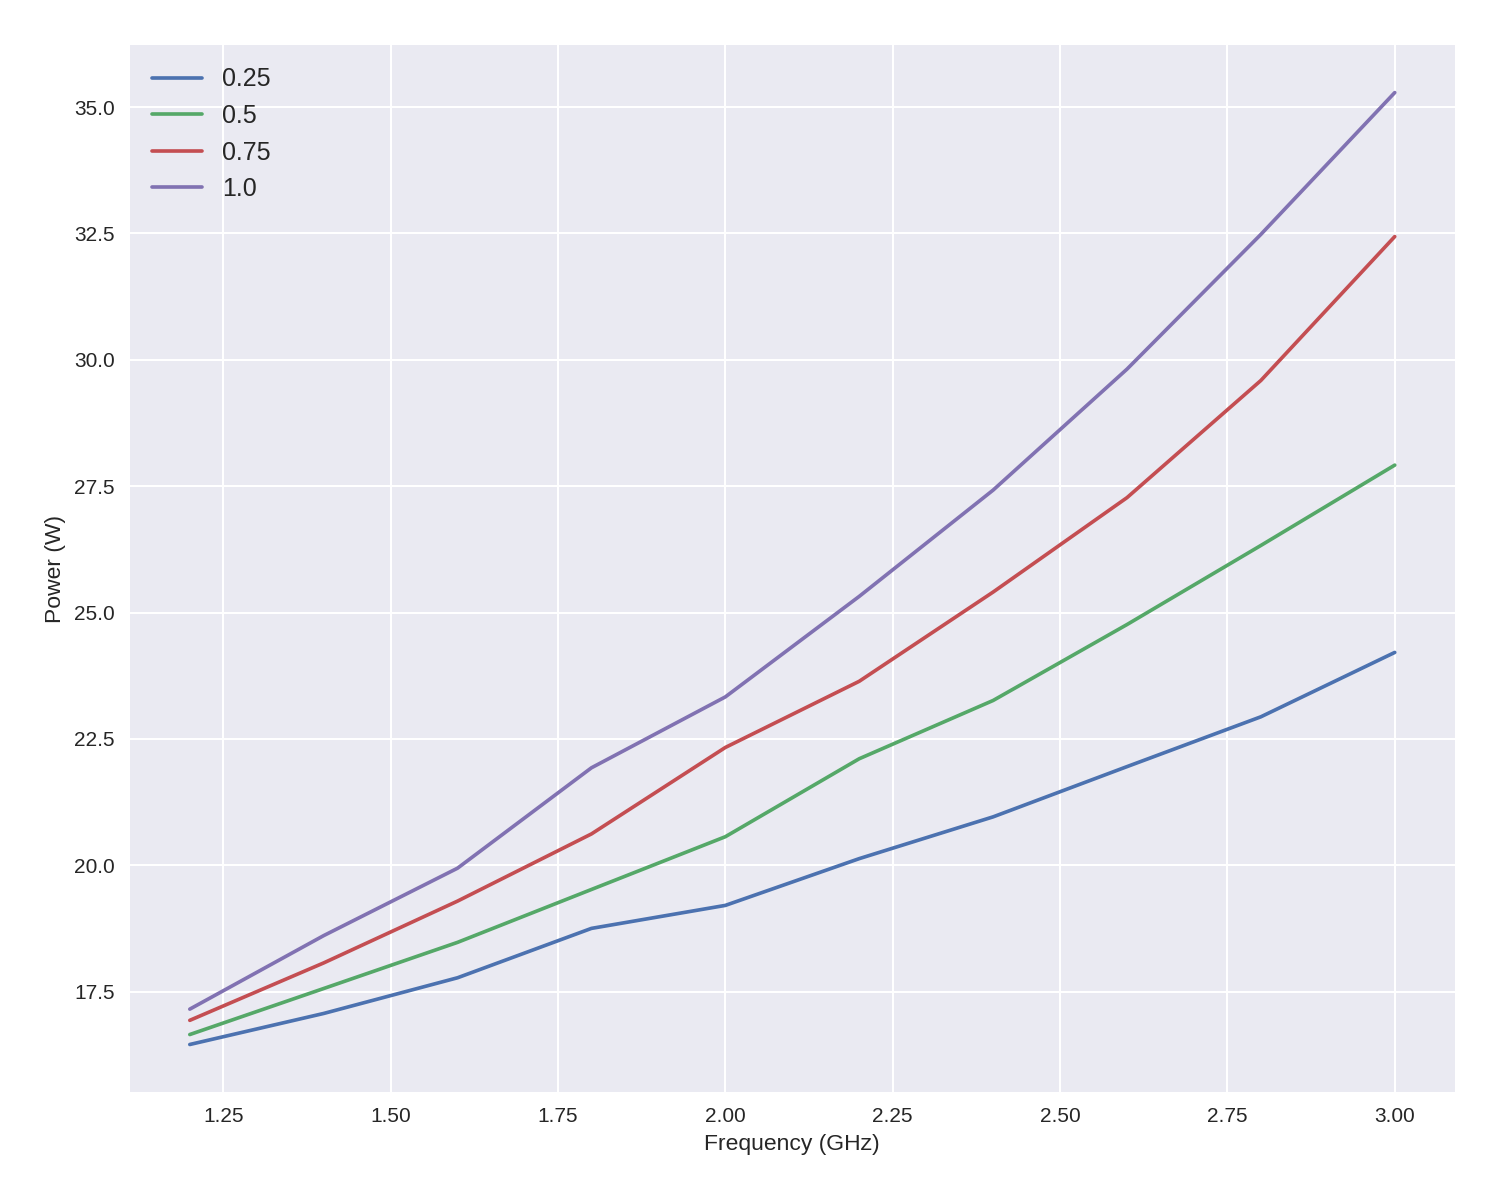
\includegraphics[width=1\columnwidth]{experiments/figures/pw_freq_load.png}
%		\caption{Instructions power draw varing CPU load}
%		\label{fig:experiment_pw_load}
%	\end{subfigure}
%	%
%	\begin{subfigure}[b]{0.45\textwidth}
%		\centering
%		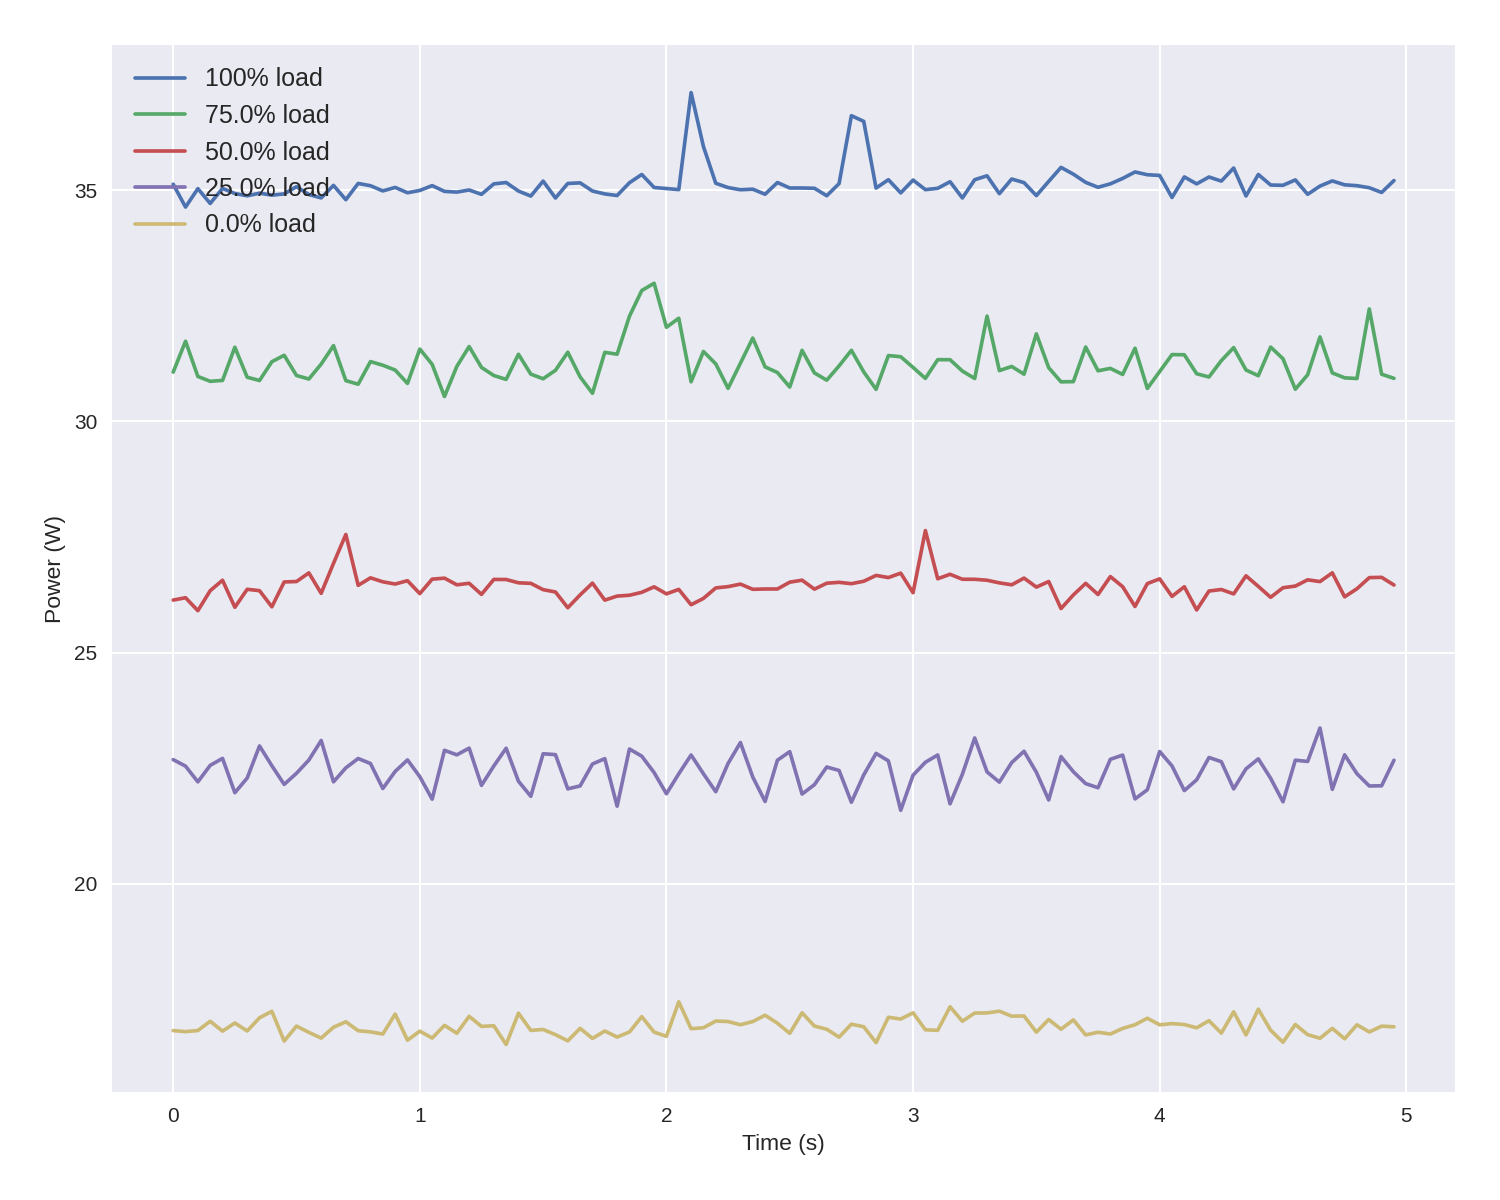
\includegraphics[width=1\columnwidth]{experiments/figures/pw_load.png}
%		\caption{Instructions power draw varing CPU load}
%		\label{fig:experiment_pw_load}
%	\end{subfigure}
%\end{figure}
%
%
%\section{Analysis}
%
%\subsection{Pareto points}

%
%\begin{figure}

%	\centering

%	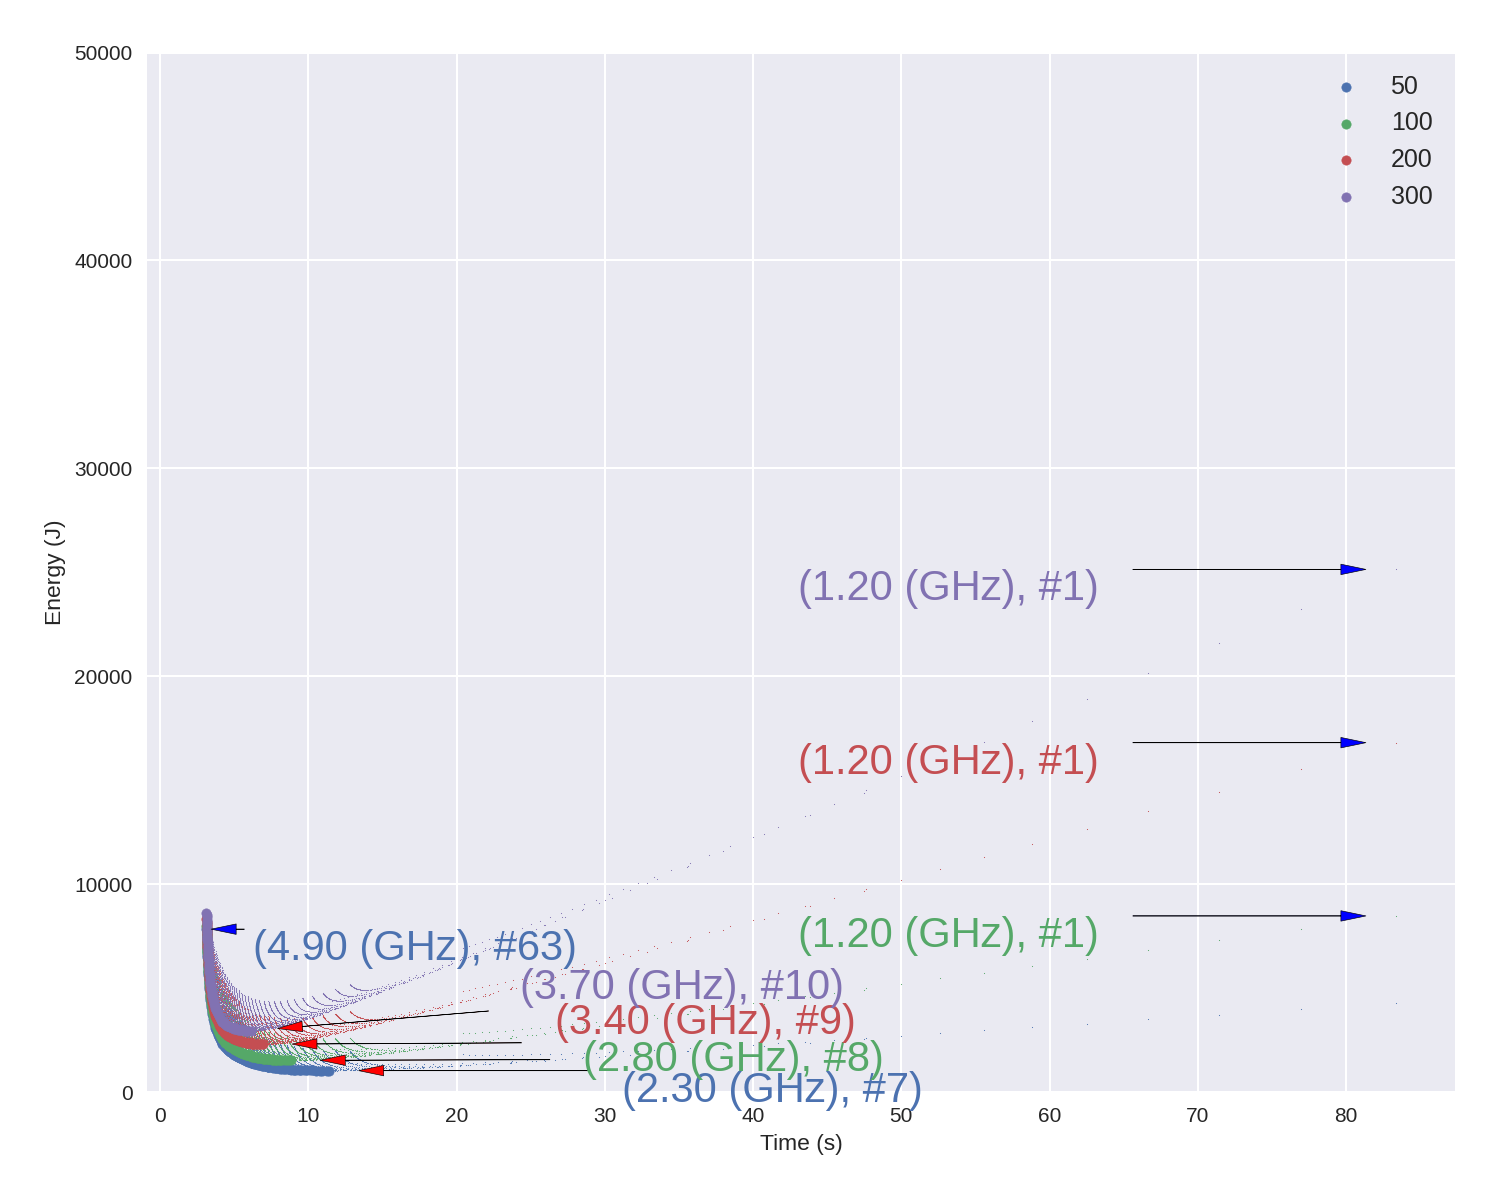
\includegraphics[width=\columnwidth]{models/figures/analisys/pareto_static_high.png}

%	\caption{Pareto static energy}

%	\label{fig:pareto_static_h}

%\end{figure}

%
%
%\begin{figure}

%	\centering

%	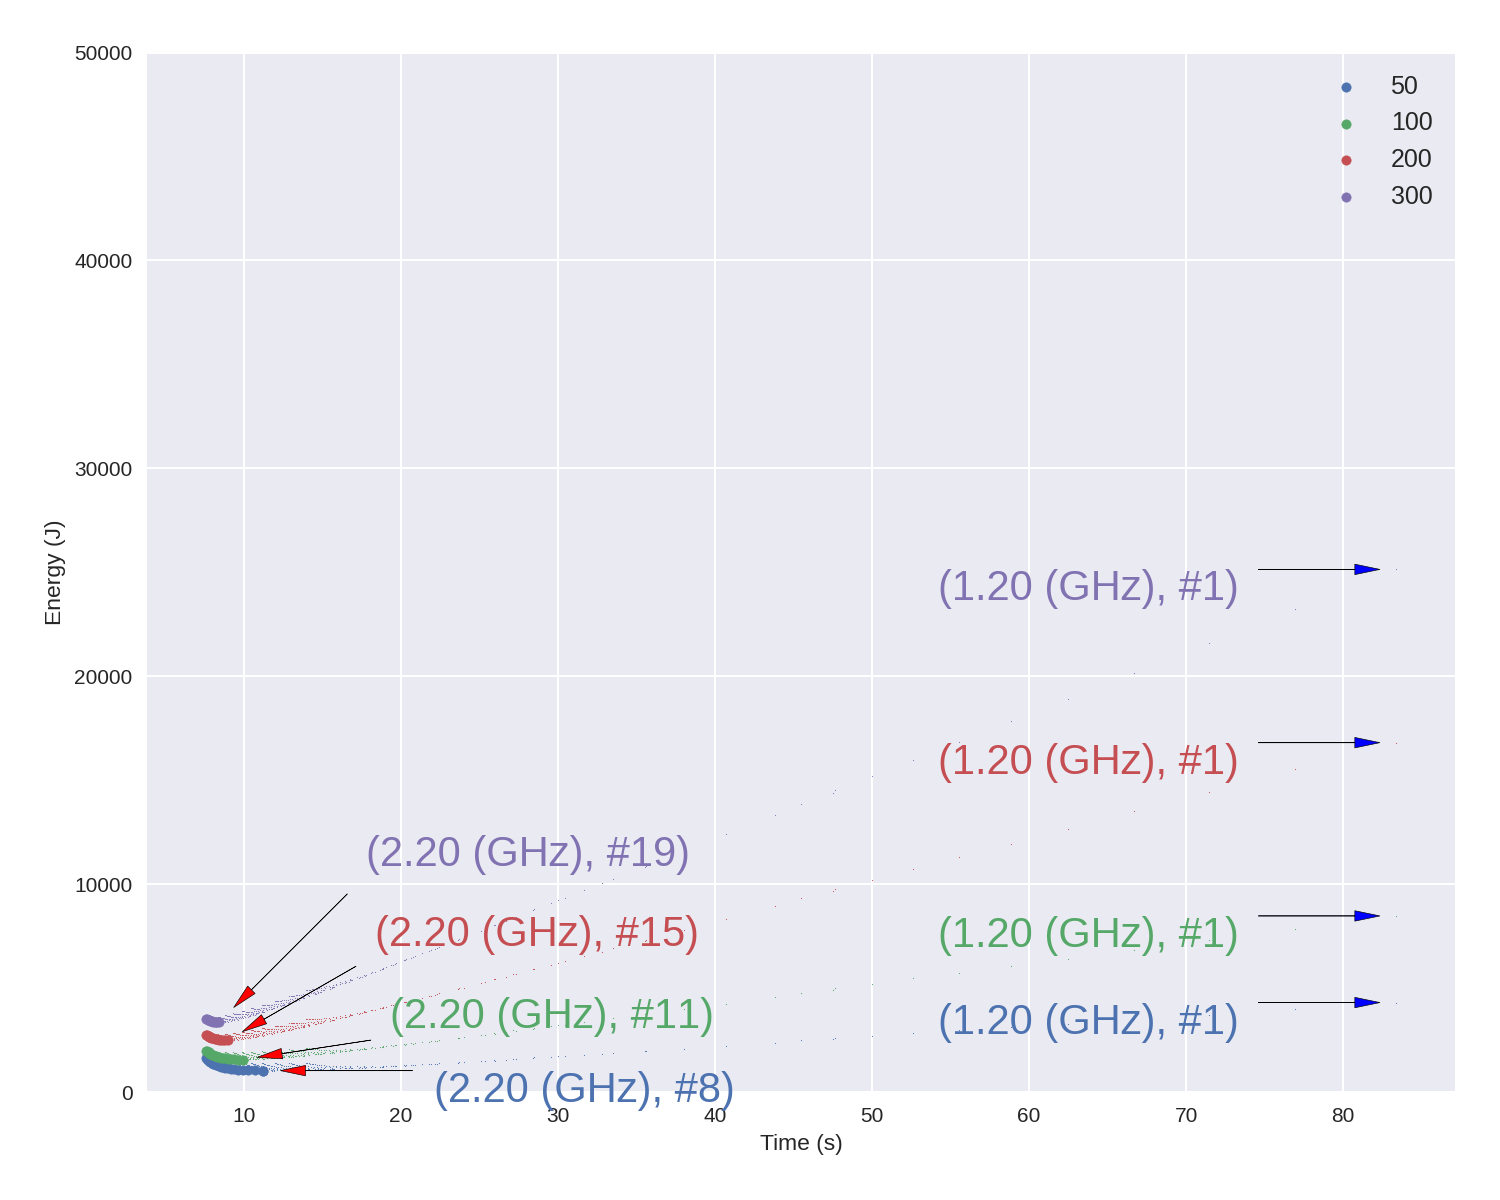
\includegraphics[width=\columnwidth]{models/figures/analisys/pareto_static_low.png}

%	\caption{Pareto static energy}

%	\label{fig:pareto_static_l}

%\end{figure}

%
%
%\begin{figure}

%	\centering

%	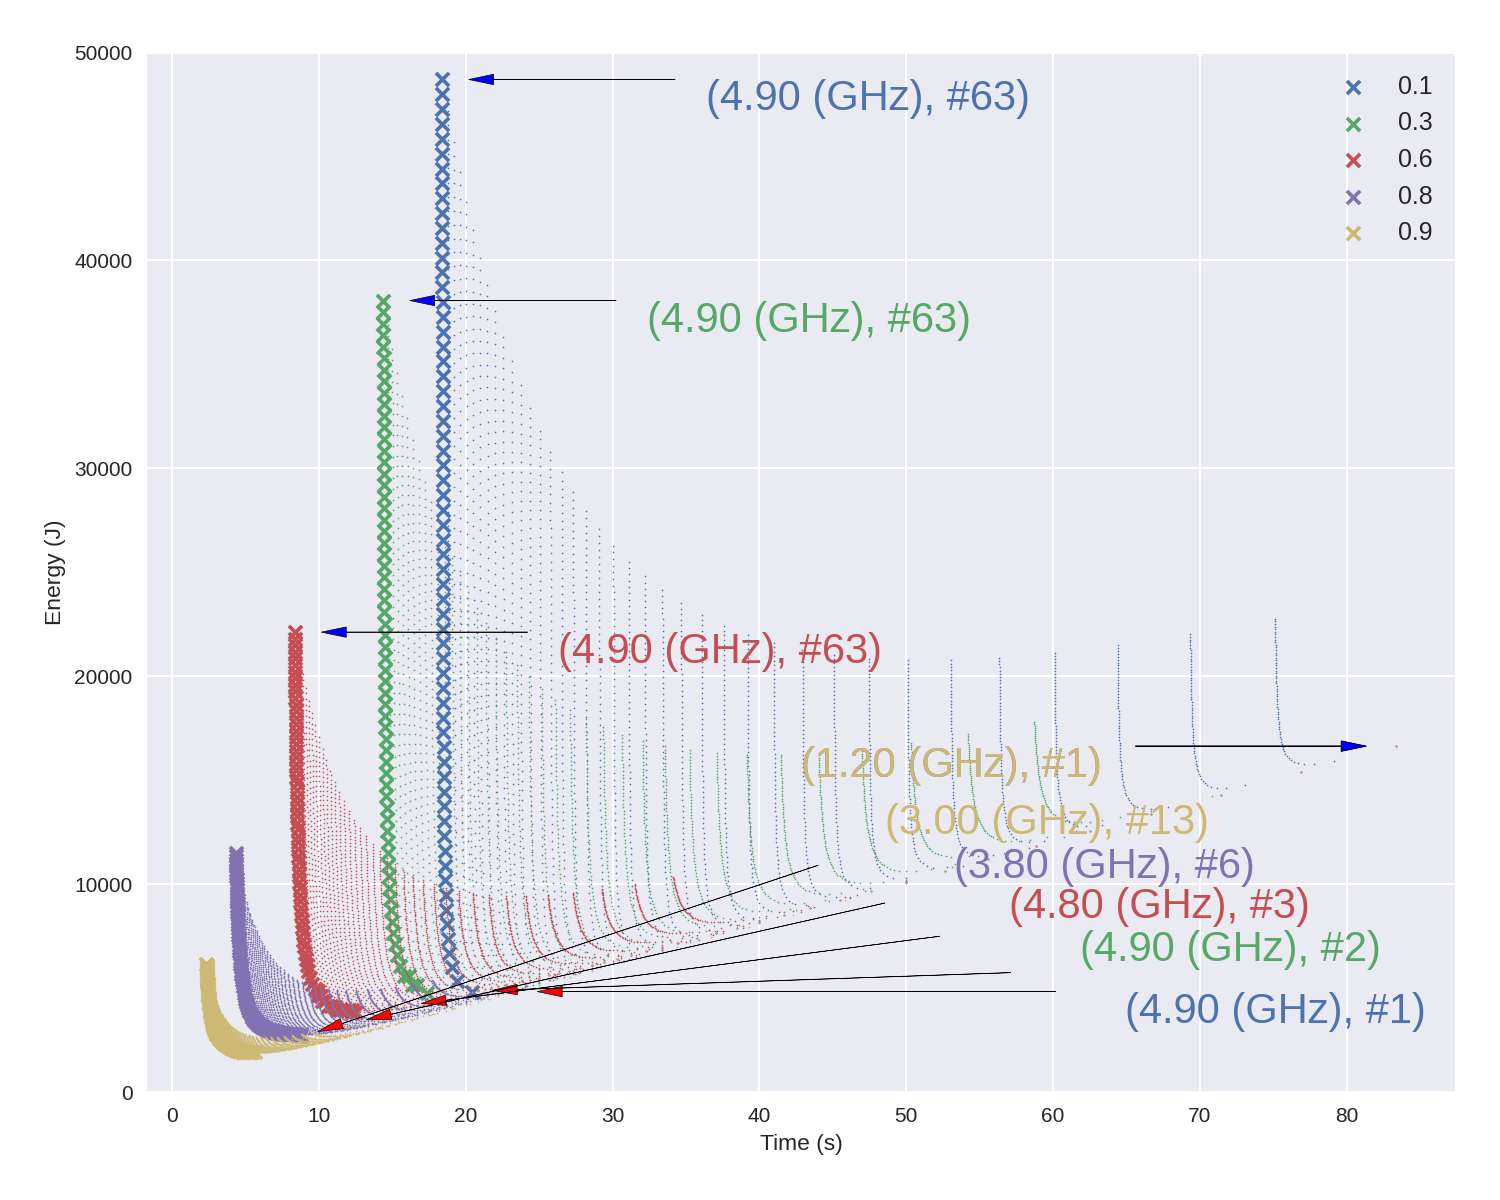
\includegraphics[width=\columnwidth]{models/figures/analisys/pareto_w_high.png}

%	\caption{Pareto w energy}

%	\label{fig:pareto_w_h}

%\end{figure}

%
%\begin{figure}

%	\centering

%	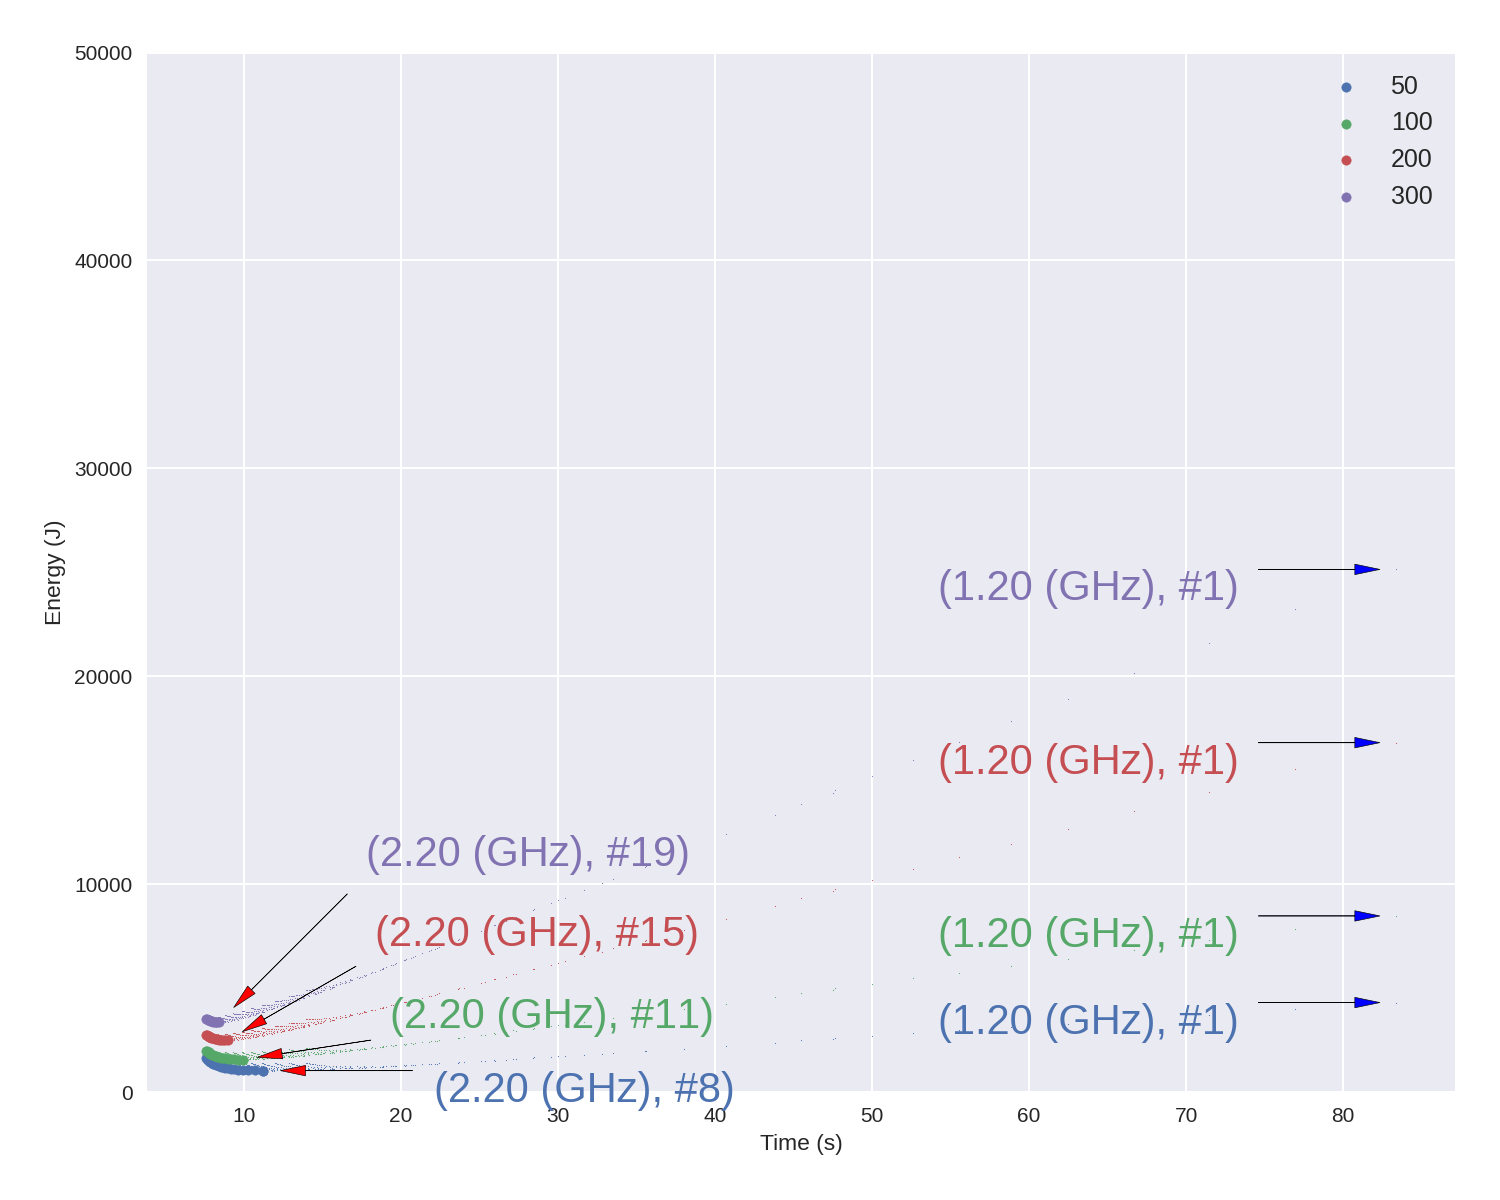
\includegraphics[width=\columnwidth]{models/figures/analisys/pareto_static_low.png}

%	\caption{Pareto w energy}

%	\label{fig:pareto_w_l}

%\end{figure}

%
%\subsection{Optimization under constraints}

%
%\subsection{Gradient and Countorns}

%
%\begin{figure}[H]

%	\centering

%	\begin{subfigure}[b]{0.45\textwidth}

%		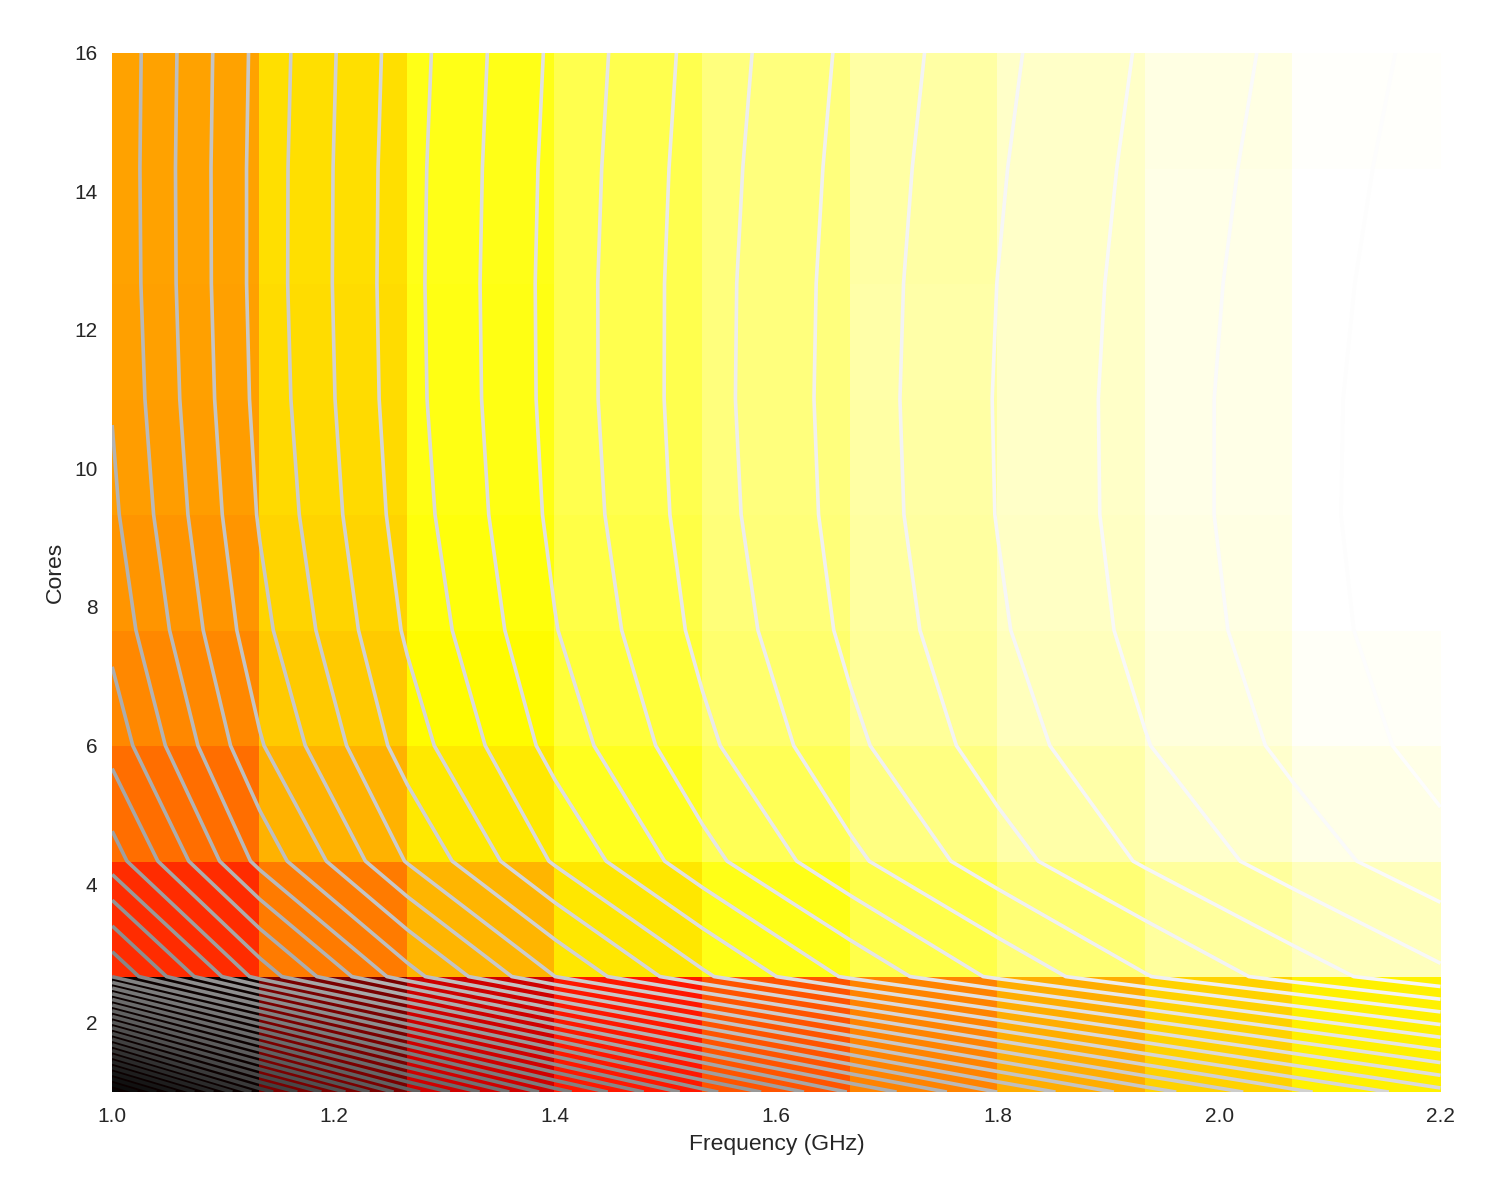
\includegraphics[width=\textwidth]{models/figures/analisys/pdyn0.png}

%	\end{subfigure}

%	%

%	\begin{subfigure}[b]{0.45\textwidth}

%		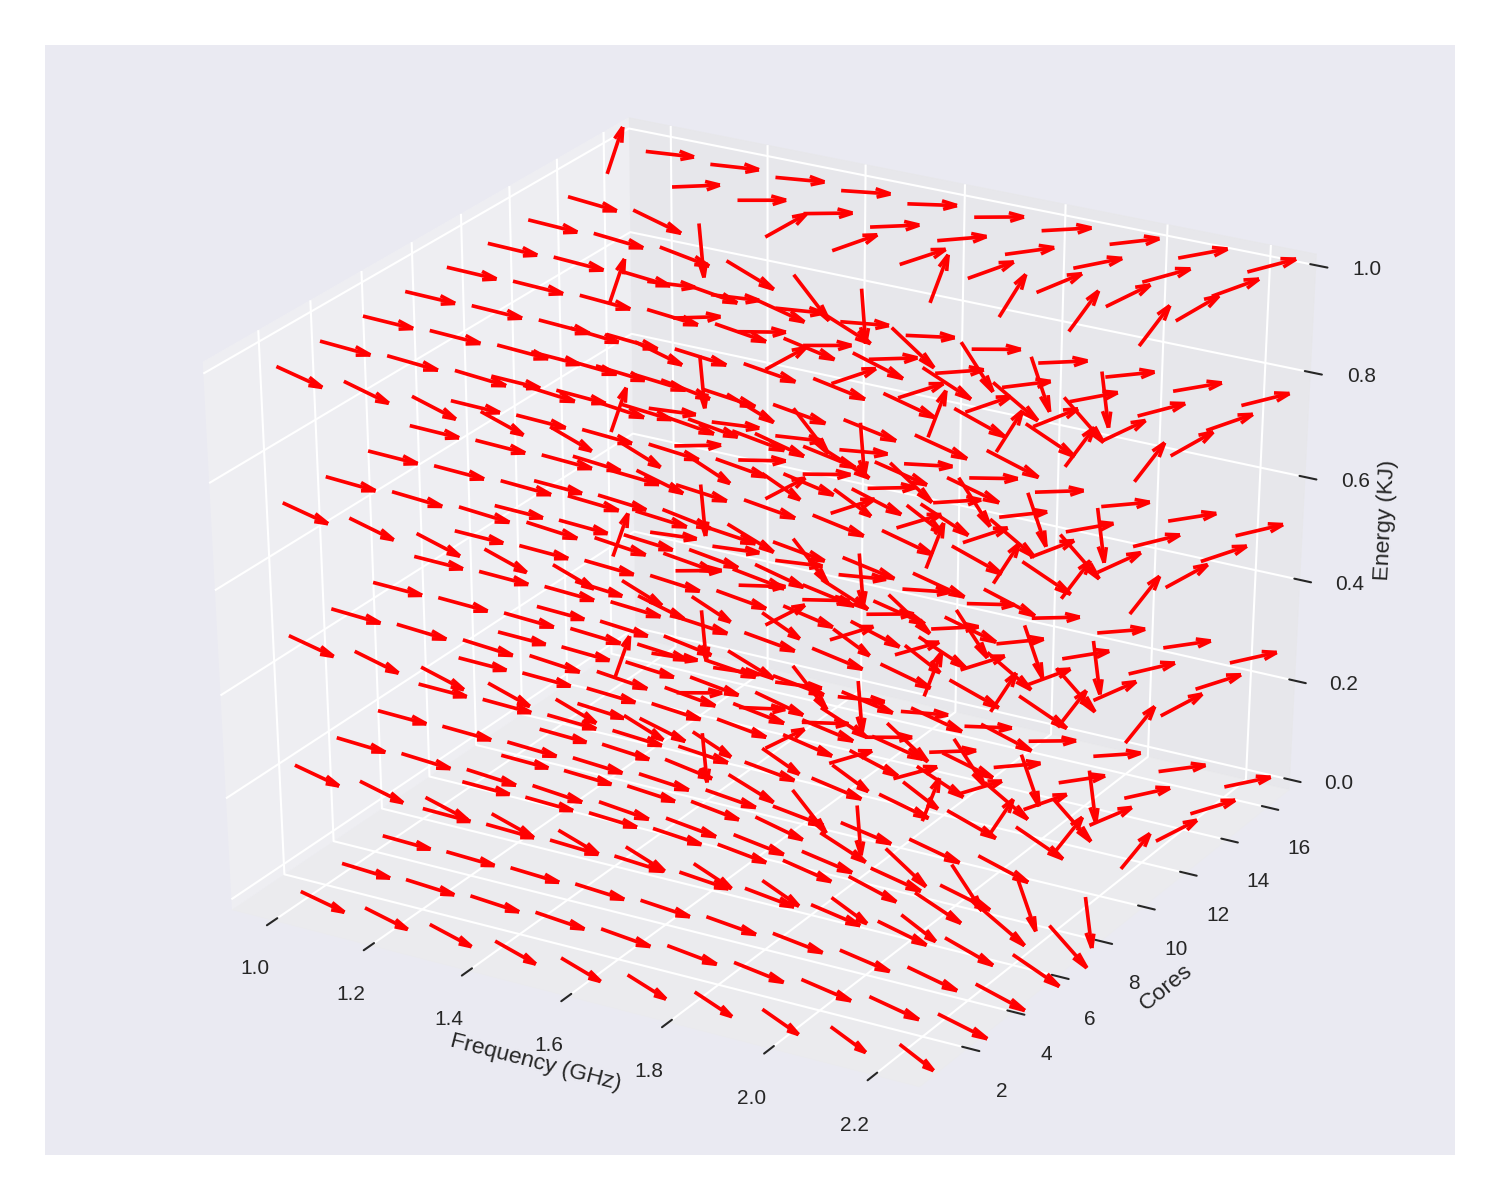
\includegraphics[width=\textwidth]{models/figures/analisys/pdyn0_3d.png}

%	\end{subfigure}

%\end{figure}

%
%\begin{figure}[H]

%	\centering

%	\begin{subfigure}[b]{0.45\textwidth}

%		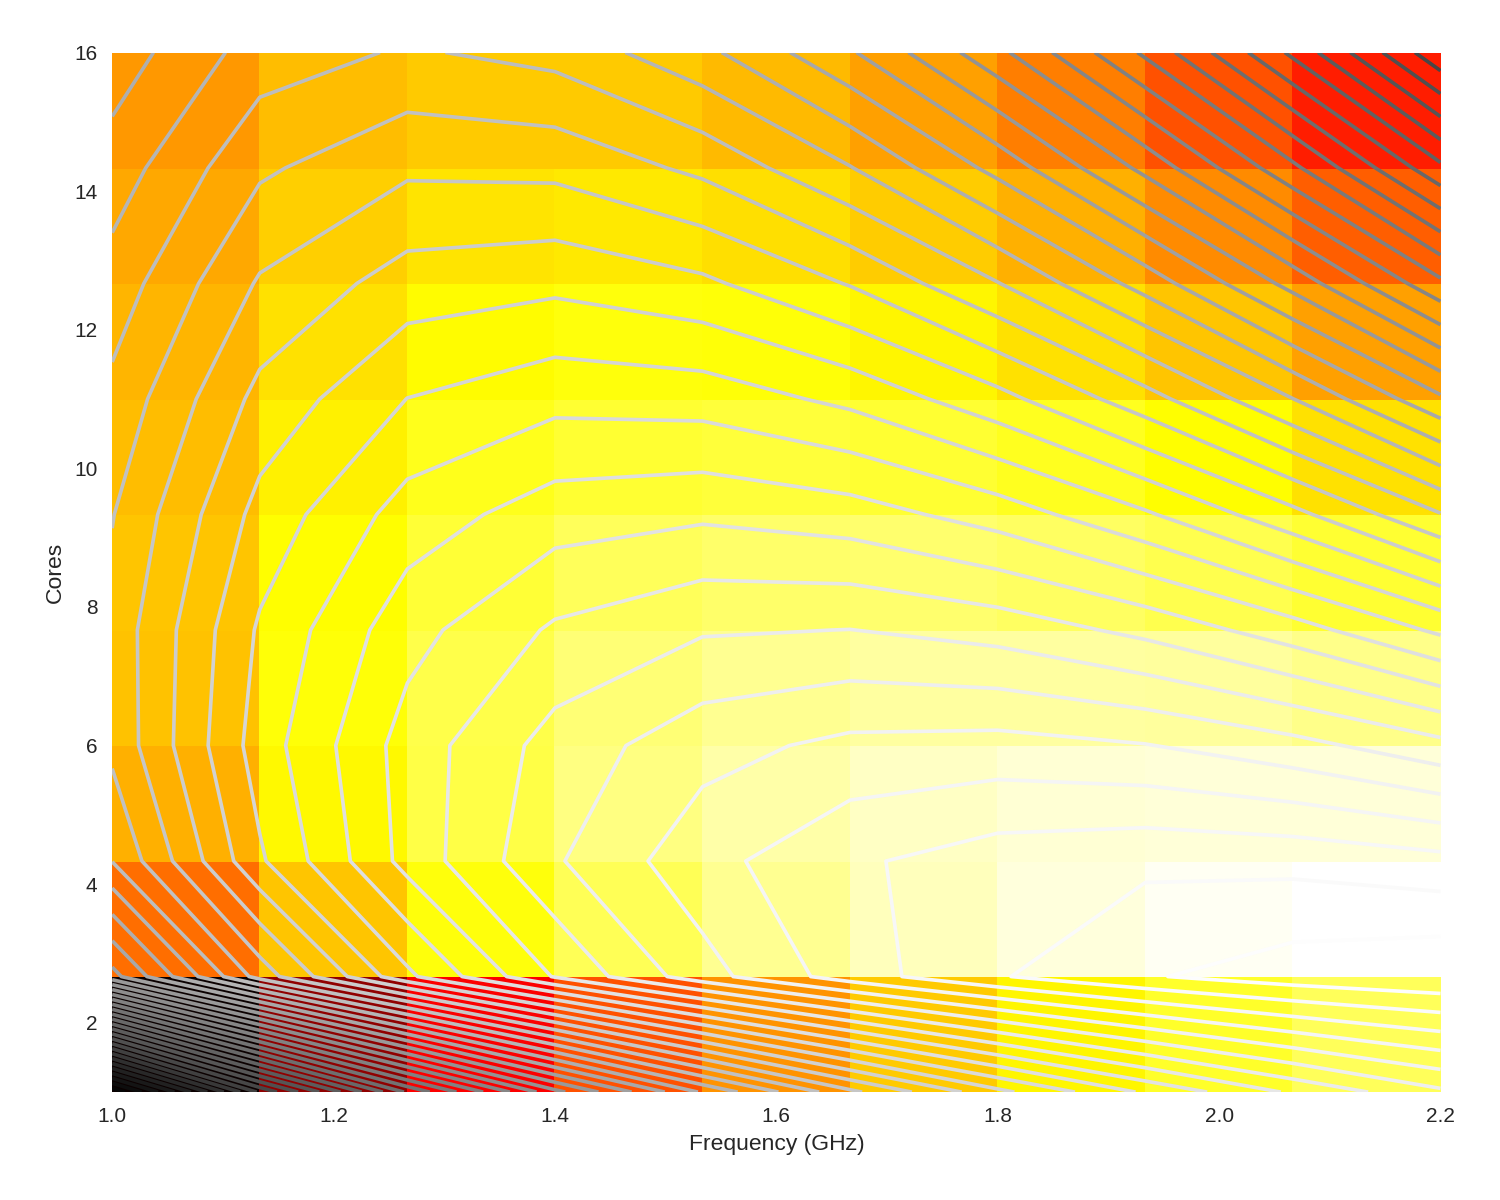
\includegraphics[width=\textwidth]{models/figures/analisys/pdyn3.png}

%	\end{subfigure}

%	%

%	\begin{subfigure}[b]{0.45\textwidth}

%		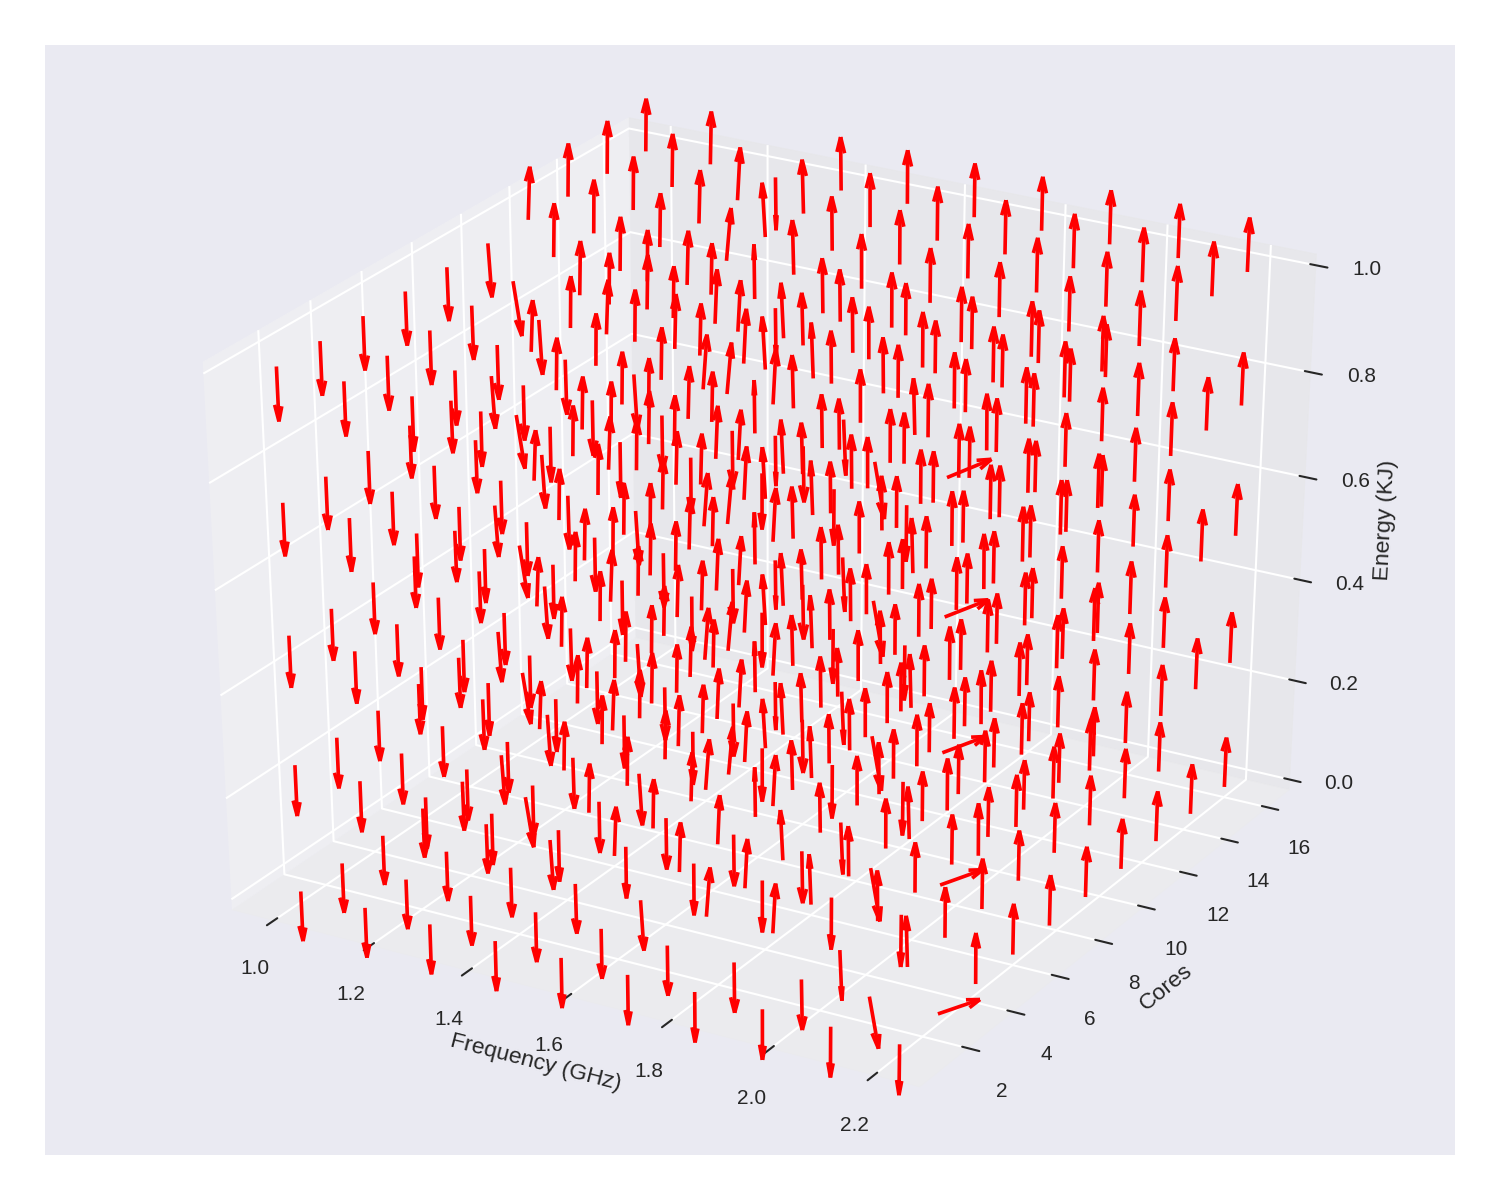
\includegraphics[width=\textwidth]{models/figures/analisys/pdyn3_3d.png}

%	\end{subfigure}

%\end{figure}

%
%\begin{figure}[H]

%	\centering

%	\begin{subfigure}[b]{0.45\textwidth}

%		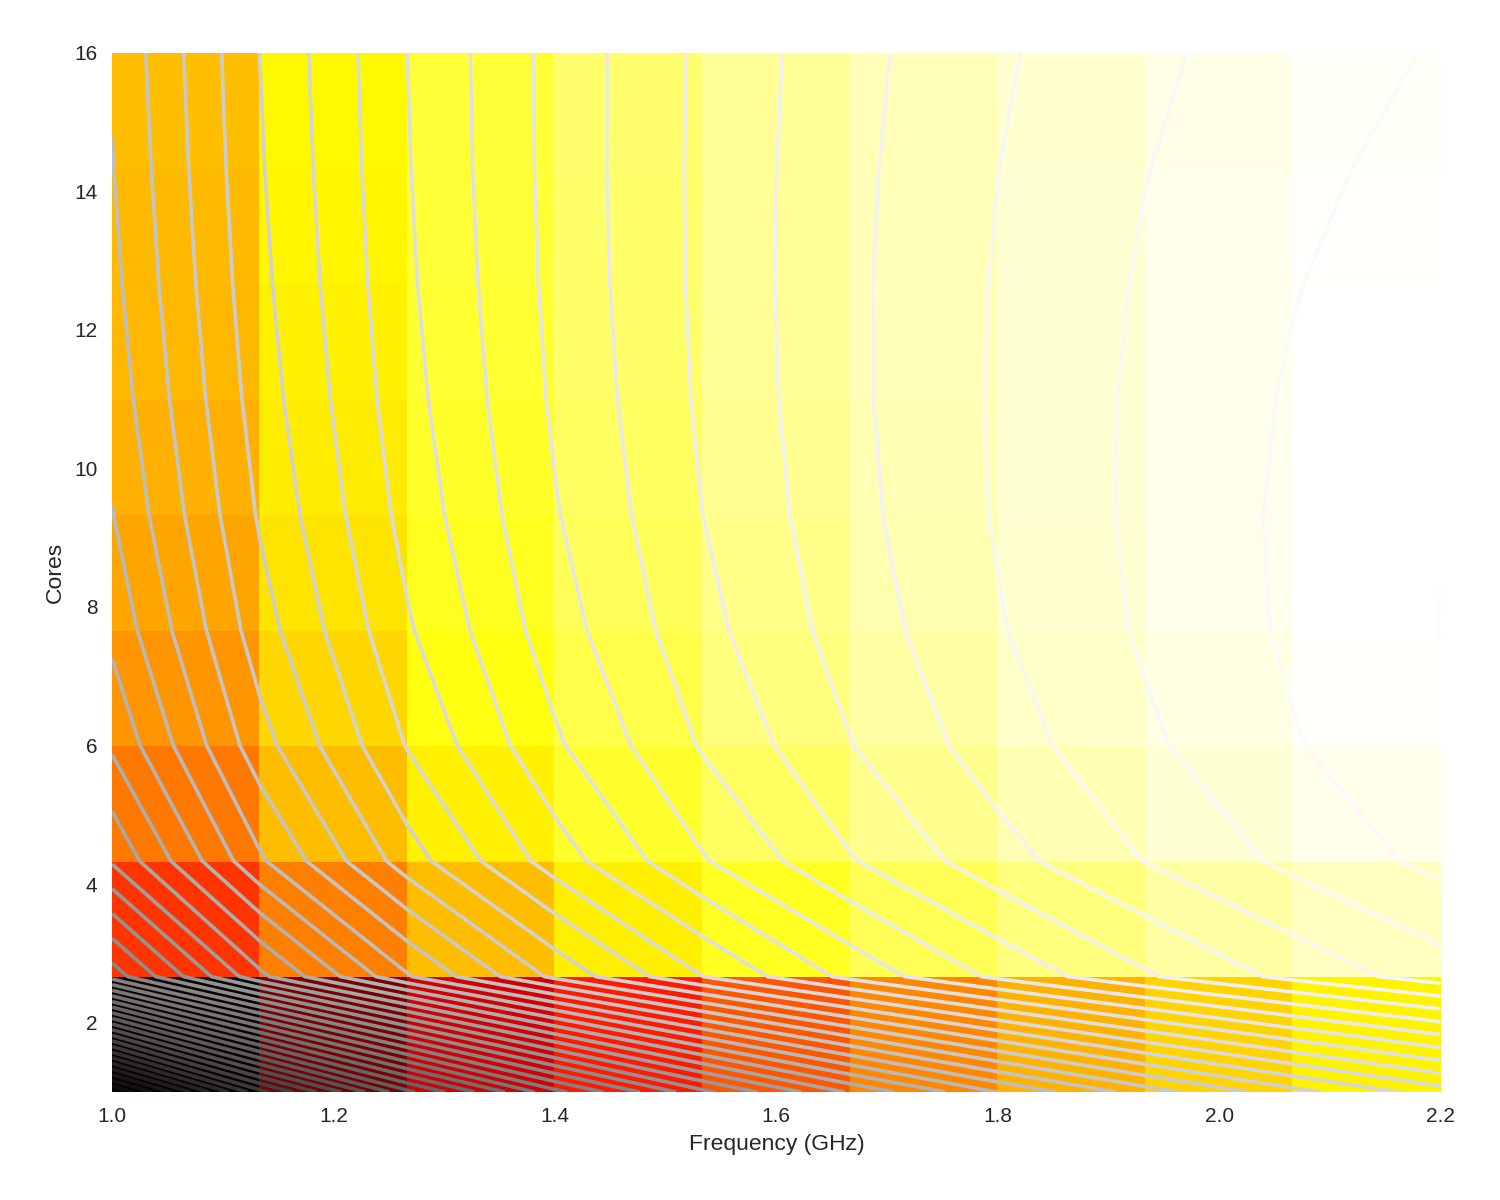
\includegraphics[width=\textwidth]{models/figures/analisys/pleak0.png}

%	\end{subfigure}

%	%

%	\begin{subfigure}[b]{0.45\textwidth}

%		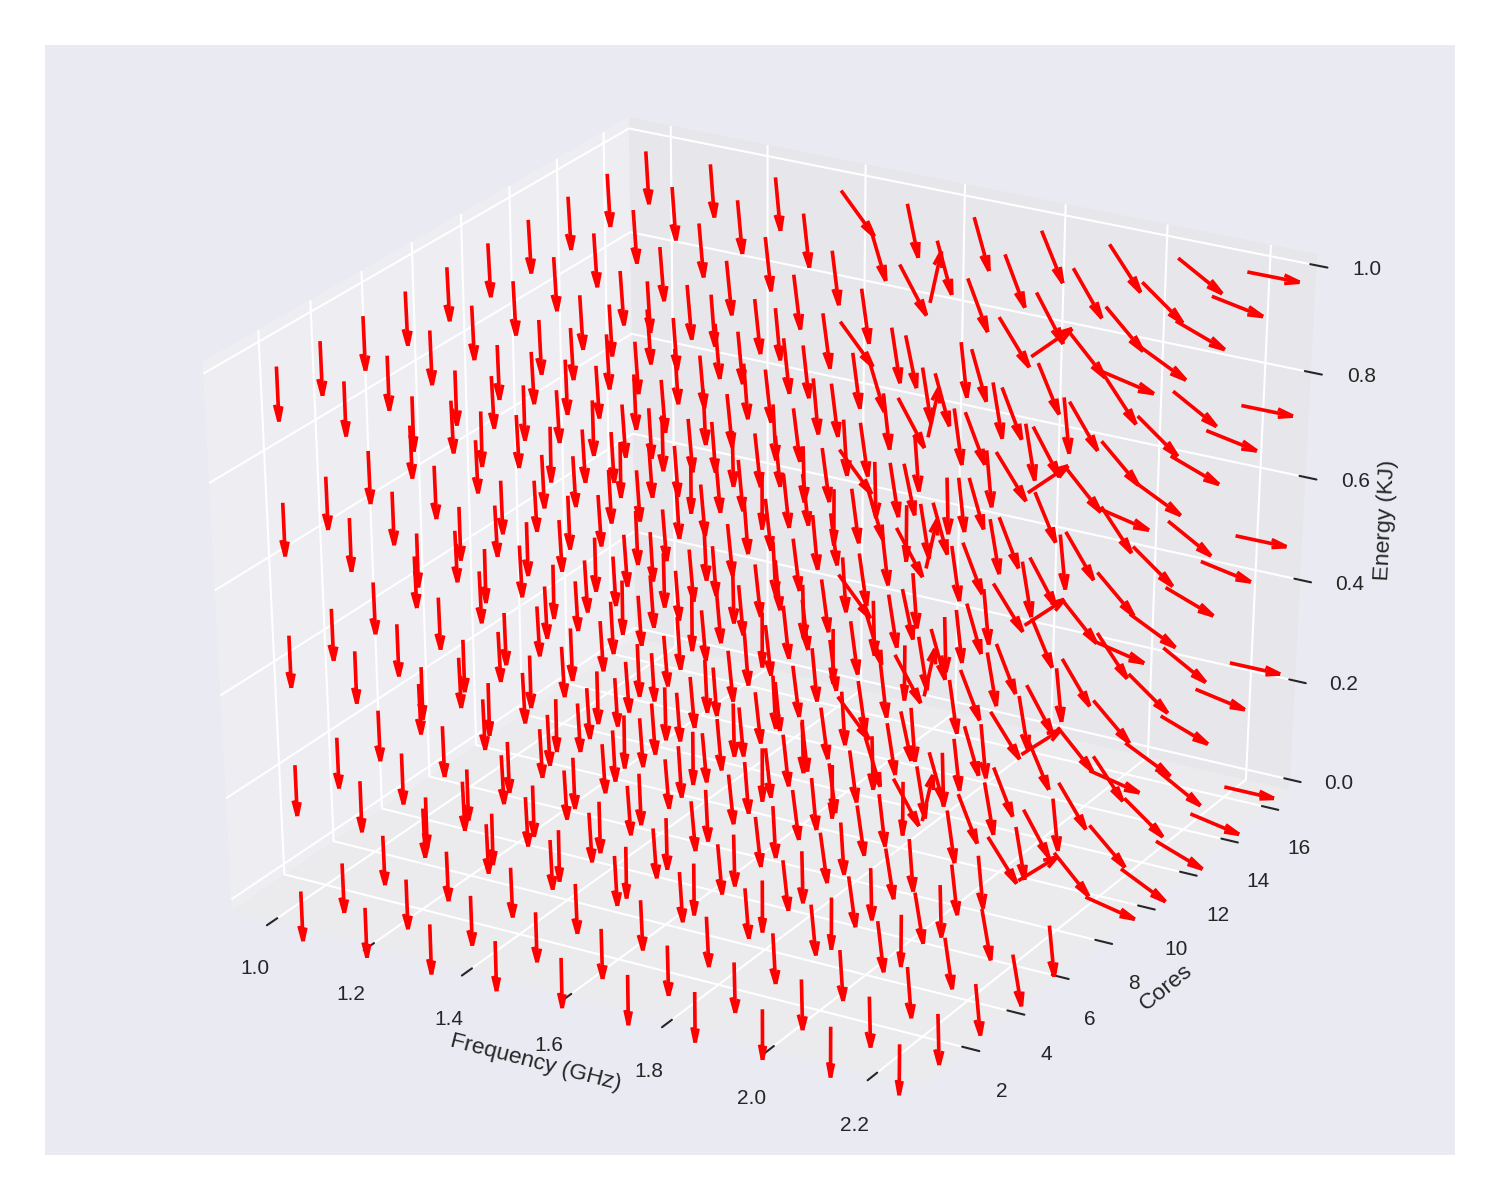
\includegraphics[width=\textwidth]{models/figures/analisys/pleak0_3d.png}

%	\end{subfigure}

%\end{figure}

%
%\begin{figure}[H]

%	\centering

%	\begin{subfigure}[b]{0.45\textwidth}

%		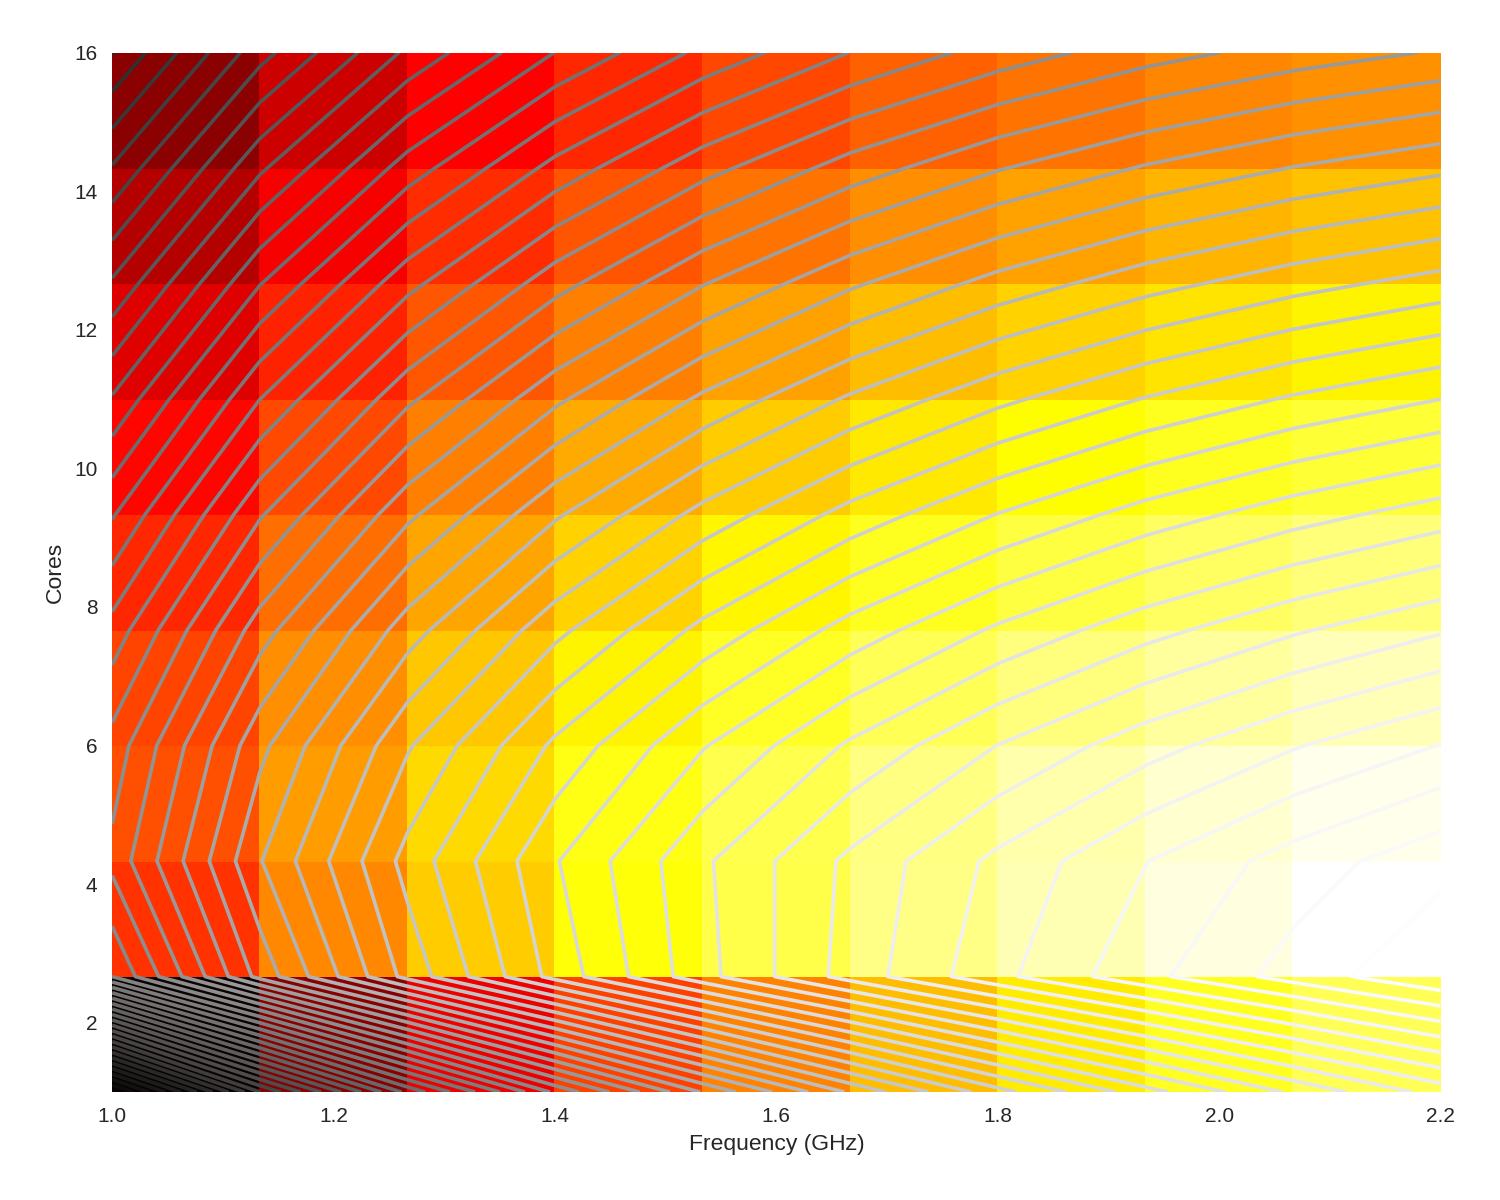
\includegraphics[width=\textwidth]{models/figures/analisys/pleak10.png}

%	\end{subfigure}

%	%

%	\begin{subfigure}[b]{0.45\textwidth}

%		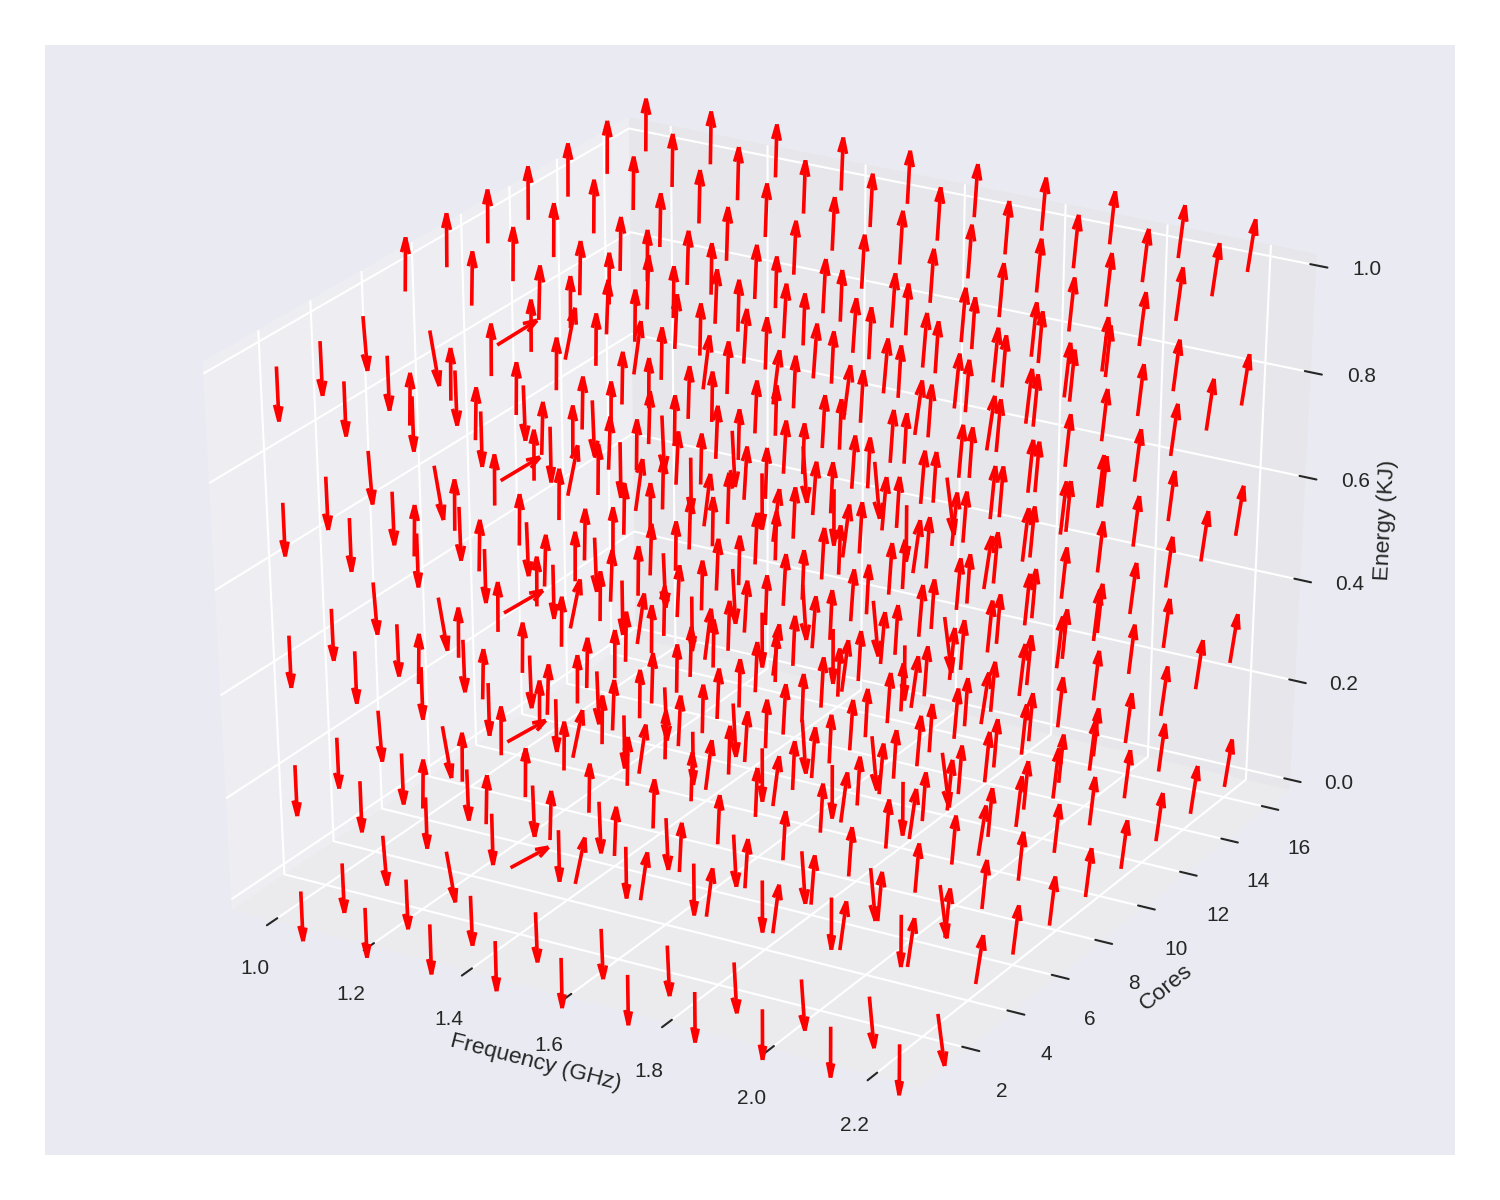
\includegraphics[width=\textwidth]{models/figures/analisys/pleak10_3d.png}

%	\end{subfigure}

%\end{figure}

%
%\begin{figure}[H]

%	\centering

%	\begin{subfigure}[b]{0.45\textwidth}

%		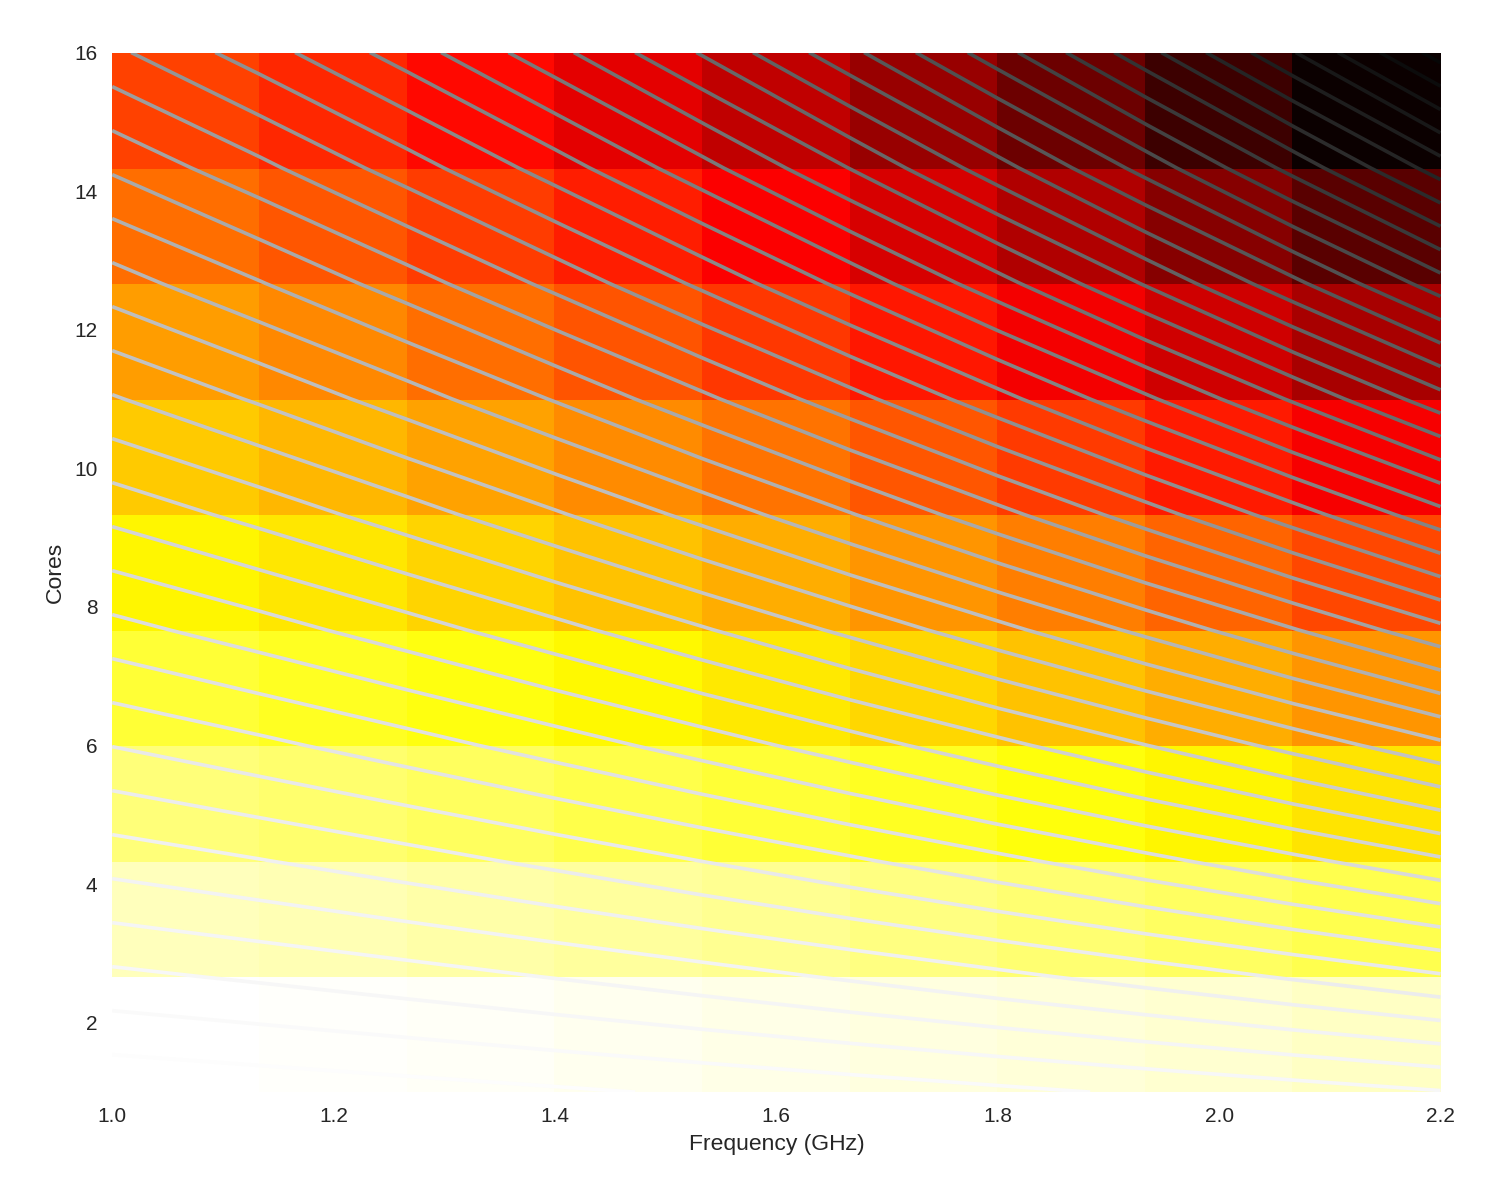
\includegraphics[width=\textwidth]{models/figures/analisys/pstatic0.png}

%	\end{subfigure}

%	%

%	\begin{subfigure}[b]{0.45\textwidth}

%		\includegraphics[width=\textwidth]{models/figures/analisys/pstatic0_3d.png}

%	\end{subfigure}

%\end{figure}

%
%\begin{figure}[H]

%	\centering

%	\begin{subfigure}[b]{0.45\textwidth}

%		\includegraphics[width=\textwidth]{models/figures/analisys/pstatic3000.png}

%	\end{subfigure}

%	%

%	\begin{subfigure}[b]{0.45\textwidth}

%		\includegraphics[width=\textwidth]{models/figures/analisys/pstatic3000_3d.png}

%	\end{subfigure}

%\end{figure}

%
%\begin{figure}[H]

%	\centering

%	\begin{subfigure}[b]{0.45\textwidth}

%		\includegraphics[width=\textwidth]{models/figures/analisys/w0.png}

%	\end{subfigure}

%	%

%	\begin{subfigure}[b]{0.45\textwidth}

%		\includegraphics[width=\textwidth]{models/figures/analisys/w0_3d.png}

%	\end{subfigure}

%\end{figure}

%
%\begin{figure}[H]

%	\centering

%	\begin{subfigure}[b]{0.45\textwidth}

%		\includegraphics[width=\textwidth]{models/figures/analisys/w1.png}

%	\end{subfigure}

%	%

%	\begin{subfigure}[b]{0.45\textwidth}

%		\includegraphics[width=\textwidth]{models/figures/analisys/w1_3d.png}

%	\end{subfigure}

%\end{figure}

